\documentclass[a4paper,10pt]{report}
%
%--------------------   start of the 'preamble'
%
\usepackage{fullpage}
\usepackage{cite}
\usepackage[pdftex]{graphicx}
\usepackage[cmex10]{amsmath}
\usepackage{amstext}
\usepackage[tight,footnotesize]{subfigure}
\usepackage{fixltx2e}
\usepackage{url}
\usepackage{multirow}
\usepackage{latexsym}
\usepackage{amsfonts}
\usepackage{amssymb}
\usepackage{wasysym}
\usepackage{fancyhdr}
\usepackage{array}
\usepackage{longtable}
\usepackage{threeparttable}
\usepackage{acronym}
\usepackage{rotating}
\usepackage{rotate}
\usepackage{eurosym}
\usepackage[utf8]{inputenc}
\usepackage{color}
\usepackage{booktabs}
\usepackage{allrunes}
\usepackage{tabularx}
\usepackage{supertabular}
\usepackage{xcolor}
\usepackage{listings}
\usepackage{fancyvrb,relsize}
\usepackage{caption}
\usepackage{framed}
\usepackage{blindtext}
\usepackage{float}
\usepackage{cprotect}
% always on last place
\usepackage{hyperref}

% hyperref options
\hypersetup{
    colorlinks,%
    citecolor=black,%
    filecolor=black,%
    linkcolor=black,%
    urlcolor=blue % yep, urls are blue and always will be...
}

% special environment for highlights, special concepts, etc.

% hyphenation style
\hyphenation{op-tical net-works semi-conduc-tor}

% new command for short vertical space
\newcommand{\vertbreak}{\vspace{1.75 mm}}

% set caption font size to footnote size
\captionsetup{font={footnotesize}}

%
%%    homebrew commands -- to save typing
\newcommand\etc{\textsl{etc}}
\newcommand\eg{\textsl{eg.}\ }
\newcommand\etal{\textsl{et al.}}
\newcommand\Quote[1]{\lq\textsl{#1}\rq}
\newcommand\fr[2]{{\textstyle\frac{#1}{#2}}}
\newcommand\miktex{\textsl{MikTeX}}
\newcommand\comp{\textsl{The Companion}}
\newcommand\nss{\textsl{Not so Short}}


%
%---------------------   end of the 'preamble'
%
\begin{document}
%-----------------------------------------------------------
\title{\textbf{Understanding Content Dissemination using Content Centric 
Networking} \\ {\large Distributed Systems and Networking Project Report}}
\author{António Rodrigues (up200400437@fe.up.pt)}
\maketitle
%-----------------------------------------------------------
%\begin{abstract}\centering
%A couple of sentences on three or four lines to summarise your work.\\ 
%This is a \LaTeX\ template for undergraduate project reports.\\
%Its detailed contents evolve to reflect FAQs.
%\end{abstract}
%-----------------------------------------------------------
\tableofcontents
%-----------------------------------------------------------
\chapter{Introduction}
\label{chap:intro}

Information-Centric Networking (ICN) is a field of research which advocates for 
a new communication paradigm for the Internet: the departure from 
its host-centric model and the adoption of a content-centric model, enabling 
the direct addressing of content, independently of its 
location. This position is motivated by increasing primary use of the Internet 
for content dissemination, rather than for explicit communication between 
hosts~\cite{Xylomenos2013}.\vertbreak 

This work was prepared as an `hands-on' introduction to 
the field of ICN by taking advantage of the software packages offered by 
Project CCNx~\cite{website:ccnx}, an implementation of the Content Centric 
Networking (CCN) architecture~\cite{Jacobson2009}. We 
run a series of experiments using a simple and exemplifying testbed, evaluating 
the performance of the CCNx implementation over several network parameters and 
its suitability for use in constrained devices.

\section{Content Centric Networking}
\label{sec:intro-ccnx}

Content-Centric Networking (CCN)~\cite{Jacobson2009} presents itself as a 
novel networking paradigm which moves away from the host-centric communication 
model: instead of retrieving content by first determining its location, CCN 
proposes accessing content directly, independently of its location in the 
network, by using content names as addresses.\vertbreak

Communication in CCNs is similar to a publish\slash subscribe model, in the 
sense that it is also driven by 
the consumers of data --- the subscribers --- which release Interest packets 
into the network, eventually received by other CCN nodes. These packets 
announce a subscriber's desire to fetch particular content via the specification 
of a content name field. Holders of content which matches the content name 
--- the publishers --- respond with Data packets, also referred to as Content 
Objects.

\section{Objectives}

The main objectives of this work are the following:\vertbreak

\textbf{1)} Acquire detailed knowledge about a particular ICN approach, by 
            planning and deploying a simple ICN testbed based on 
            Project CCNx~\cite{website:ccnx}, an implementation of the Content 
            Centric Networking (CCN) approach~\cite{Jacobson2009}.\vertbreak

\textbf{2)} Validate some of the benefits claimed by ICN approaches and in some 
            cases compare the network performance of CCNx against equivalent 
            `host centric' solutions. The 
            measurement parameters may vary with each test. Since the 
            objective of CCNs is to reduce latency experienced by clients and 
            network traffic load towards the origins of 
            content~\cite{Jacobson2009}, most of the evaluations are made by 
            comparing values of throughput, latency and network traffic 
            load.\vertbreak

\textbf{3)} We have the clear intention to test the performance of CCNx on 
            `real-world' constrained devices, differing our work from other 
            studies (of different nature), performed in the near-past by Vahlenkamp et 
            al.~\cite{Wahlisch2012, Vahlenkamp2012}. The idea is to evaluate 
            how suitable is the CCNx implementation for direct application 
            in constrained devices such those applied to e.g. Wireless Sensor 
            Networks (WSNs) or Vehicular Networks (VANETS)~\cite{Amadeo2013,Grassi2013}.


\chapter{Content Centric Networking}
\label{chap:ccn}

We now briefly introduce relevant aspects about the Content Centric Networking 
(CCN) paradigm, introduced in Section~\ref{sec:intro-ccnx}.

\section{CCN Packet Types and Content Names}
\label{sec:ccn-packets}

CCN uses two fundamental types of packets: Interest and Data packets (also 
referred to as Content Objects in the scope of Project CCNx~\cite{website:ccnx}, 
a software implementation of the CCN architecture).\vertbreak

\begin{figure}[h!]

    \centering
    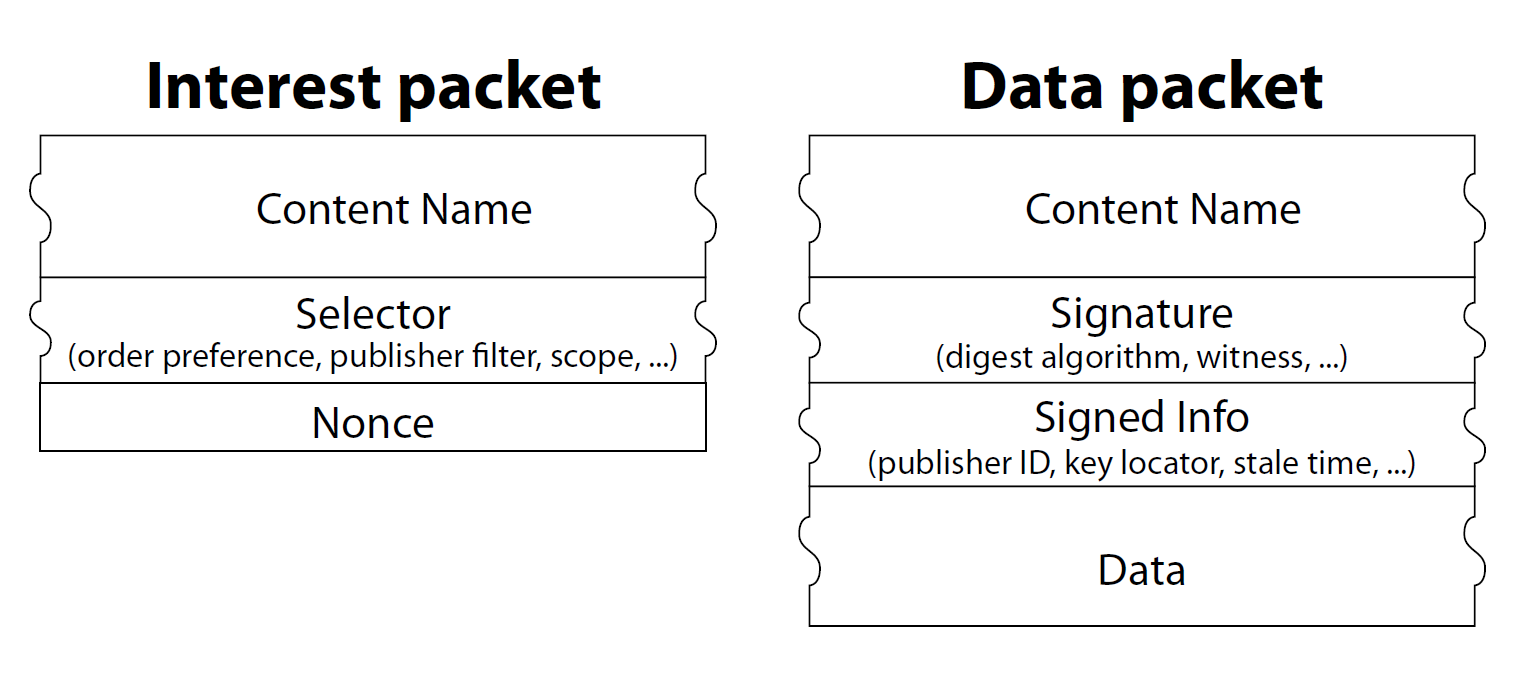
\includegraphics[width=0.65\textwidth]{figures/ccn-packets.png}
    \cprotect\caption{Overview of a CCN Interest and Data packet 
        types~\cite{Jacobson2009}.}
    \label{fig:ccnx-packets}

\end{figure}

Interest packets are originally released into the network by end nodes willing to access a 
particular content, addressing it via its content name. The original paper by 
Jacobson et al.~\cite{Jacobson2009} specifies the use of hierarchical content names, 
e.g. \verb+/sports/football/march.schedule+ (these are also used in practice 
in implementations of CCN, see Section~\ref{subsec:ccnx-specifics}), in order 
to allow publishers to release related content using a single 
prefix and make prefix matching actions intuitive. An Interest packet may 
comprise other fields (e.g. specifying time-limits, maximum number of CCN 
forwarding hops, etc.) and a `nonce' field in order to discard Interest packets 
that may have been duplicated due to network loops (see 
Section~\ref{sec:ccn-forwarding} about CCN forwarding).\vertbreak

Data packets include the content itself with the addition of a cryptographic 
signature. The latter is created by using the data as well as a set of other 
fields such as a timestamp, the publisher's public key (required by other 
nodes to verify signatures), enabling the use of self-certifying names~\cite{Jacobson2009} 
Nodes are supposed to check the signatures and discard any content that fails 
verification.

\section{Forwarding in Content Centric Networks}
\label{sec:ccn-forwarding}

We now introduce the basic forwarding mechanics of a CCN node, starting with 
a description of its inner components.\vertbreak

A CCN node is composed by three main elements: (1) a Forward Information 
Base, (2) a Pending Interest Table (PIT) and (3) a Content Store (CS)~\cite{Jacobson2009}:

\begin{itemize}

    \item \textbf{Forward Information Base (FIB):} Table holding entries 
        which relate a name prefix and a list of interfaces to which 
        Interest packets matching that content name prefix should be forwarded 
        to.
    \item \textbf{Pending Interest Table (PIT):} A table for keeping track of 
        the mapping between arriving Interest packets and 
        the interfaces these have been received from, in order to save a reverse 
        path for Data packets 
        towards one or more subscribers (this may be a 1:N mapping, as an 
        Interest packet matching the same content may be received in 
        multiple interfaces).
    \item \textbf{Content Store (CS):} A cache for content, indexed by Content 
        Name. This is a novel element, allowing for content storage at the 
        Network level. In-network caching allows an Interest to be satisfied 
        by a matching Data packet in any location other than the original 
        producer of the static content, constituting one of the main 
        content-oriented characteristics of CCN.

\end{itemize}

These elements are depicted in Figure~\ref{fig:test-1-1}.\vertbreak

\begin{figure}[h!]

    \centering
    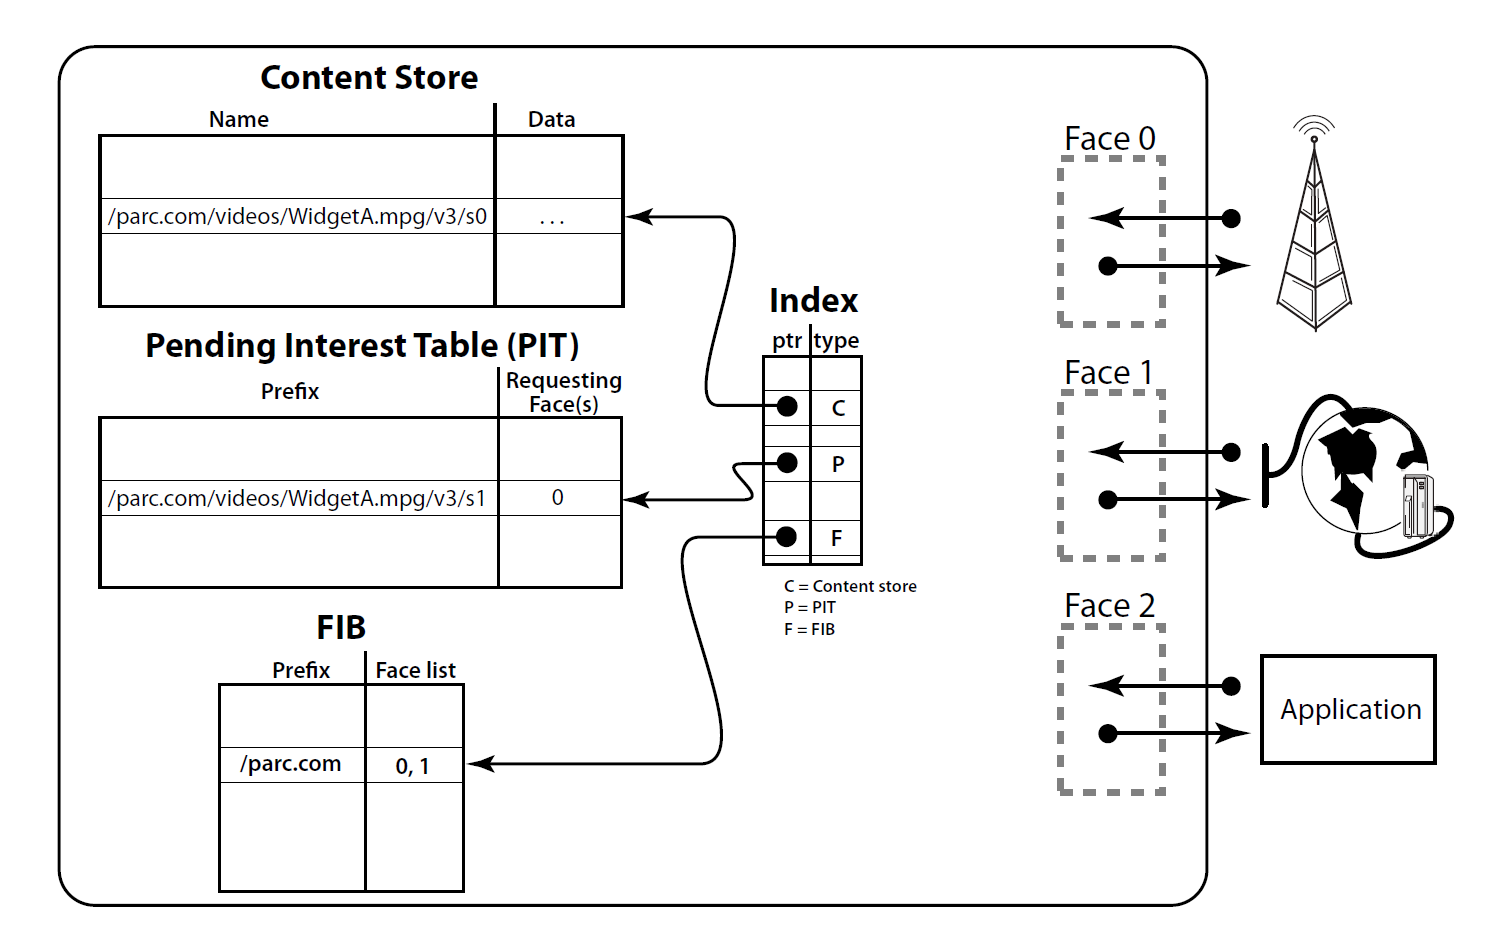
\includegraphics[width=0.65\textwidth]{figures/ccn-node.png}
    \cprotect\caption{Overview of a CCN node's forwarding 
            engine~\cite{Jacobson2009}.}
    \label{fig:test-1-1}

\end{figure}

In CCN, communication is receiver-driven, i.e. having the desire to fetch 
a particular content, an end node releases an Interest packet into the network 
so that it is forwarded towards an appropriate content holder. More precisely, 
an intermediate CCN node performs the following sequence of operations upon the reception of 
an Interest packet~\cite{Jacobson2009}:

\begin{enumerate}

    \item An Interest packet arrives on interface 0 of a given CCN node.
    \item A longest prefix match on the content name specified in the Interest 
        is performed. The CCN node will now look in its CS, PIT and FIB, in 
        that order, in order to resume the forwarding action:
        \begin{enumerate}

            \item If there's a match on the node's CS, a copy of the respective 
                CS entry will be sent back via interface 0, the Interest 
                packet is dropped. \textbf{End.}

            \item Else if there is an (exact) match on the PIT, interface 0 is 
                added to the mapping list on the respective entry. The 
                Interest packet is dropped (as a previous one has already been 
                sent upstream). \textbf{End.}

            \item Else if only a matching FIB entry is found, the Interest 
                packet is forwarded upstream, via all remaining interfaces on the 
                list (other than 0), towards an eventual content holder. A PIT 
                entry $<$content name, interface 0$>$ is added. \textbf{End.}

            \item Else if there is no match at all, the Interest packet is 
                simply discarded. \textbf{End.}

        \end{enumerate}

\end{enumerate}

Note that in CCN 
only Interest packets are routed: as the intermediate CCN nodes forward the 
Interests, their respective PIT tables are updated with Interest-to-interface 
mappings, pre-establishing a reverse path for Data packets to follow as a 
content holder is found. When the reverse path is started by a CCN node 
holding a particular content name, each intermediate CCN node receiving a 
Data packet looks in its PIT for $<$content name, interface n$>$ entries, 
and forwards the Data packet through all matching interfaces. In addition, a 
CS entry is created to cache the content locally at the node. If a Data packet 
with no matching PIT entries arrives, it is treated as unsolicited and discarded.

\chapter{Methodology}

We evaluate the performance of an available ICN 
implementation --- Project CCNx~\cite{website:ccnx}\,\footnote{We henceforth 
address the CCN networking concept as `CCN' and its implementation as `CCNx'.} --- 
by setting up a simple testbed, composed by commercial off-the-shelf (COTS) 
equipment. Besides validating some of the claims made by CCN, we attempt to 
compare CCNx applications to equivalent `host centric' solutions.\vertbreak

This section (1) describes the CCNx software 
package to be used in the tests, (2) provides an overview of the testbed's 
structure and (3) details the protocol of the tests to be conducted.

\section{Project CCNx}

Project CCNx~\cite{website:ccnx} provides an open source software reference 
implementation PARC's CCN architecture~\cite{Jacobson2009}, with the 
objective of enabling experimentation in the network research community. The 
project provides APIs written in multiple programming languages (C, Java and 
Android), with extensive documentation.\vertbreak

CCNx is designed to run on top of 
existing transport protocols and addressing schemes --- TCP, UDP, 
etc. --- in an `overlay' approach. This means that CCNx packets are tunneled 
within TCP or UDP flows running over IP. Although Project CCNx developers 
present this as a short-term approach for developers to start trying 
CCN, it is also presented as a feature, implying CCN's advantage over similar 
solutions in the current networking paradigms (e.g. web 
caching)~\cite{Jacobson2009,website:ccnx,Willis2012,Melazzi2012}.

\subsection{CCNx Applications}

Project CCNx 
provides the following ensemble of example applications~\cite{Muther2012a}:

\begin{itemize}

    \item \verb?ccnchat?: Simple application for real-time transmission of text 
            messages from sender to receiver.
    \item \verb?ccnfileproxy?: Allows one to share files within the 
            node's file system to other CCNx 
            nodes\textsuperscript{\ref{foot:note1}} (used as an alternative to 
            setting up a CCNx repository~\cite{Muther2012a}).
    \item \verb?ccnputfile?\,\slash\,\verb?ccngetfile?: Pair of applications to 
            write\slash read files to\slash from CCNx nodes, e.g. to store 
            files into a CCNx repository.
    \item \verb?ccnsendchunks?: Simple application 
            which divides a given piece of content in `chunks' upon the 
            reception of Interest packets directed at that same content, and 
            sends the `chunks' as Data packets towards the requester. Interest 
            packets are generated via the complementing \verb?ccncatchunks2?
            application.
    \item VLC CCNx plugin: Plugin to the VLC media player~\cite{website:vlc}, 
            which allowing a CCNx node to remotely playback a video stored on a 
            CCNx repository, identified by its `content name'.
    \item Others (see Section `What To Look At' in~\cite{Muther2012a}).

\end{itemize}

The diversity of application types listed above may translate into a reasonably 
sized set of test possibilities. However, their specific CCNx implementations may 
significantly differ from those one would use in the non-CCNx case (e.g. 
\verb?ccnchat? vs. an established instant messaging application 
or protocol e.g. XMPP). The influence of implementations should be taken 
into account when analyzing network performance results.\vertbreak

\subsection{Specificities of CCNx Applications}
\label{subsec:ccnx-specifics}

Here we provide CCNx application-specific information, useful for understanding the 
tests and results shown in later sections.

\subsubsection{CCNx Forwarding Tables}
\label{subsubsec:fibs}

Since CCNx works as an `overlay', CCN's routing scheme based on content must be 
translated into IP routing at a given point. In CCNx this is accomplished 
by the routing daemon, \verb+ccnd+, the main process running in CCNx 
nodes~\cite{website:ccnx-commands}.\vertbreak

As dynamic routing in CCNs is still an area of current research 
and not well supported by current CCNx releases~\cite{Wang2012,Hoque:2013:NNL:2491224.2491231}, 
we adopt the same strategy as that applied in previous work~\cite{Wahlisch2012, Vahlenkamp2012} 
and manually added static routes to CCNx's Forwarding Table (FIB), using the 
\verb+ccndc+ utility~\cite{website:ccnx-commands}. We provide examples of 
the \verb+ccndc+ command in Appendix~\ref{app:ccnx-specificss}.

\subsubsection{Disseminating Content with CCNx}
\label{subsubsection:disseminating-ccnx}

In CCNx, content sources use a specific repository application for storing 
content and make it available in CCNx networks by responding to 
matching Interests, \verb+ccnr+~\cite{website:ccnx-commands}. The \verb+ccngetfile+ application~\cite{website:ccnx-commands} 
can then be used to release Interest packets to the CCNx network, querying 
for particular content. Appendix~\ref{app:ccnx-specificss} presents some concrete examples 
of the usage of these applications.\vertbreak

CCNx also provides \verb+ccnsendchunks+ and \verb+ccncatchunks2+, another duet 
of applications for content exchange. \verb+ccnsendchunks+ takes content (e.g. 
a file) as input, and produces Data packets containing `chunks' of the content 
(blocks of a given size, in byte) as it receives Interests, or at a rate of 
one-per-second, whichever is faster\,\footnote{Although no 
MAN page exists for this command, the following resource may be used as an unofficial 
source of information: \url{https://www.ccnx.org/pipermail/ccnx-dev/2010-April/000189.html}.}. 
The complementary Interest-producing \verb+ccncatchunks2+ also uses pipelining 
of Interests, varying 
its `window size' according to the rate of arrival of Data packets. This 
behavior is also analyzed in some of the tests specified in 
Section~\ref{sec:protocol}. We provide examples of the use 
of both commands in Appendix~\ref{app:ccnx-specificss}.\vertbreak

Video content stored in a CCNx repository may be directly played back in 
VLC media player~\cite{website:vlc}, using a special CCNx plugin which 
generates Interests for that content (any type of content playable by VLC, 
e.g. a \verb+.avi+ file), receives the respective Data packets, decodes them 
and progressively plays them back. Again, we provide examples of its 
usage in Appendix~\ref{app:ccnx-specificss}.

\section{Testbed Description}
\label{sec:testbed}

The basic testbed structure used for evaluation of CCNx is depicted in 
Figure~\ref{fig:basic-testbed}. Some tests require alterations to this scheme, 
nevertheless such alterations are promptly indicated 
in the individual test descriptions, in Section~\ref{sec:protocol}. Table~\ref{tab:hw} 
provides a list with more details of the testbed equipment.\vertbreak

\begin{figure}[h!]

    \centering
    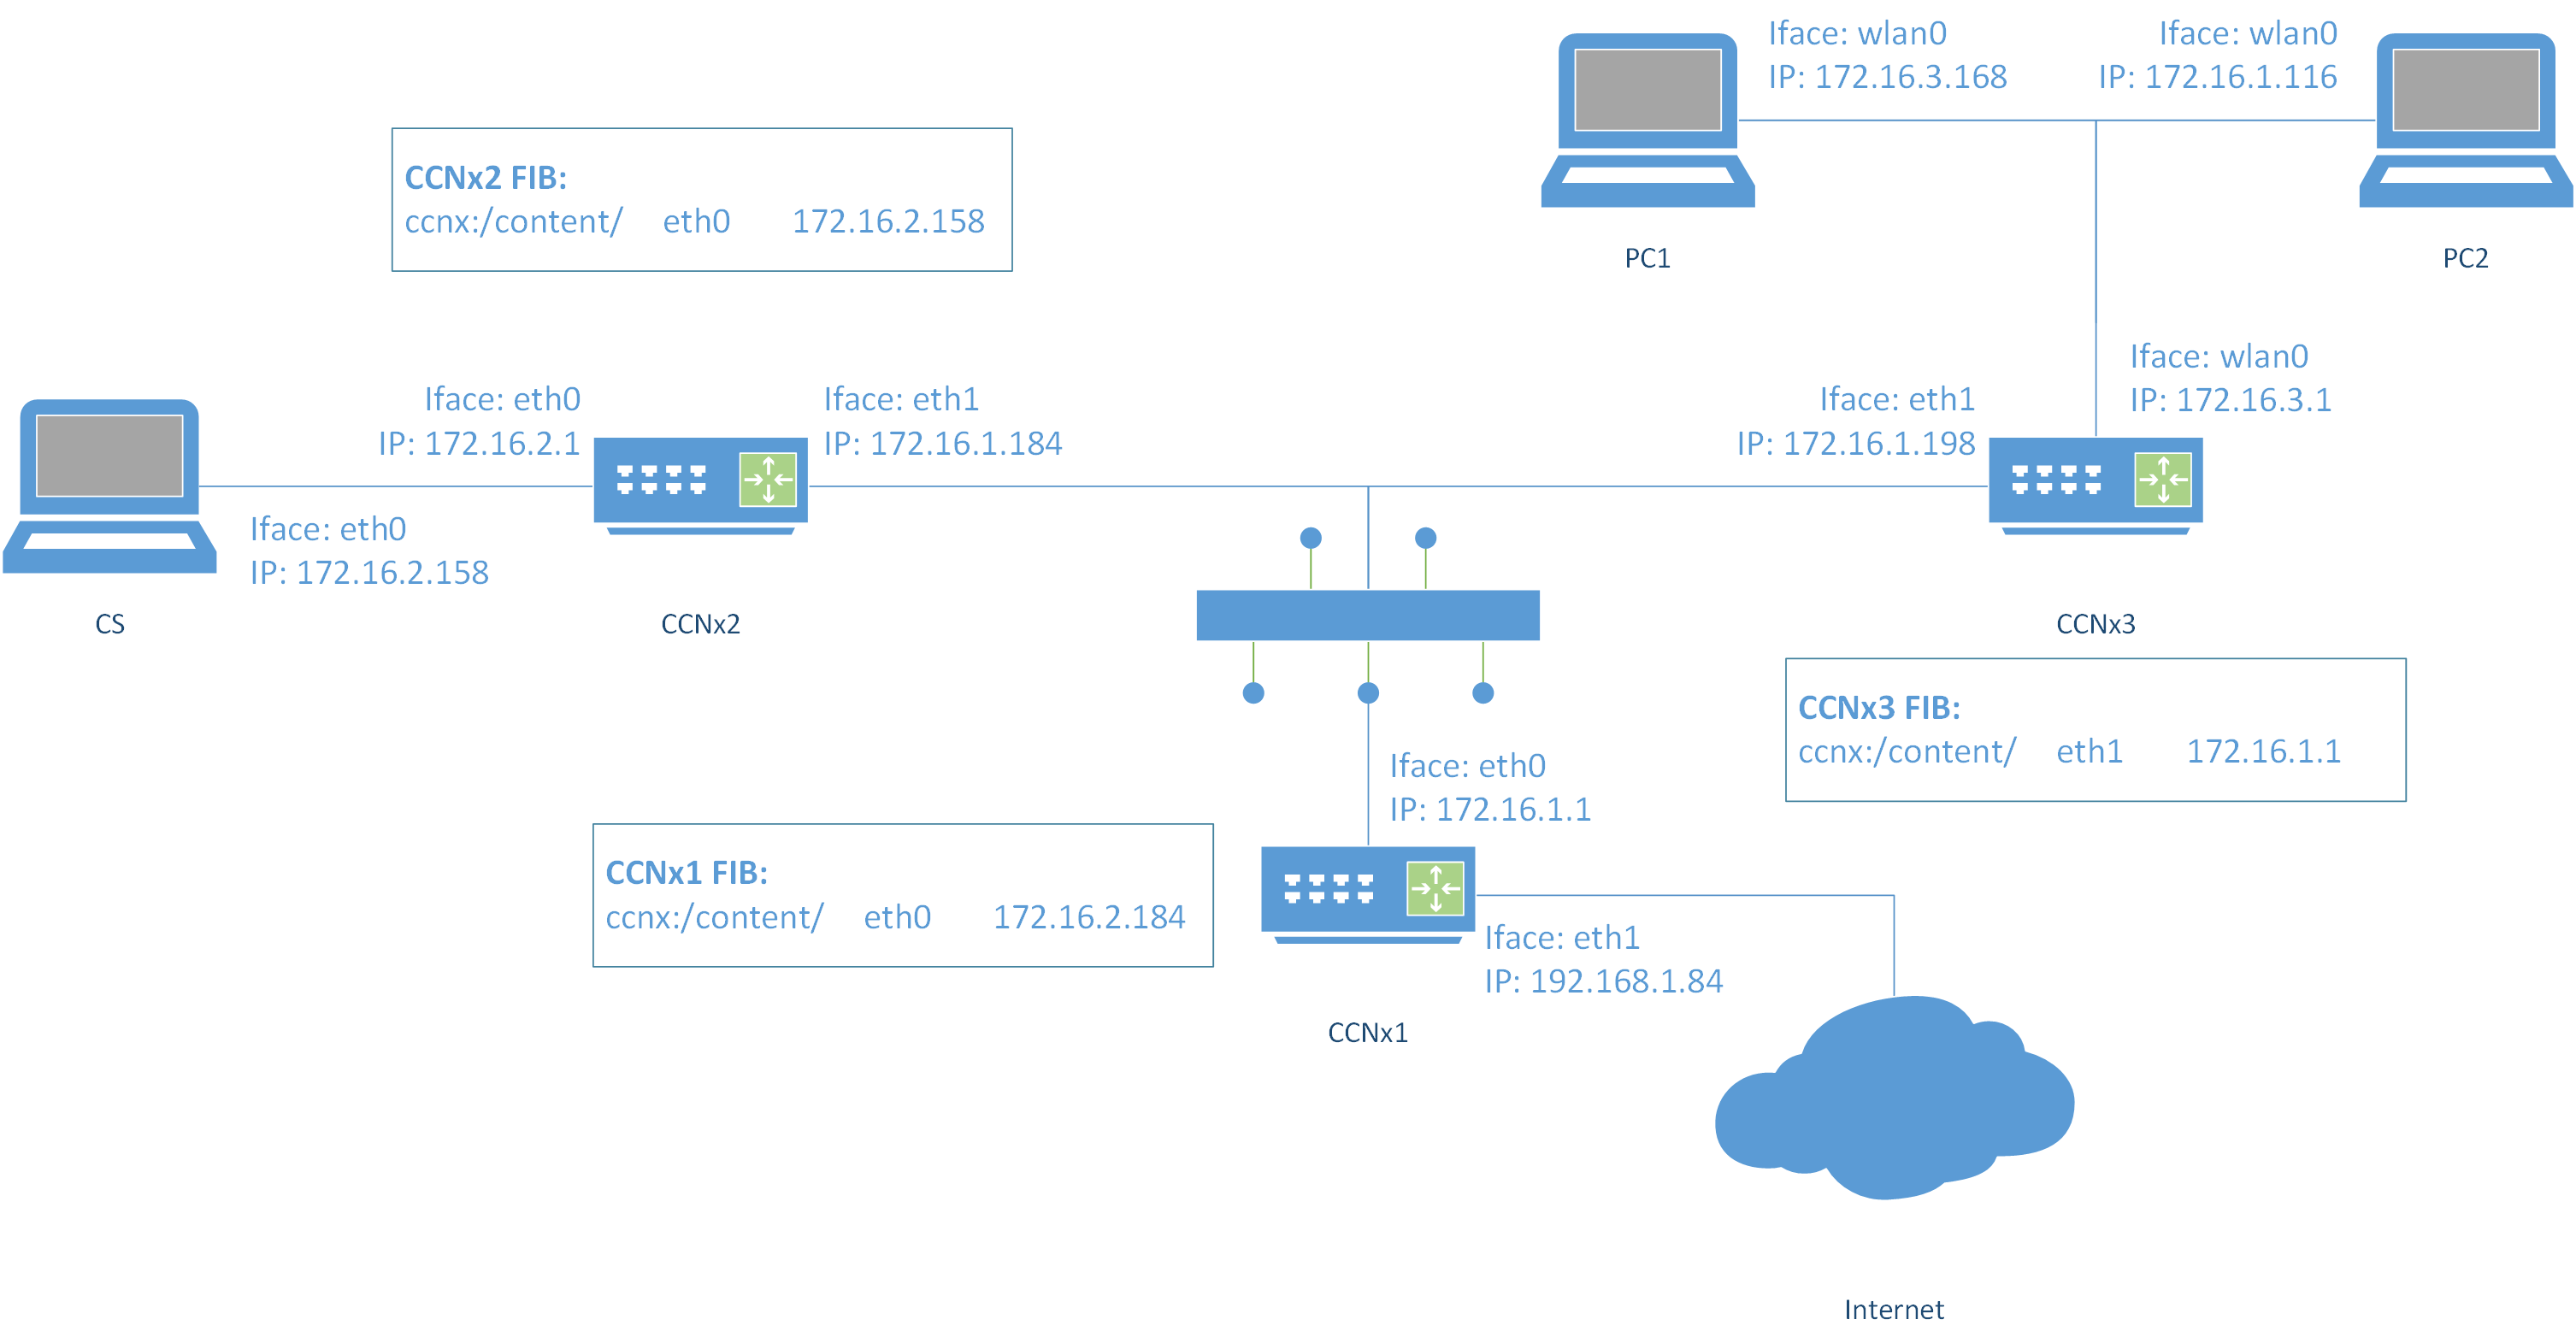
\includegraphics[width=0.80\textwidth]{figures/diag1.png}
    \cprotect\caption{Basic arrangement for the proposed testbed.}
    \label{fig:basic-testbed}

\end{figure}

The basic scenario depicted above includes 3 COTS residential routers, labeled 
as `CCNx1', `CCNx2' and `CCNx3' (Linksys WRT160NL) running OpenWRT\,\footnote{`Barrier 
Breaker' version, SVN revision 35323, available at \url{https://dev.openwrt.org/browser/trunk?rev=35323}.}~\cite{website:openwrt}, a Linux-based 
operating system. These represent the Inner Nodes (INs) of a network, 
serving as CCNx\slash IP routers (see Section~\ref{subsubsec:ccnx-openwrt} for details on the 
installation of CCNx software on embedded Linux systems). Table~\ref{tab:hw} 
summarizes the hardware specifications of these devices.\vertbreak 

The arrangement 
separates the End Nodes (ENs) --- consumers of content --- and the Content 
Sources (CSs) --- generators of content --- in different 
IP subnets (172.16.x.x), so that routing is performed in both CCNx and `host centric' 
scenarios\,\footnote{As CCNx works as an overlay, IP routing will be performed 
in both CCNx and `host centric' test versions. Nevertheless, as this work may 
potentially origin subsequent research (e.g. testing dynamic routing in CCNx), 
we believe it is good practice to test this scenario from the start}.\vertbreak

\begin{table}[h!]
    \centering
    \footnotesize
        \begin{tabularx}{1.00\textwidth}{ l l X X c }
            %\hline
            \toprule
            \textbf{Test Element} & \textbf{Label(s)} & \textbf{Type} & \textbf{Relevant Specs.}  & \textbf{Qty.} \\ [0.5ex]
            \midrule
            \multirow{2}{*}{Content Source(s)} & \multirow{2}{*}{CS} & \multirow{2}{*}{Laptop (w\slash Ubuntu 12.04)} & Wi-Fi: 802.11 b/g & \multirow{2}{*}{1} \\ [0.5ex]
                                               & & & Ethernet: 10\slash 100\,Mbps & \\ [0.5ex]
\midrule
            \multirow{4}{*}{Inner Node(s)}  & CCNx1 & \multirow{4}{*}{Linksys WRT160NL~\cite{website:wrt160nl}} & CPU: Atheros 9130-BC1E 400 Mhz    & \multirow{4}{*}{3} \\ [0.5ex]
                                            & CCNx2 &              	& RAM: 32 MB                        & \\ [0.5ex]
                                            & CCNx3 &               & Wi-Fi: 802.11 b/g/n               & \\ [0.5ex]
                                            & &                     & Ethernet: 10\slash 100\,Mbps      & \\ [0.5ex]
            \midrule
            \multirow{2}{*}{End Node(s)}    & PC1   & \multirow{2}{*}{Laptop (w\slash Ubuntu 12.04)}    & Wi-Fi: 802.11 b/g/n & \multirow{2}{*}{2} \\ [0.5ex]
                                            & PC2   &                                                   & Ethernet: 10\slash 100\,Mbps      & \\ [0.5ex]
            \bottomrule
        \end{tabularx}
    \caption{Table of hardware for the testbed depicted in Figure~\ref{fig:basic-testbed}.}
    \label{tab:hw}
\end{table}

\subsection{Testbed Setup Details}

%This section documents pertinent notes about the testbed setup process, 
%specifically related to the installation of CCNx at the network nodes.

\subsubsection{Setting up CCNx at End Nodes (ENs)}

We have used the latest release of CCNx (0.8.1)\,\footnote{Compiled from source, 
available at \url{http://www.ccnx.org/software-download-information-request/download-releases/}} at the EN nodes. 
In addition to the basic CCNx package, the VLC plugin (available with CCNx 0.8.1 package)
was separately compiled and installed at the ENs, in order test dissemination 
of video content in CCNx networks. The VLC version 2.0.8 TwoFlower was used 
for testing at the ENs.\vertbreak

As the objective of the work is to monitor the performance of CCNx according to 
network parameters such as network load, throughput, latency, etc. a patched 
version of Wireshark (version 1.8.6) was re-compiled to include a CCN packet 
dissector~\cite{website:ccn-wireshark}.

\subsubsection{Setting up CCNx at Inner Nodes (INs)}
\label{subsubsec:ccnx-openwrt}

Testing CCNx on `real-world' constrained devices was a clear 
intention of this work, making it different from other 
studies (e.g. Vahlenkamp et 
al.~\cite{Wahlisch2012, Vahlenkamp2012}). Although no CCNx packages were 
directly available to OpenWRT, a custom OpenWRT build with a CCNx 
package~\cite{website:ccn-openwrt} (version 0.7.2) designed for a different 
distribution --- CeroWRT~\cite{website:cerowrt} --- was successfully 
accomplished. 

%Refer to Appendix~\ref{app:openwrt-ccnx-build} for details on 
%the process followed for building an OpenWRT image with CCNx.

\section{Test Specification}
\label{sec:protocol}

The following subsections describe the set of tests to perform over the 
base testbed shown in Section~\ref{sec:testbed}. A summary of the test setups 
is given in Table~\ref{tab:tests}.

\begin{table}[H]
    \centering
    \begin{threeparttable}
    \footnotesize
        \begin{tabularx}{1.00\textwidth}{ c l l X l }
            %\hline
            \toprule
            \textbf{Number} & \textbf{Applications} & \textbf{Parameters} & \textbf{Testbed Configs.} & \textbf{Descr.}\\ [0.5ex]
            \midrule
            \multirow{3}{*}{1} & \multirow{3}{*}{File transfer} & Throughput & \multirow{3}{*}{Fig.~\ref{fig:test-1-1}} & Simple file transfer between two ENs.\\ [0.5ex]
                & & Qty. packets\slash byte & \\ [0.5ex]
                & & Other                   & \\ [0.5ex]
            \midrule
            \multirow{3}{*}{2.1} & \multirow{3}{*}{File transfer} & Network load & \multirow{3}{*}{Fig.~\ref{fig:basic-testbed}} & File transfer with CCNx multihop forwarding.\\ [0.5ex]
                & & Qty. packets\slash byte & & \\ [0.5ex]
                & & CPU and RAM usage       & & \\ [0.5ex]
            \midrule
            \multirow{3}{*}{2.2} & \multirow{3}{*}{Video Streaming} & Network load & \multirow{3}{*}{Fig.~\ref{fig:basic-testbed}} & Video streaming under multihop forwarding.\\ [0.5ex]
                & & Qty. packets\slash byte & & \\ [0.5ex]
                & & CPU and RAM usage       & & \\ [0.5ex]
            \midrule
            \multirow{3}{*}{2.3} & \multirow{3}{*}{File Transfer} & Network load & \multirow{3}{*}{Fig.~\ref{fig:testbed-multiple-paths}} & CCNx multihop forwarding with multiple paths.\\ [0.5ex]
                & & Qty. packets\slash byte & & \\ [0.5ex]
                & & CPU and RAM usage       & & \\ [0.5ex]
            \bottomrule
        \end{tabularx}
        %\begin{tablenotes}
            %\footnotesize
        %\end{tablenotes}
    \caption{Summary of the tests to be ran on the testbeds depicted 
        in Figures~\ref{fig:basic-testbed},~\ref{fig:test-1-1}, and~\ref{fig:testbed-multiple-paths}.}
    \label{tab:tests}
    \end{threeparttable}
    %\end{center}
\end{table}

\subsection{Test 1 - CCNx Throughput and Overhead}
\label{subsec:test-throughput-overhead}

The objective of this test is to assess CCNx throughput and overhead by monitoring 
the exchange of content between two ENs (PC1 and CS) using 
\verb+ccnsendchunks+ and \verb+ccncatchunks2+. In this case, a 
simpler scheme than that shown in Figure~\ref{fig:basic-testbed} is used, 
depicted in Figure~\ref{fig:test-1-1}.\vertbreak

\begin{figure}[h!]

    \centering
    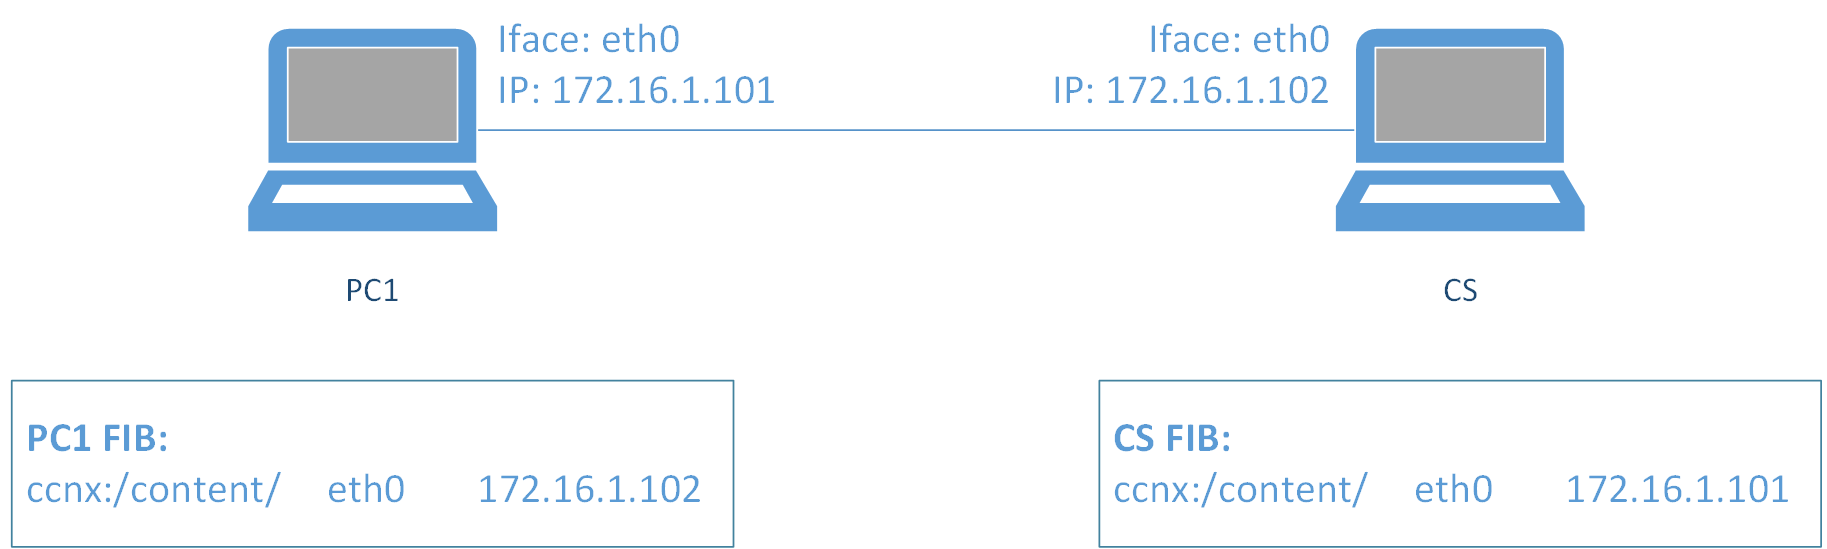
\includegraphics[width=0.80\textwidth]{figures/diag3.png}
    \cprotect\caption{Example of the configuration for Test 1. PC1 shall 
            execute \verb?ccncatchunks?, while CS executes \verb?ccnsendchunks?.}
    \label{fig:test-1-1}

\end{figure}

As \verb+ccncatchunks2+ implements its own flow control mechanism, the FIBs of 
both CCNx nodes are configured to route packets over UDP (see 
Section~\ref{subsubsec:fibs} for details), in order to avoid interference 
from TCP's own flow control. The content used for 
exchange in the tests consists in randomly generated data files of 500\,kB, 
5\,MB and 50\,MB. The chunk size parameter of \verb+ccnsendchunks+ is tested 
under three different values: 1024 byte, 4096 byte and 8192 byte.\vertbreak

The following parameters are measured:

\begin{enumerate}
    \item Throughput;
    \item Number of packets exchanged between ENs, discriminated by type;
    \item Bytes exchanged between ENs;
    \item Other parameters specific to \verb+ccncatchunks2+ flow control 
        mechanism.
\end{enumerate} 

Parameters 1, 2 and 3 from the above list shall be measured on a non-CCNx 
setting, by transferring data over FTP. The same setup shown 
in Figure~\ref{fig:test-1-1} is used, with CS running an FTP server 
(\verb?proftpd?\,\footnote{Available at \url{http://www.proftpd.org/}}) and PC1 
fetching content using an FTP client. Again, the content to be exchanged in the 
tests consists in the same randomly generated data files used in the CCNx tests.\vertbreak

\subsection{Test 2.1 - CCNx Multihop Forwarding (File Transfer)}
\label{subsec:test-multihop-file}

Here we test CCNx on the testbed scenario depicted in 
Figure~\ref{fig:basic-testbed}. The objective is to monitor network parameters as 
CCNx routers (INs) forward Interest and Data packets to\slash from a content source (CS) and 
two content consumers (PC1 and PC2), both sending Interests for the same 
content.\vertbreak

The same type of content as that used in Test 1 is used, but 
limited to a 5\,MB file\,\cprotect\footnote{\label{foot:note1}Preliminary tests with larger files (e.g. 50\,MB) 
have been conducted, however since \verb+ccnd+ keeps its cache in memory and 
due to issues in the cache replacement mechanism of OpenWRT's \verb+ccnd+, the 
RAM of the Linksys WRT160NL would exhaust quickly forcing a system restart.}. 
In this case, the \verb+ccnr+ application is used at CS to host a CCNx file 
repository, while PC1 and PC2 retrieve the file using \verb+ccngetfile+. Two 
subtypes of test are conducted: (1) PC1 and PC2 start the 
file transfer separately in time, i.e. PC2 starts releasing Interest packets 
after PC1 receives its last Data packet; and (2) PC1 and PC2 content 
requests overlap. The integrity of the transmitted files is verified via an 
MD5 checksum, for all transfers.\vertbreak

The following parameters are measured:

\begin{enumerate}
    \item Network load (packets\slash sec) at the different interfaces of INs, over time;
    \item Number of packets exchanged between INs, discriminated by type;
    \item Bytes exchanged between INs;
    \item CPU and memory usage in each IN, over the transfer time.
\end{enumerate}

As packet sniffing tasks are now being conducted at constrained nodes, we use 
\verb+tcpdump+ with the \verb+-s 500+ option, i.e. set to capture the initial 500 byte 
of each packet. Despite the fact that not all packet information is saved, 500 
byte are enough to capture the CCN's headers, along with the headers of any 
underlying protocols, allowing us to correctly assess packets sizes\,\footnote{In addition to capture file size reductions, the number of packets dropped by the kernel has consistently been reduced to 0 in all experiments.}.\vertbreak

Parameters 1 to 4 from the above list shall be measured on a non-CCNx 
setting, by transferring data over FTP. The same testbed setup as that 
used for the CCNx case (shown 
in Figure~\ref{fig:basic-testbed}) is used, with CS running an FTP server 
(\verb?proftpd?) and both PC1 and PC2 fetching content using 
an FTP client, in a non-overlapping fashion. Again, the content to be exchanged 
in the tests consists in the same randomly generated data files used in the CCNx tests.\vertbreak

\subsection{Test 2.2 - CCNx Multihop Forwarding (Video Streaming)}

The scenario for this test is similar to that of Test 2.1, now using CCNx's 
VLC plugin to playback a video stored at CS instead of directly transferring 
a file.\vertbreak

PC1 and PC2 both start the playback of video content using CCNx's VLC plugin, in 
the manner shown in Section~\ref{subsubsection:disseminating-ccnx}. Just as in 
Test 2.1, both non-overlapping and non-overlapping test subtypes are ran. The 
same parameters as those measured in Test 2.1 are evaluated in this case.\vertbreak

A 
video of size 6.3 MB\,\textsuperscript{\ref{foot:note1}} and duration of 8 seconds 
is used in the test: although not 
a quantitative measurement, the qualitative assessment of the video playback is 
also given (e.g. occurrence of playback gaps, frame `freezing', etc.).

\subsection{Test 2.3 - CCNx Multihop Forwarding (Multiple Paths)}
\label{subsec:mult-path}

The objective of this test is to assess how CCNx forwards packets when 
multiple paths exist between content sources and consumers. To do so, we use 
a slight variation of the previous testbed setup, shown in 
Figure~\ref{fig:testbed-multiple-paths}.\vertbreak

\begin{figure}[h!]

    \centering
    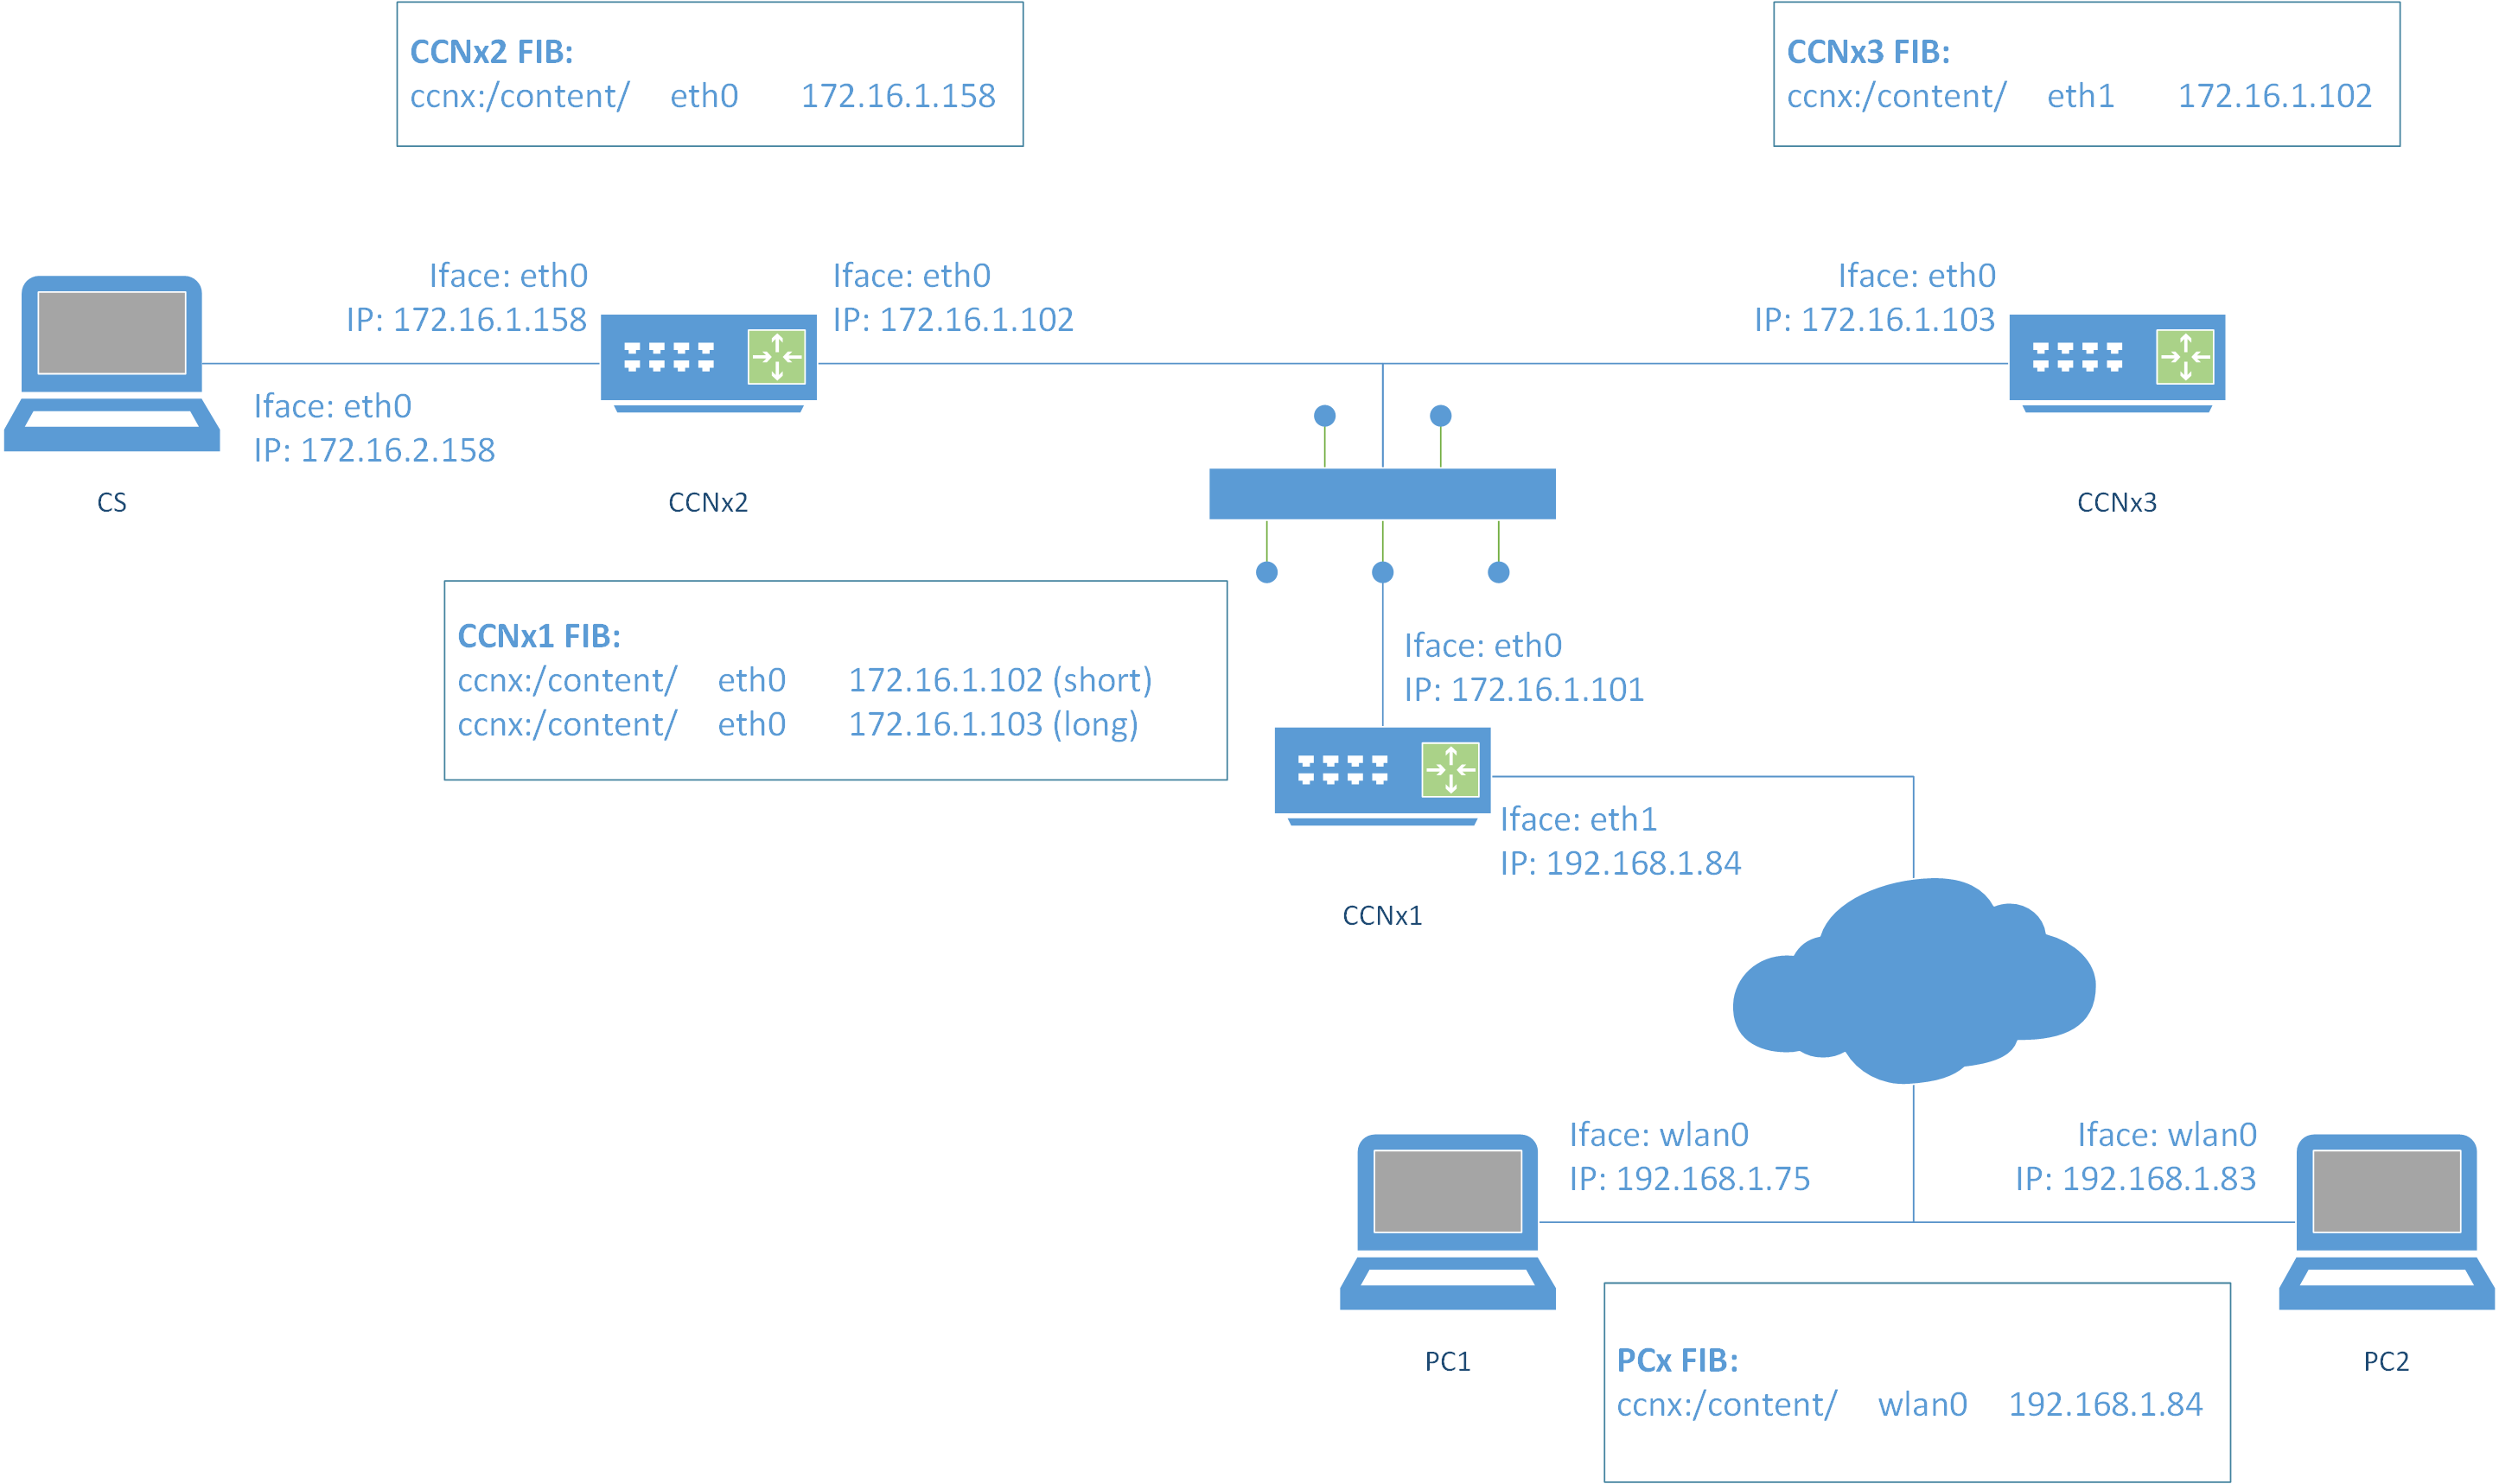
\includegraphics[width=0.80\textwidth]{figures/diag2.png}
    \cprotect\caption{Testbed arrangement for Test 2.3.}
    \label{fig:testbed-multiple-paths}

\end{figure}

The same type of content as that used in Test 2.1 (see 
Section~\ref{subsec:test-multihop-file}) is used, 
limited to a 5\,MB file. 
Again, the \verb+ccnr+ application is used at CS to host a CCNx file 
repository, while PC1 and PC2 retrieve the file using the \verb+ccngetfile+ 
application.\vertbreak 

Three subtypes of test are conducted: 

\begin{enumerate}

    \item PC1 and PC2 retrieve the content from CS via a short path, 
        via CCNx1 and CCNx2, in a non-overlapping fashion.
    \item PC1 and PC2 retrieve the content from CS via a long path, via 
        CCNx1, CCNx3 and CCNx2, in that order.
    \item PC1 and PC2 retrieve the content from CS with the INs configured 
        to forward packets via both short and long paths.

\end{enumerate}

The different paths are specified at the INs by adding manual entries to the 
FIB, using the \verb+ccndc+ command (see Section~\ref{subsubsec:fibs} for 
details). To test the influence of the order by which \verb+ccndc+ commands 
are ran, i.e. the order by which routing entries are put into the FIB, we 
first test a setting for which the `short path' is included first, followed 
by another setting for which the `long path' is included first. The same 
parameters as those measured in Tests 2.1 and 2.2 are evaluated in this case.


\chapter{Experimental Results}

Here we present the results from the tests specified in 
Section~\ref{sec:protocol}.\vertbreak

We present only part of the results in this chapter, as the complete 
setting of measurements is rather large considering the required 
length for this assignment. The complete 
collection of results can be consulted in Appendix~\ref{app:meas}.

\section{Test 1 - CCNx Throughput and Overhead}
\label{sec:res-throughput-overhead}

We choose the results for a representative case and elaborate on its 
discussion. The same reasoning and arguments can then be used to understand 
the remaining results shown in Appendix~\ref{app:meas}.

\begin{figure}[h!]

    \centering
    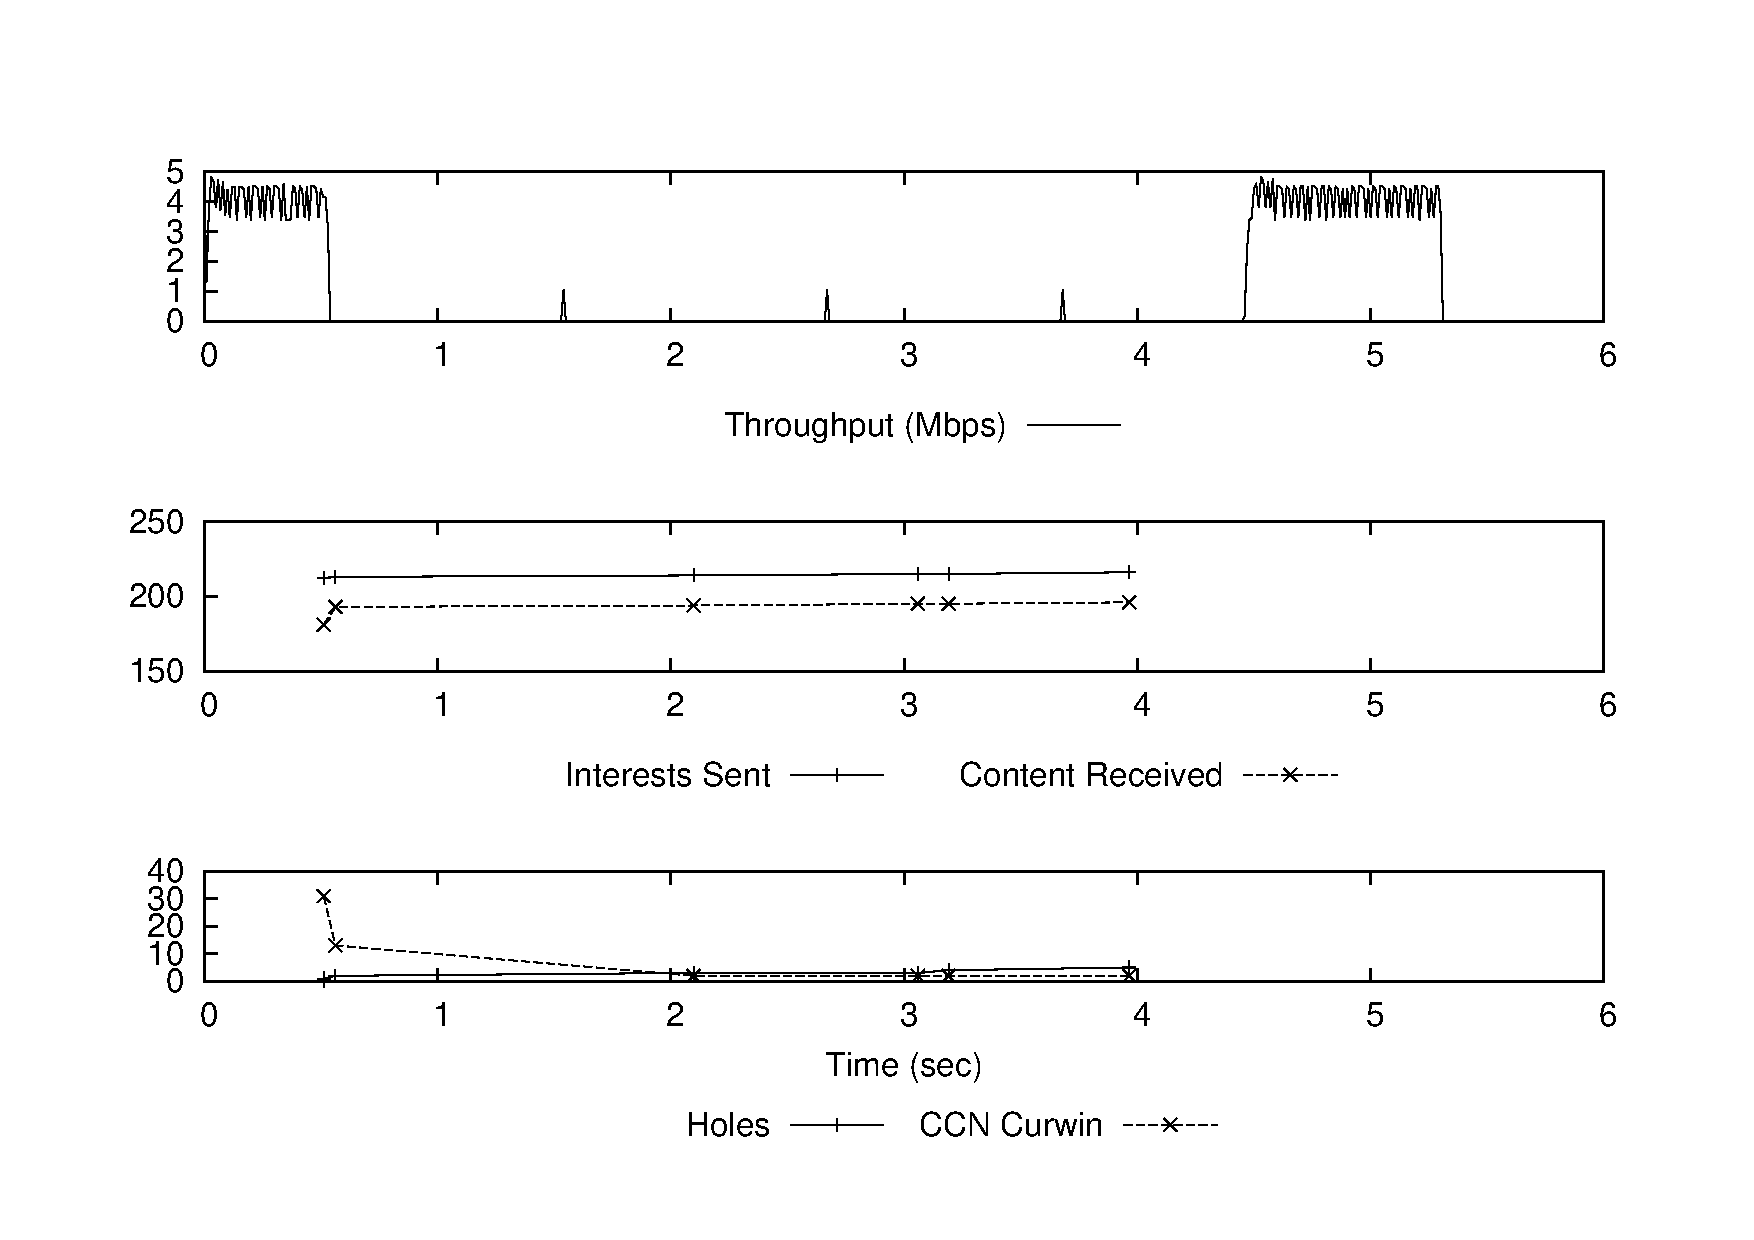
\includegraphics[width=0.75\textwidth]{figures/udp_0_5_1024.pdf}
    \cprotect\caption{Results for Test 1: Throughput in Mbps, as perceived by 
        PC1, when retrieving a file of size 500\,kB with a 1024 byte 
        `chunk' size.}
    \label{fig:test-1-thpt-0_5-1024}

\end{figure}

Figure~\ref{fig:test-1-thpt-0_5-1024} shows the results for the throughput and 
other CCNx specific statistics, as perceived by PC1, when retrieving a file of 
size 500\,kB with a 1024 byte `chunk' size. The action of the joint flow 
control mechanism applied by both \verb+ccncatchunks2+ and \verb+ccnsendchunks+ 
applications (introduced in Section~\ref{subsubsection:disseminating-ccnx}) is 
visible: note how after 0.5 seconds of transfer the throughput drops as well as 
the `Curwin' value (i.e. the size of the window\slash pipeline of Interests 
\verb+ccncatchunks2+ sends to \verb+ccnsendchunks+ at a time), which drops 
from 31 (the maximum size) to 1. Note that such an event is coincident with 
the occurrence of `holes', i.e. a lack of Interest-to-Data packet correspondence. 
After this point, small transferring peaks are visible after approx. 1 second 
intervals, once again consistent with the expected behavior of the 
\verb+ccnsendchunks+ application. This flow control mechanism has 
a severe impact on the overall goodput, i.e. the number of useful information 
bits over the total amount of time required for transfer (approx. 5.35 seconds).\vertbreak

\begin{figure}[h!]

    \centering
    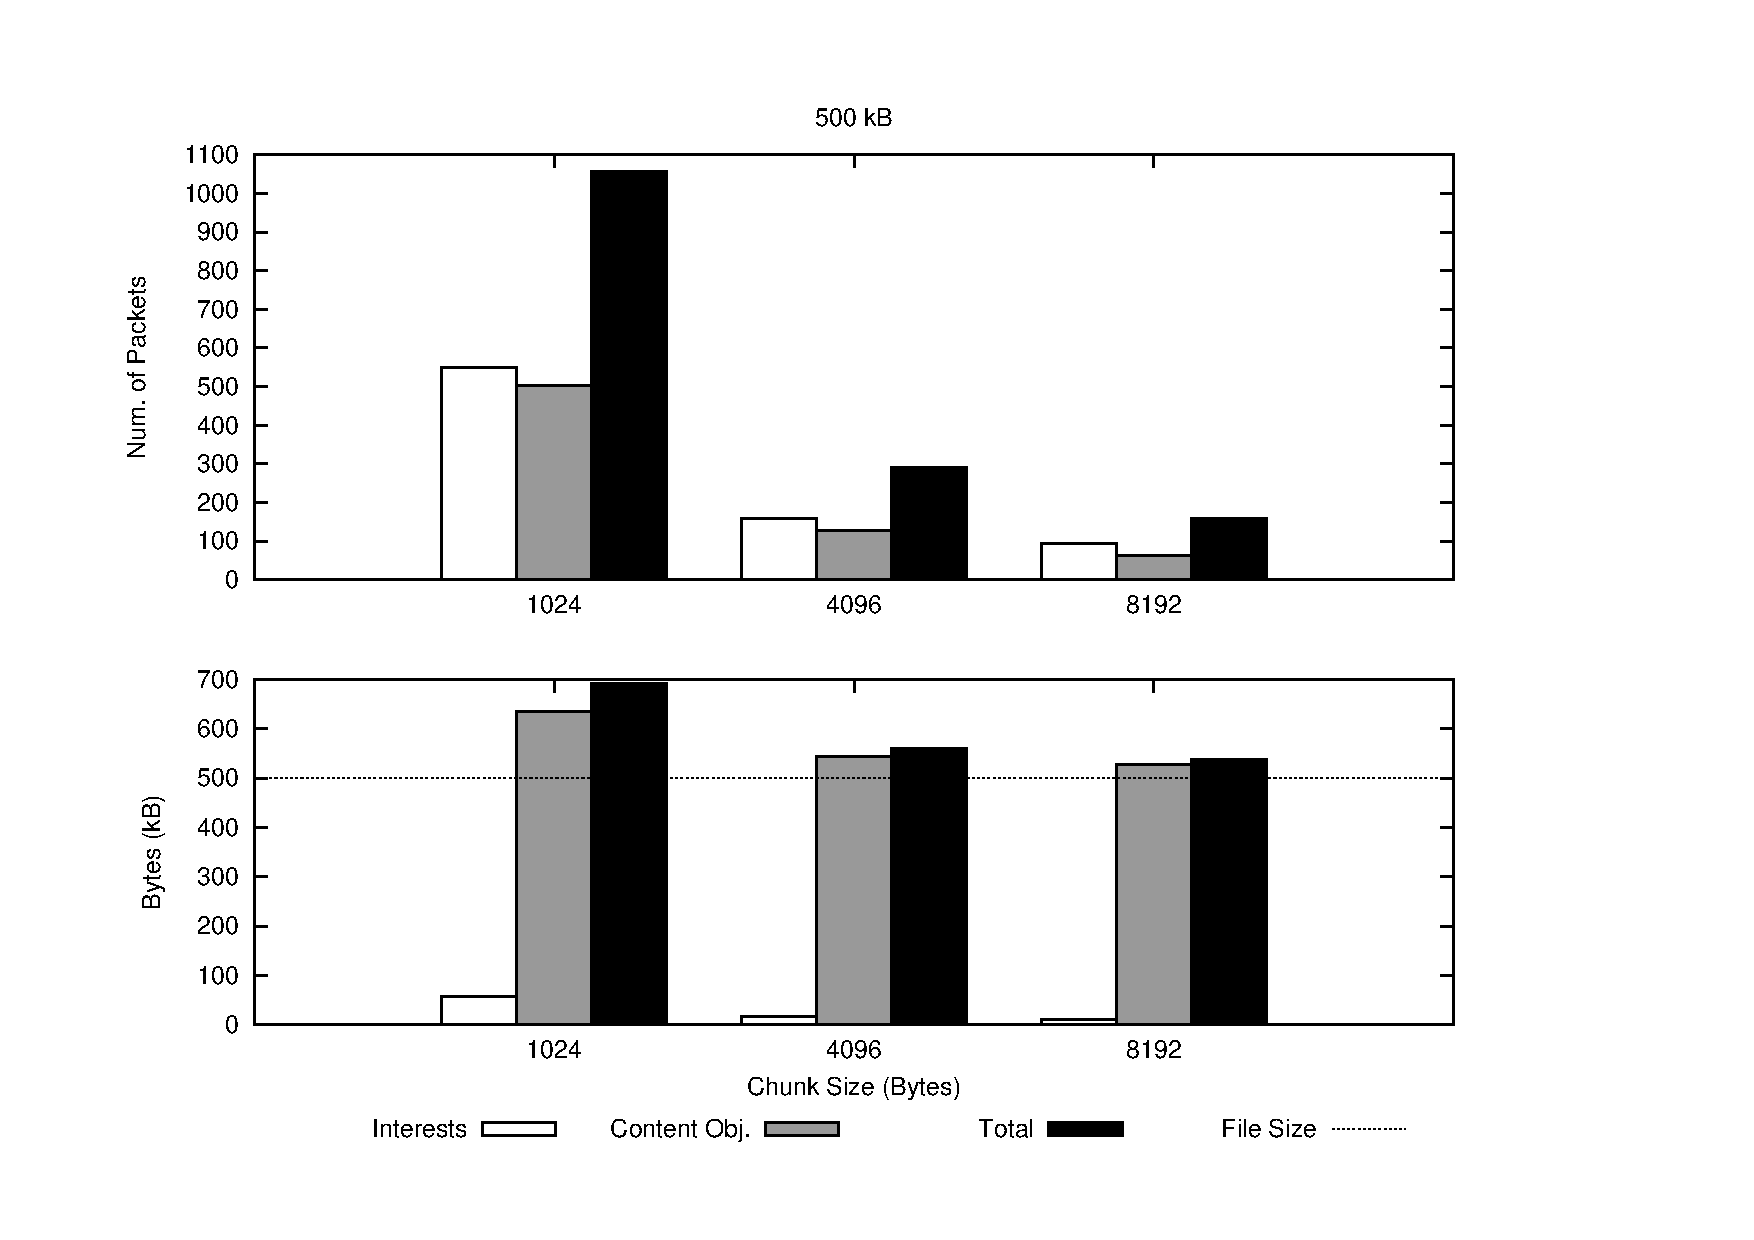
\includegraphics[width=0.75\textwidth]{figures/udp_0_5.pdf}
    \cprotect\caption{Results for Test 1: Packet and byte quantities, measured 
        at PC1, for a file size of 500\,kB.}
    \label{fig:test-1-packtes-bytes}

\end{figure}

Figure~\ref{fig:test-1-packtes-bytes} presents the results for the number of 
packets and bytes, as measured by the capture filters in PC1. Again, we include 
the results for a 500\,kB file size and a `chunk' size of 1024 byte. The amount 
of Interest packets consistently surpasses the amount 
of Data packets, for all `chunk' sizes. This is explained by the 
`loss' of a batch of $N$ pipelined Interest packets, due to overloading of the 
\verb+ccnsendchunks+ application. In the case of 500\,kB, e.g. for a `chunk' 
size of 1024 byte, one can situate the mismatch between Interest and Content 
Objects (or Data packets) within the interval $]0;100]$. This is consistent 
with the results shown in Figure~\ref{fig:test-1-thpt-0_5-1024}, with the 
mismatch being equal to the sum of values of `Curwin', at the time of 
occurrence of `hole' events.\vertbreak

\begin{figure}[h!]

    \centering
    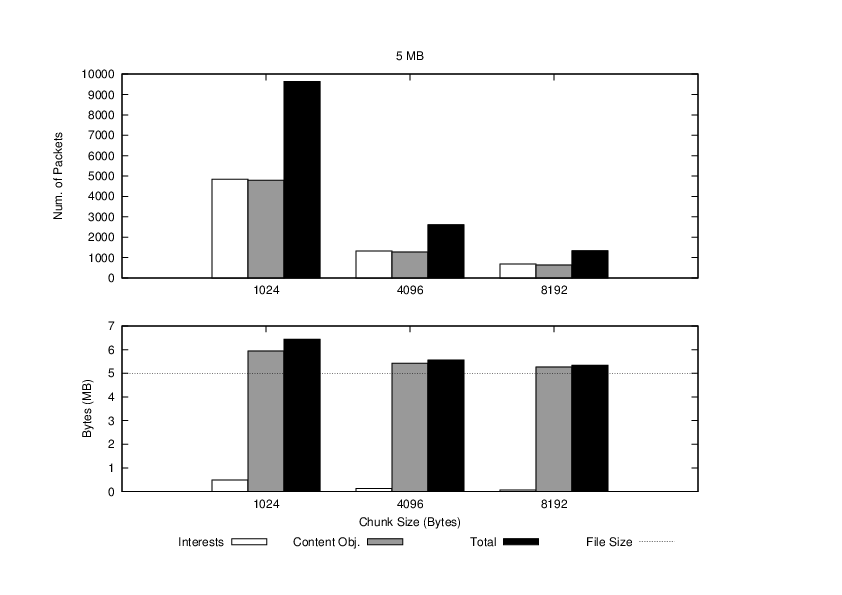
\includegraphics[width=0.75\textwidth]{figures/udp_5.pdf}
    \cprotect\caption{Results for Test 1: Packet and byte quantities, measured 
        at PC1, for a file size of 5\,MB.}
    \label{fig:test-1-packtes-bytes-5}

\end{figure}

\begin{figure}[h!]
    \centering

    \subfigure[]{
        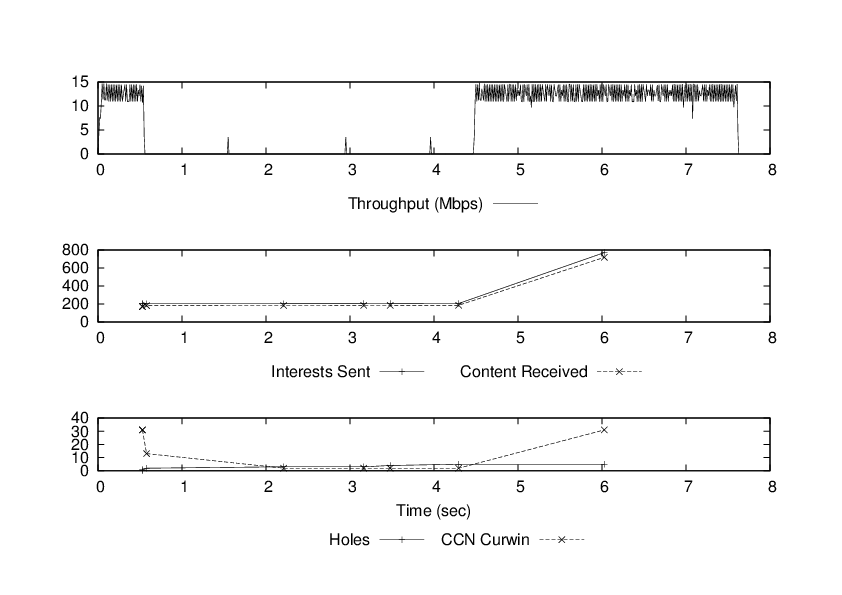
\includegraphics[width=0.75\textwidth] {figures/udp_5_4096.pdf}
        \label{subfig:udp_5_4096}
    }

    \subfigure[]{
        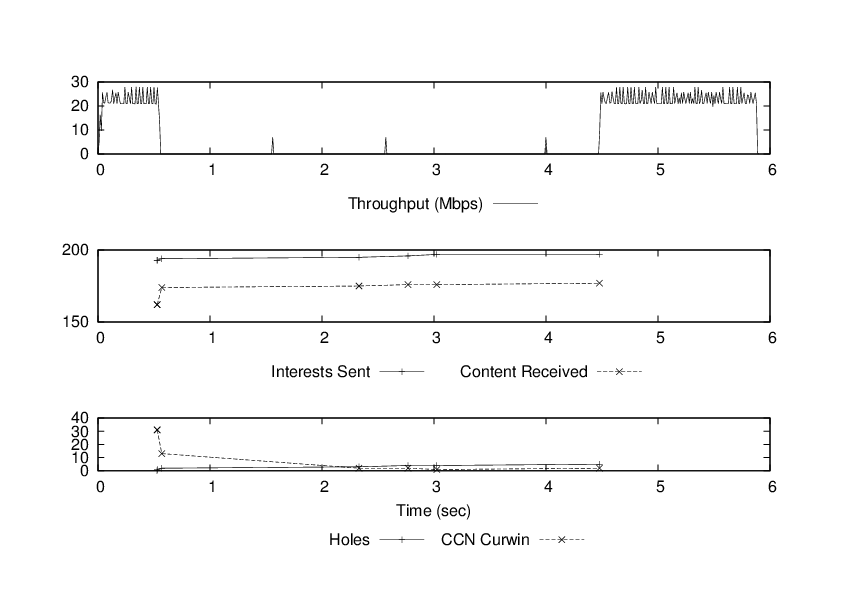
\includegraphics[width=0.75\textwidth] {figures/udp_5_8192.pdf}
        \label{subfig:udp_5_8192}
    }

    \cprotect\caption{Results for Test 1: Throughput in Mbps, as perceived by 
        PC1, when retrieving a file of size 5\,MB with 4096 and 8192 byte 
        `chunk' sizes.}
    \label{fig:udp_5}

\end{figure}

We consider the results for the file size of 5\,MB, depicted in 
Figures~\ref{fig:udp_5} and~\ref{fig:test-1-packtes-bytes-5}, to further 
elaborate on CCNx throughput and overhead. 
In order to easily visualize the impact of the variation of `chunk' size in 
overhead, we have added an horizontal line on the byte quantity charts in 
Figure~\ref{fig:test-1-packtes-bytes-5}, equal to the respective file 
size.\vertbreak 

The difference between the quantity of Content Object bytes and the 
file size decreases as the `chunk' size increases, i.e. the overhead decreases 
with the increase of the chunk size. This can be explained by several 
factors, identified by examining the packet 
capture logs:

\begin{itemize}

    \item The header of a CCNx Content Object, is composed 
        by the following fields (consistent with the Data packet
        descriptions given in Section~\ref{sec:ccn-packets}), resulting in a 
        total max. of 215 byte:

        \begin{enumerate}

            \item Type of packet code (2 byte)
            \item CCN signature (128 byte)
            \item Content name codified as ASCII (32 to 35 byte)
            \item Signed information (50 byte)

        \end{enumerate}

    \item CCNx (at least \verb+ccnsendchunks+ in particular) relies on IP 
        fragmentation to transport Content Object packets with data fields (i.e. 
        payloads) larger than 1480 byte, which is in turn related with the 
        maximum size allowed for a standard Ethernet frame, 1518 byte.

\end{itemize}

So in the case of `chunk' sizes $C$ of 1024 byte, for every 1024 byte of data 
there is an 
additional $~$\,220 byte\,\footnote{By verification of the capture logs, the 
only variable field is the content name, regardless of the `chunk' size.}, while 
in the case of $C = 4096$ or $8192$ byte that header is `spread' over larger 
payload sizes, reducing the overhead. Nevertheless, the overhead of CCNx may 
then be effectively set at 188 byte plus the size of the content name string.\vertbreak

Regarding Figure~\ref{fig:udp_5}, the throughput increases with the 
`chunk' size as well. By verification of the packet capture logs, the throughput 
limitations are imposed by the rate of generation of 
Content Objects and not by the rate at which Interest packets are sent 
(maybe due to the signature generations for each content block 
by part of the \verb+ccnsendchunks+ application\,\footnote{See the discussion 
in \url{https://www.ccnx.org/pipermail/ccnx-dev/2010-April/000188.html}.}), as 
for all file sizes and `chunk' sizes, the average inter-packet arrival times 
for Content Objects (in periods where the throughput is maximum) are 
approximately the same, $\sim$\,2.5 milliseconds. Considering the sizes of 
Content Objects for each 
`chunk' size (including CCNx header), we have the following estimates for 
throughput values, consistent with the values shown in 
Figures~\ref{fig:test-1-thpt-0_5-1024} and~\ref{fig:udp_5}:

\begin{itemize}

    \item 1024 byte: $\frac{1}{0.0025} \times (1024 + 220) \times 8 \approx 3.98$\,Mbps
    \item 4096 byte: $\frac{1}{0.0025} \times (4096 + 220) \times 8 \approx 13.8$\,Mbps
    \item 8192 byte: $\frac{1}{0.0025} \times (8192 + 220) \times 8 \approx 26.9$\,Mbps

\end{itemize}

The results for the non-CCN case, obtained by fetching the same files via FTP 
are shown in Appendix~\ref{app:meas}, in Section~\ref{app:res-throughput-overhead}. As expected, 
the use of channel bandwidth is much more efficient 
(approaching throughput values of Fast Ethernet's 100\,Mbps) as well as lower values of 
overhead. In terms of packet numbers, as FTP avoids payload sizes larger than 
1416 byte (so that frames do not exceed Ethernet’s MTU of 1500 byte), the packet counts 
are (compared with the number of Content Objects) larger.

\section{Test 2 - CCNx Multihop Forwarding}
\label{sec:res-multihop-for}

We now present the results for the CCNx multihop forwarding tests, described 
in Section~\ref{sec:protocol}. We divide the presentation of the results by 
subtype, i.e. the results for Tests 2.1, 2.2 and 2.3 are presented individually.

\subsection{Test 2.1 - CCNx Multihop Forwarding (File Transfer)}
\label{subsec:test-multihop-file-res}

Figure~\ref{fig:file_5-net} depicts the network load (in packets per 
second) at each of the CCNx nodes 
in the testbed (see Figure~\ref{fig:basic-testbed}), for both non-overlapping and 
overlapping file retrieval cases. A 5\,MB file is retrieved via a wireless 
link between CCNx node (IN) CCNx3 and ENs PC1 and PC2. The CCNx 
routes established for this test follow those specified in Figure~\ref{fig:basic-testbed}.\vertbreak

\begin{figure}[h!]
    \centering

    \subfigure[]{
        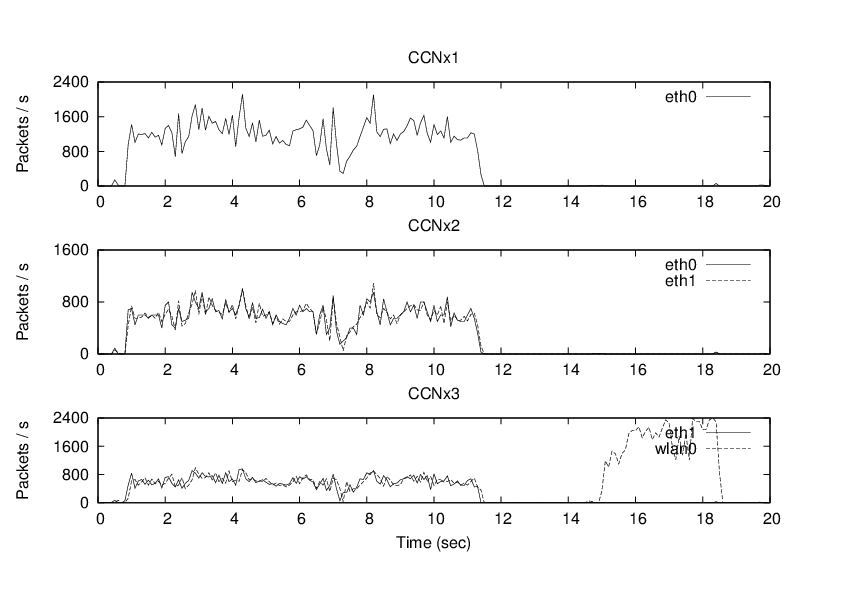
\includegraphics[width=0.75\textwidth] {figures/file_5-sep-net.pdf}
        \label{subfig:file_5-sep-net}
    }

    \subfigure[]{
        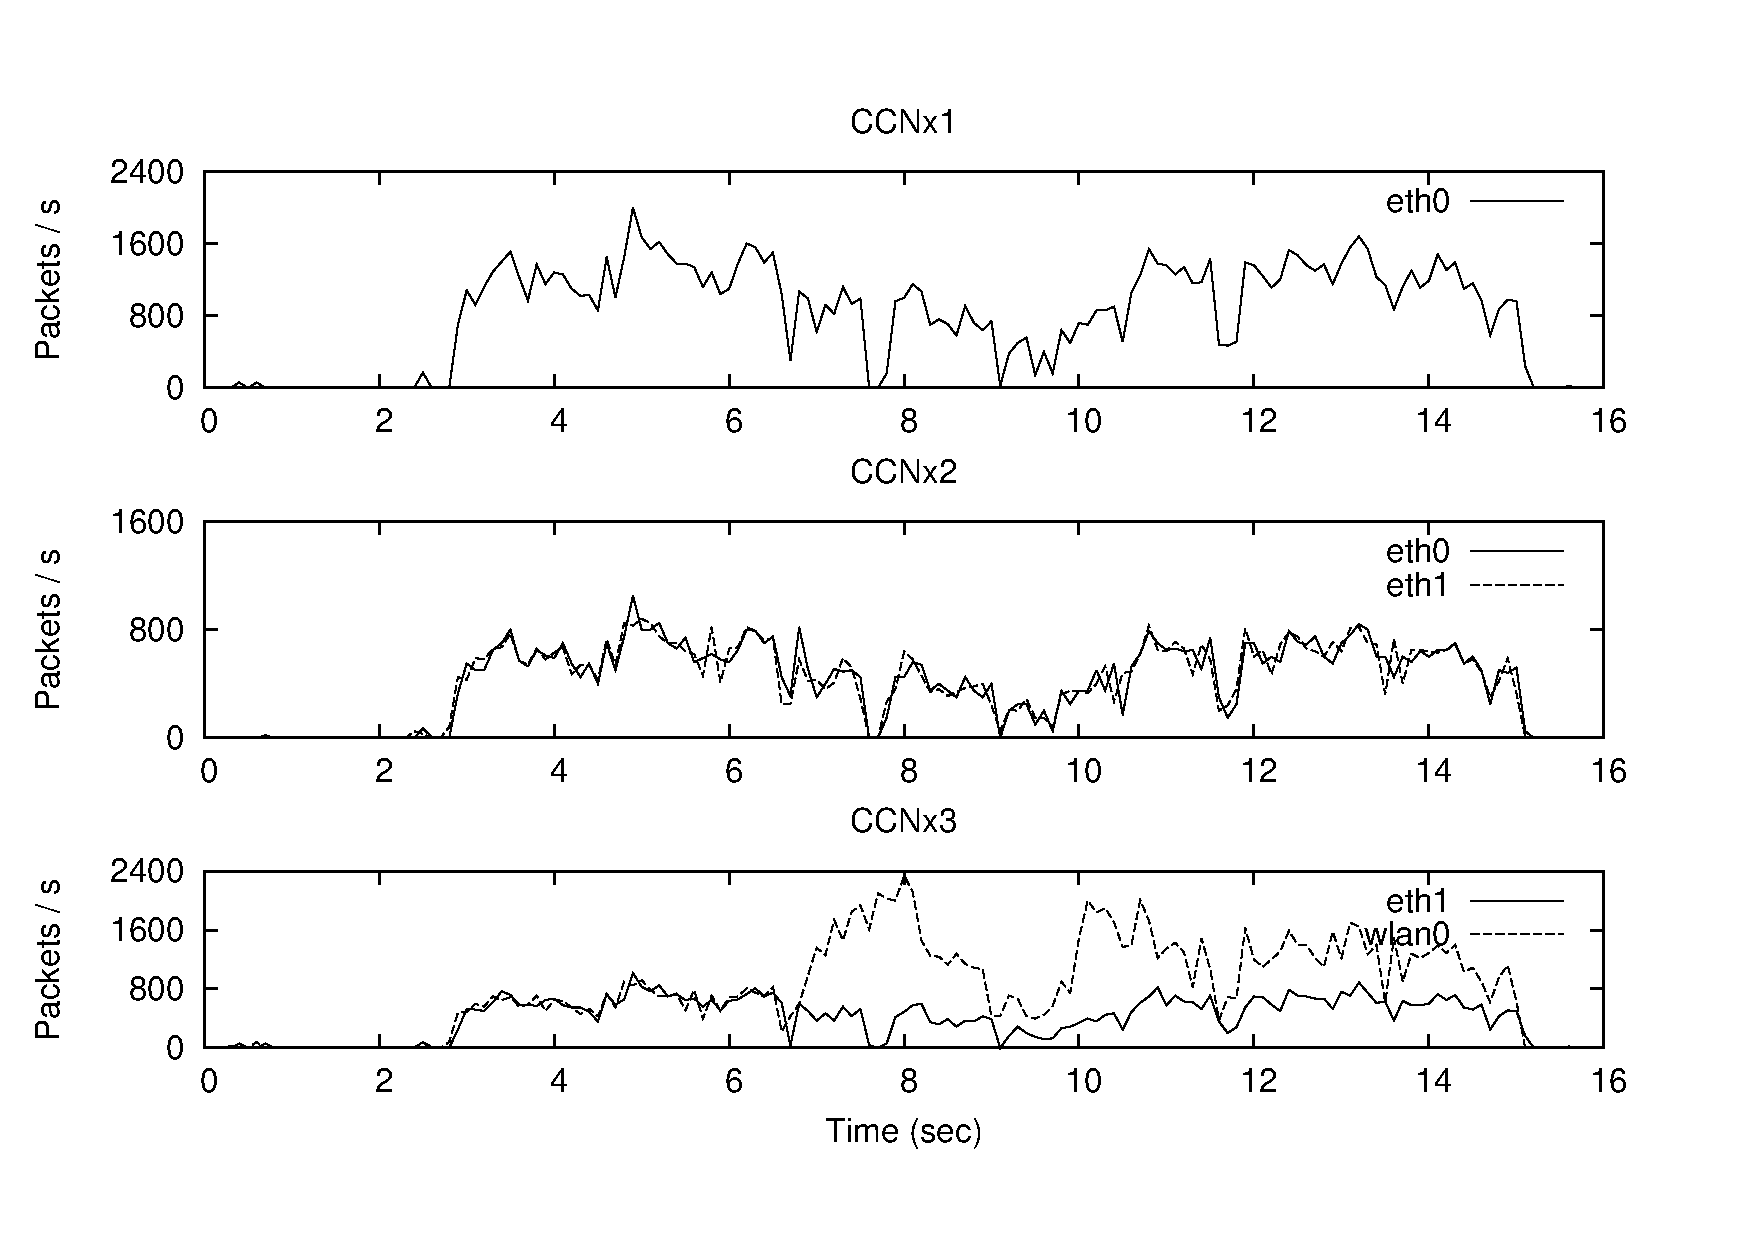
\includegraphics[width=0.75\textwidth] {figures/file_5-sim-net.pdf}
        \label{subfig:file_5-sim-net}
    }

    \cprotect\caption{Results for Test 2.1: Network load, in packets per 
        second, as perceived by each of the CCNx nodes in the testbed, 
        while PC1 and PC2 retrieve a file of size 5\,MB via a wireless 
        link, through CCNx3. The graph in (a) shows the results for 
        the non-overlapping file retrieval, while (b) shows the 
        overlapping case.}
    \label{fig:file_5-net}

\end{figure}

In Figure~\ref{subfig:file_5-sep-net} the effect of CCN's in-network caching 
characteristic is perfectly noticeable: the load on CCNx3 shows two clear 
activity clusters, one for the initial retrieval of the file by PC1, which 
extends for approx. 11 seconds and another for the file retrieval 
by part of PC2, which takes approx. 3 seconds. During the initial period, the 
remaining CCNx nodes display a similar activity pattern, corresponding to 
the forwarding of Interest and Data packets between the several CCNx hops, up 
to the CS node. The values for CCNx1 seem doubled when compared to the other 
nodes, since the forwarding is made via a single interface, \verb+eth0+. The 
second period only shows activity on CCNx1, as expected, as PC2 is 
retrieving the content cached in CCNx1's Content Store. The transfer is 
also clearly faster than in the initial retrieval, as no intermediate CCNx 
forwarders exist between content publisher and subscriber.\vertbreak

In Figure~\ref{subfig:file_5-sim-net}, the load values 
on CCNx3 are similar on both interfaces \verb+eth1+ and \verb+wlan0+, up 
until approx. 7 seconds from the start of the test. At this point, a spike 
on the load for interface \verb+wlan0+ is verified, corresponding to the 
entry of PC2. For an initial period (7 to 8 seconds) PC2 retrieves the 
content already cached at CCNx3, while for the remaining time the Data packets 
arriving at CCNx3 from interface \verb+eth1+ are multicasted to both 
PC1 and PC2. Figure~\ref{fig:file_5-pckt-counts} shows that in terms of 
packet counts --- Interests and Data packets --- there is no difference between 
the overlapping and non-overlapping cases.\vertbreak

\begin{figure}[h!]
    \centering

    \subfigure[]{
        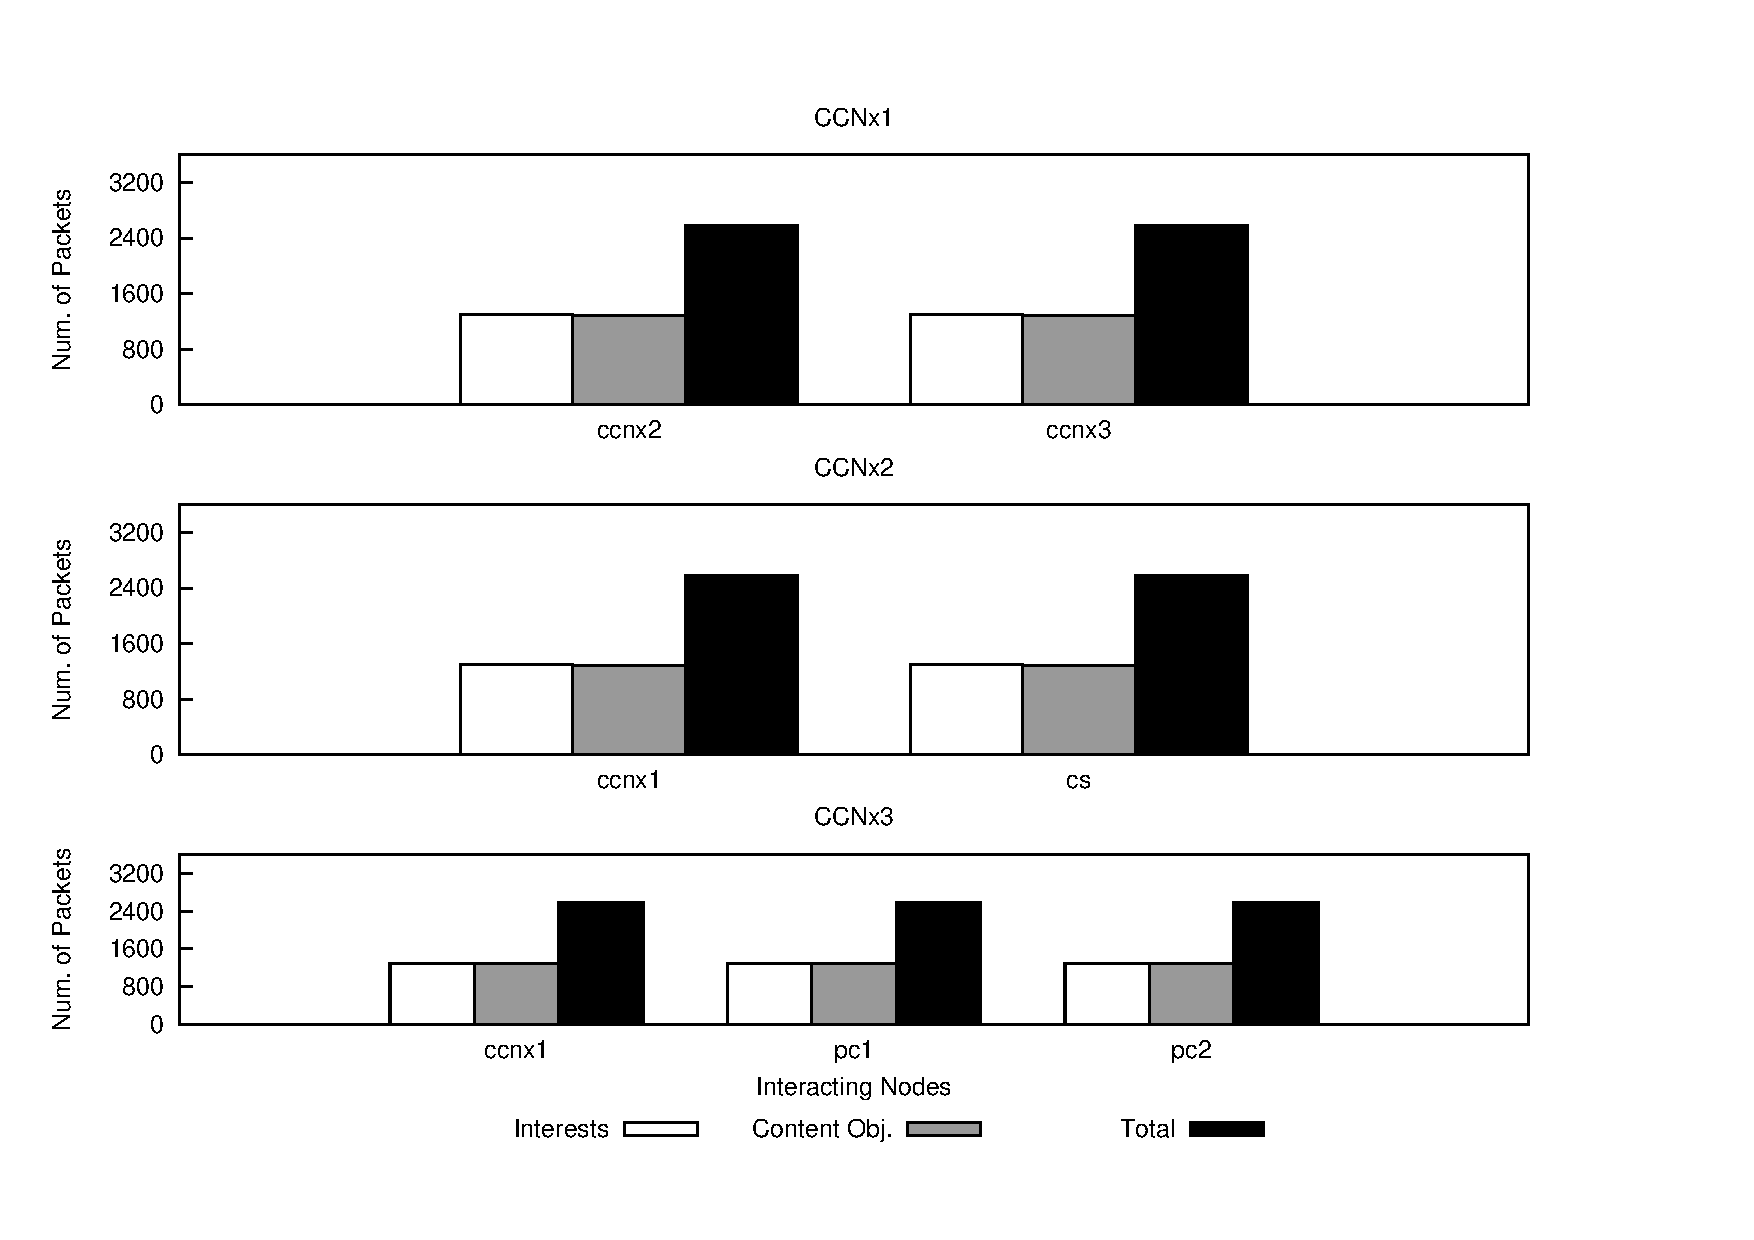
\includegraphics[width=0.75\textwidth] {figures/file_5-sep-pckt.pdf}
        \label{subfig:file_5-sep-pckt}
    }

    \subfigure[]{
        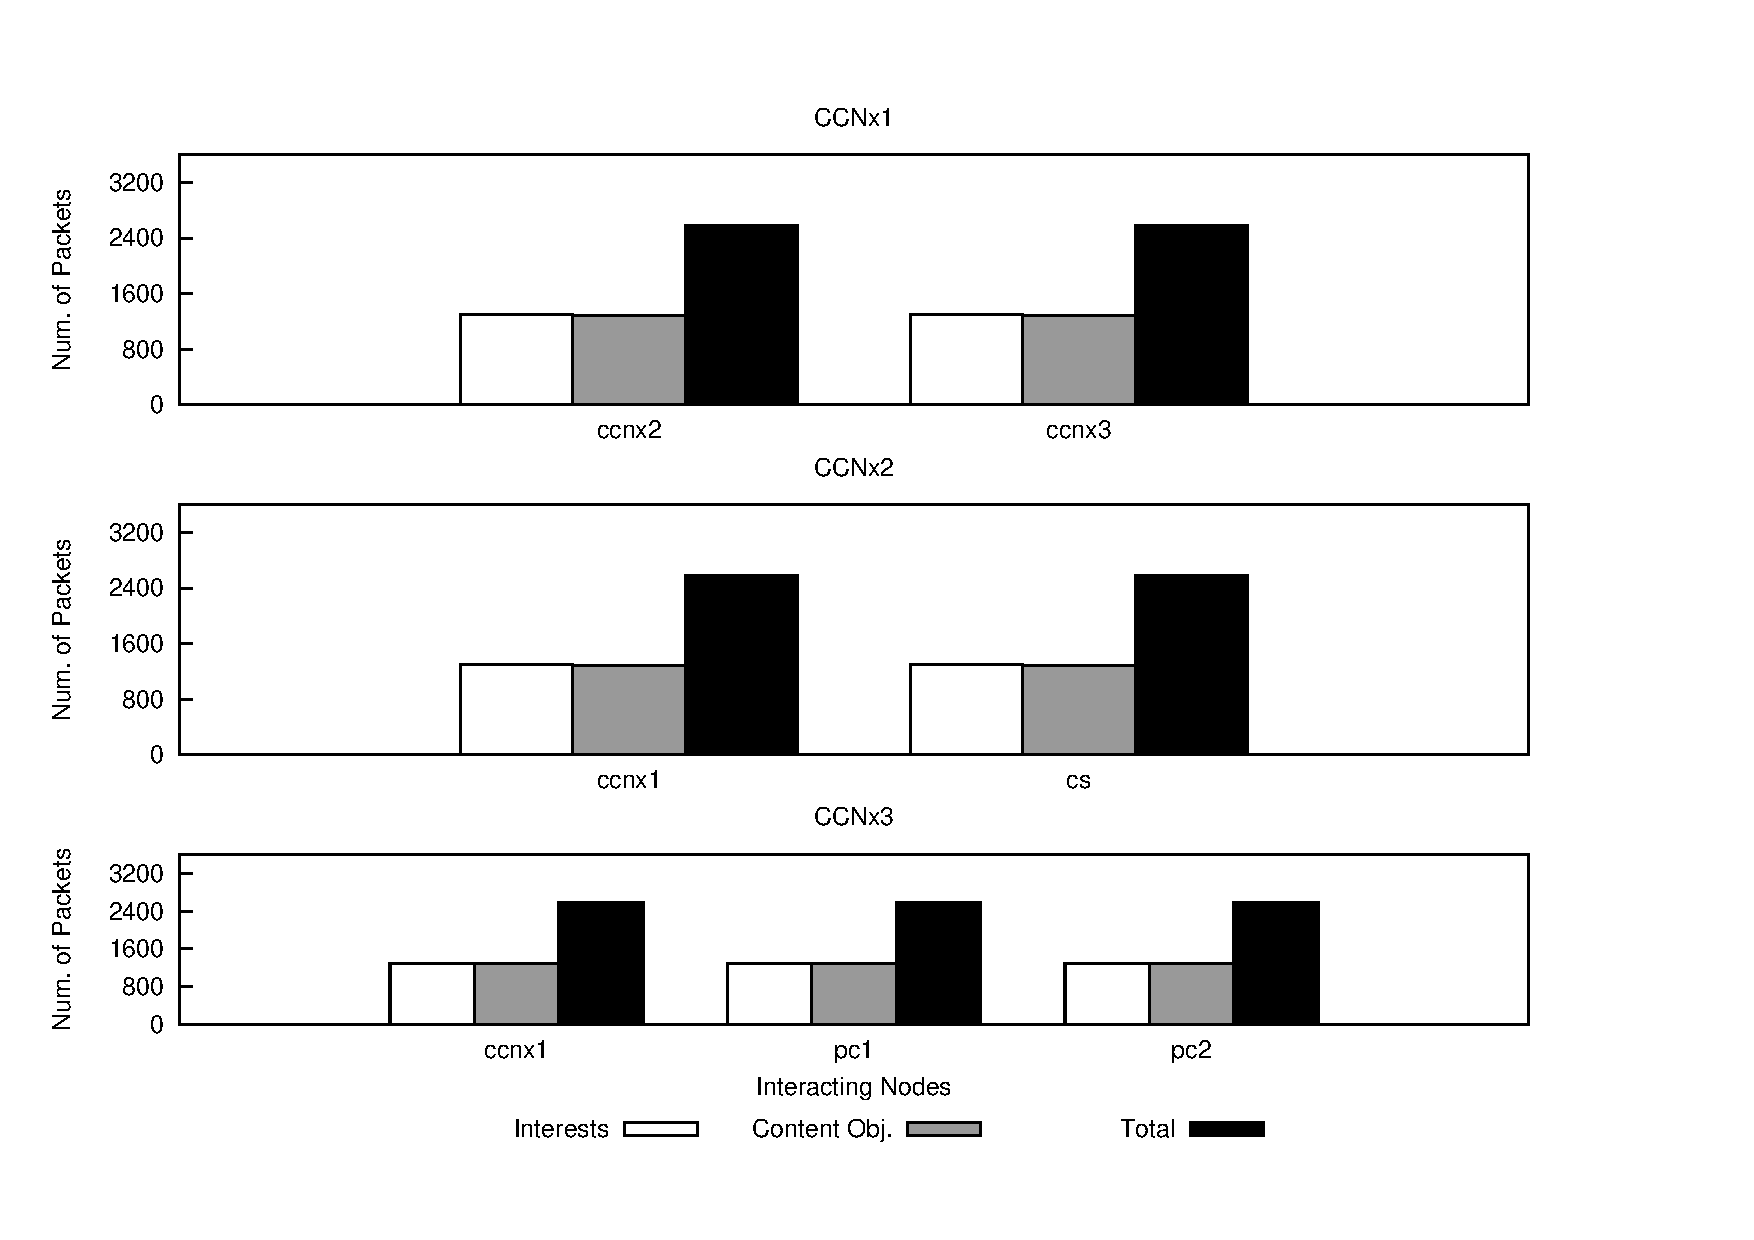
\includegraphics[width=0.75\textwidth] {figures/file-sim-pckt.pdf}
        \label{subfig:file-sim-pckt}
    }

    \cprotect\caption{Results for Test 2.1: Packet counts (Interest and 
        Content Objects) registered at each CCNx forwarding node, exchanged 
        between the respective peer elements. Case (a) presents the results 
        for the non-overlapping case, while (b) shows the results for the 
        overlapping case.}
    \label{fig:file_5-pckt-counts}

\end{figure}

The remaining test cases and results for Test 2.1 can be consulted in 
Appendix~\ref{app:meas}, in Section~\ref{subapp:test-multihop-file}.

\subsection{Test 2.2 - CCNx Multihop Forwarding (Video Streaming)}
\label{subsec:test-multihop-video}

We now present the results for Test 2.2 in Figure~\ref{fig:video-sep-net}. We 
limit the presented results to the network load values at each of the CCNx 
nodes, leaving the remaining measurements to Appendix~\ref{app:meas}.\vertbreak

Similarly to the file transfer results shown in 
Section~\ref{subsec:test-multihop-file-res}, Figure~\ref{subfig:video-sep-net} 
shows two separate network activity clusters: (1) up until approx. 14 seconds 
for the streaming to PC1 and (2) from approx. 17 till 25.5 seconds for the 
streaming to PC2. In terms of time length, (1) clearly exceeds the time 
duration of the video used as sample, which was reflected by several gaps 
in the video playback. In the case of (2) such gaps were still noticed, but 
not as frequent or as long.\vertbreak

\begin{figure}[h!]
    \centering

    \subfigure[]{
        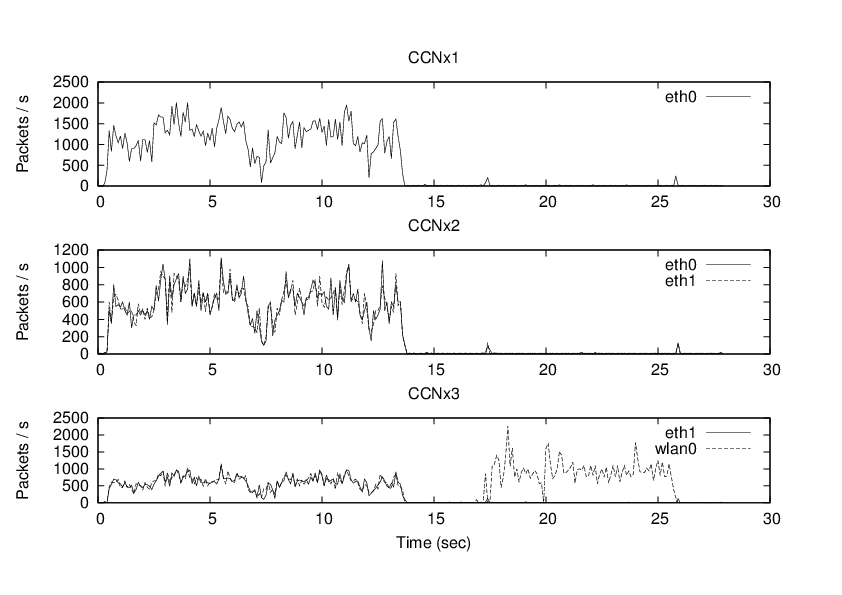
\includegraphics[width=0.75\textwidth] {figures/video-sep-net.pdf}
        \label{subfig:video-sep-net}
    }

    \subfigure[]{
        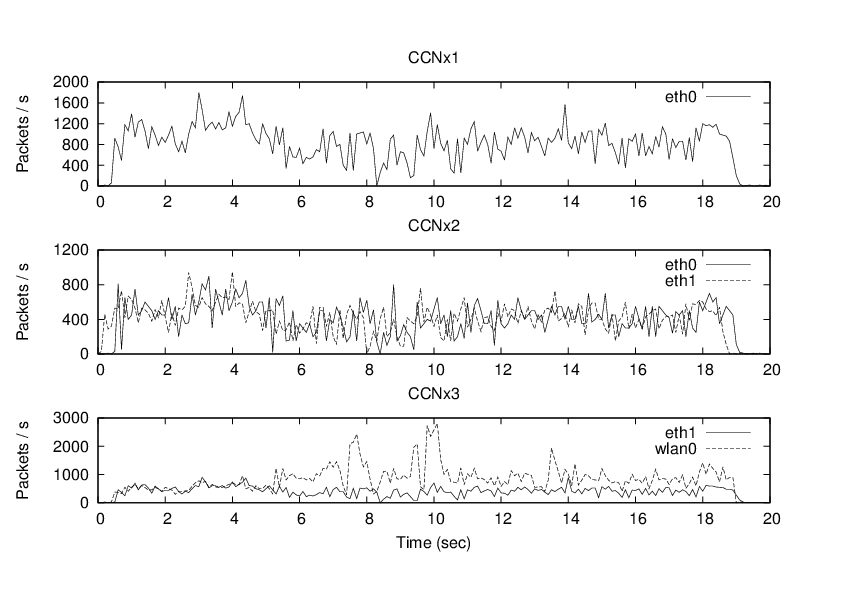
\includegraphics[width=0.75\textwidth] {figures/video-sim-net.pdf}
        \label{subfig:video-sim-net}
    }

    \cprotect\caption{Results for Test 2.2: Network load, in packets per 
        second, as perceived by each of the CCNx nodes in the testbed, 
        while PC1 and PC2 playback a streamed video file of size 6.3\,MB 
        and 8 second duration, via a wireless 
        link, through CCNx3. The graph in (a) shows the results for 
        the non-overlapping streaming case, while (b) shows the 
        overlapping case.}
    \label{fig:video-sep-net}

\end{figure}

In the case of Figure~\ref{subfig:video-sim-net}, again similar results 
to that of Test 2.1 were verified, including a spike in the values of the load 
at CCNx3's \verb+wlan0+ interface upon the initialization of PC2's streaming 
activity, at around 5 seconds after the initialization of the test. Again, the 
time length for the video download is extended, now reflected by frequent gaps 
in the video playback.\vertbreak

\begin{figure}[h!]

    \centering
    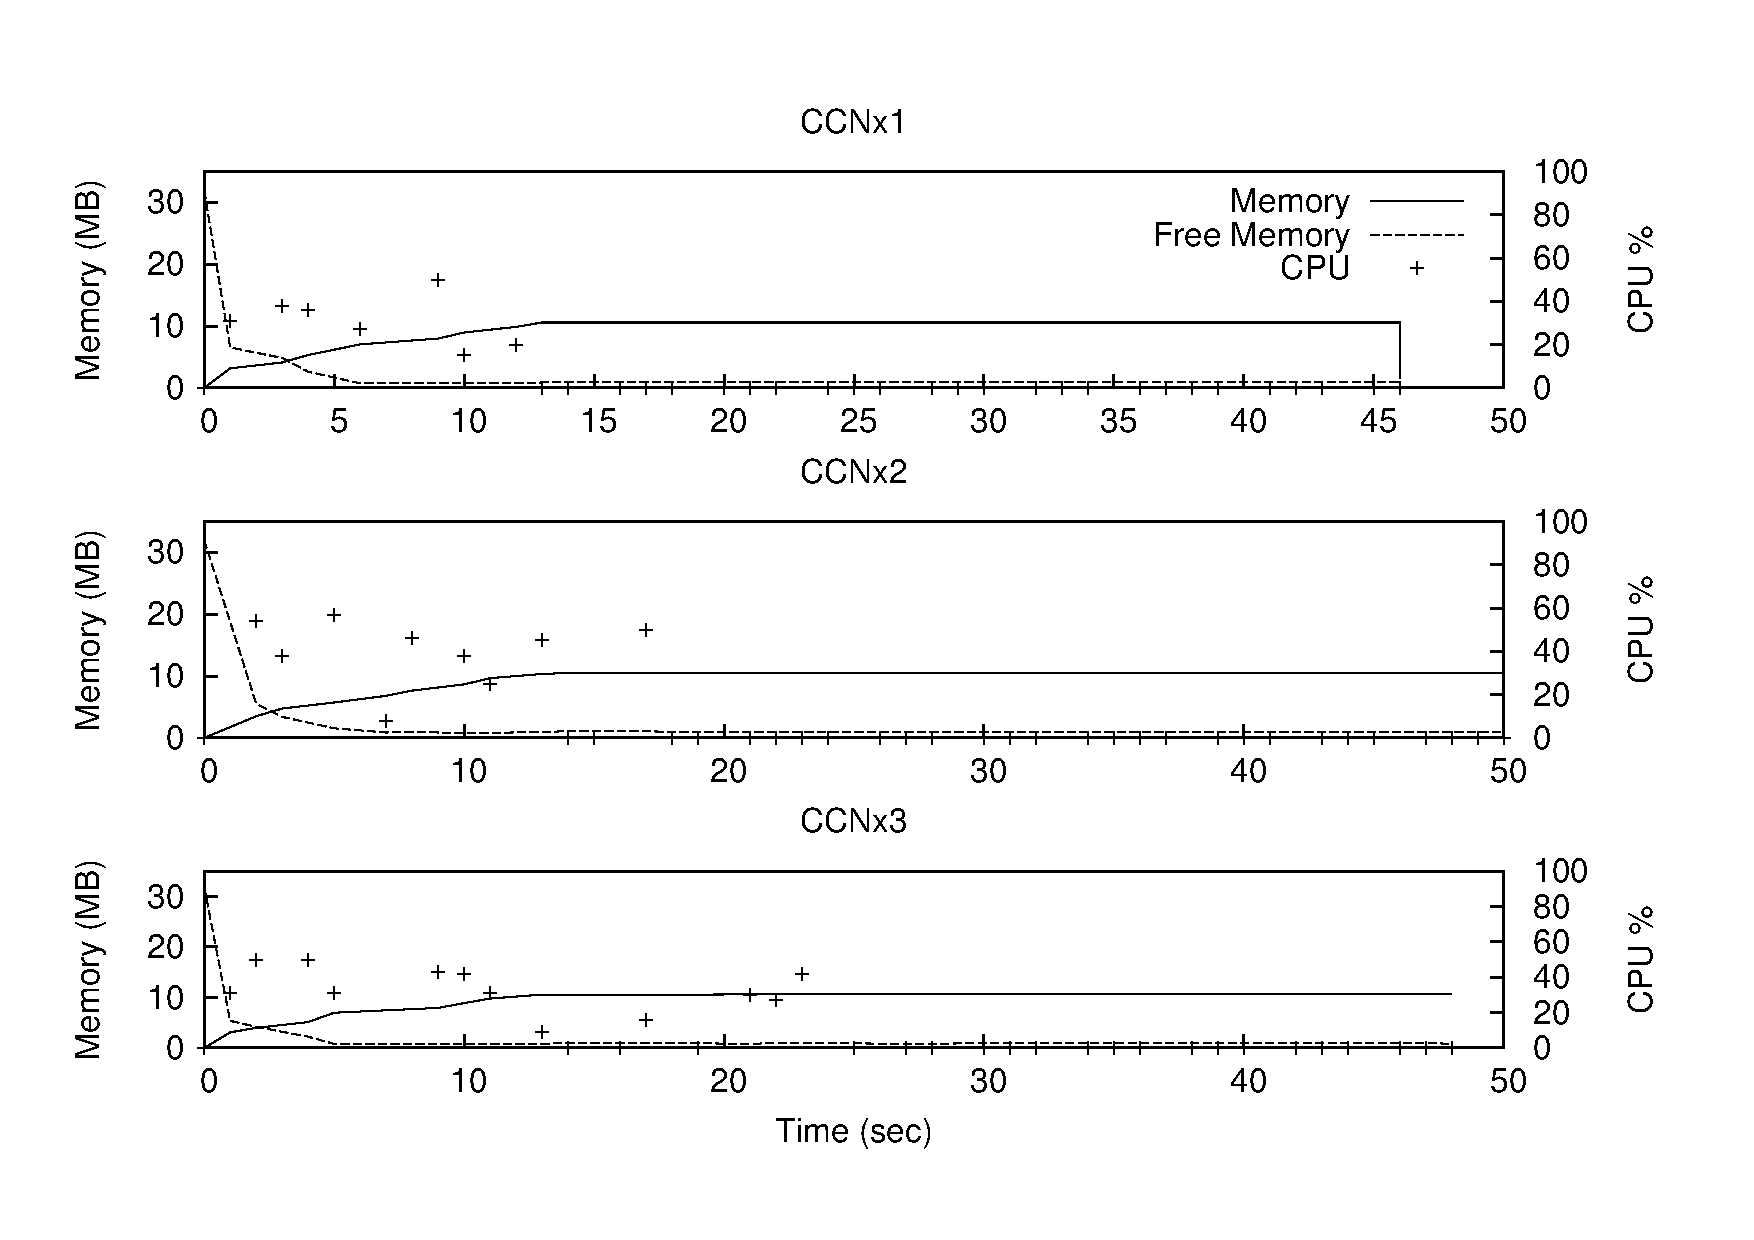
\includegraphics[width=0.75\textwidth]{figures/video-sep-cpu-mem.pdf}
    \cprotect\caption{Results for Test 2.2: CPU and memory utilization at 
        all CCNx nodes, during the streaming of a video file of size 
        6.3\,MB and 8 second duration, non-overlapping case. Regarding the 
        memory values, the `memory' line corresponds to the amount of RAM 
        occupied by the \verb+ccnd+ process, while the `free memory' corresponds 
        to the amount of free memory in the system.}
    \label{fig:video-sep-cpu-mem}

\end{figure}

Figure~\ref{fig:video-sep-cpu-mem} shows the values of CPU and memory 
consumption for the non-overlapping test case. The `memory' line corresponds 
to the amount of RAM used by the CCNx's main process, \verb+ccnd+. It is clear 
how the memory usage increases as the content of the video file is forwarded 
among the CCNx nodes, stabilizing at approx. 14 seconds after the test
 initialization, at the same time the transfer with PC1 is finished. Even though 
these measurements evaluate more the implementation of CCNx than the 
CCN concept itself, these highlight a need for efficient cache 
replacement policies and CCNx applications for constrained devices such as 
the routers used in this experiment. Although for general use cases, CCN nodes 
such as home gateways may have caching disabled, for experimental applications 
such as CCNx applied to Vehicular Networks (VANETS)~\cite{Amadeo2013,Grassi2013}, these 
concerns should be taken into account.

\subsection{Test 2.3 - CCNx Multihop Forwarding (Multiple Paths)}
\label{subsec:test-multihop-multipath}

In the case of the multiple path scenario presented in 
Section~\ref{subsec:mult-path}, we show the results for the packet counts 
registered at each CCNx forwarding node, as the load values are similar to 
those of the non-overlapping version of Test 2.1. Other measurements not 
shown here may be consulted in Appendix~\ref{app:meas}, 
Section~\ref{subapp:test-multihop-multipath}.\vertbreak

Figure~\ref{subfig:long-route} shows the packet counts (Interest and 
Content Objects) registered at each CCNx forwarding node, exchanged 
between the respective peer elements, in this case for the `long' route 
only.\vertbreak 

A note should be 
made to help distinguish the origin of Interest and Content Object packets in the 
chart, which is related to the way the routes are established among 
nodes (see Figure~\ref{fig:testbed-multiple-paths}): e.g. for CCNx1 the value 
of Interest packets associated with `PC1' and `PC2' represents those 
\textit{received} from PC1 and PC2, while the quantity associated with `CCNx3' 
represents the number of Interests \textit{forwarded} to CCNx3. The same 
reasoning can be applied to the Content Objects: those associated with 
`PC1' and `PC2' are \textit{forwarded} to these nodes, while the values associated 
with `CCNx3' correspond to the Content Objects \textit{received} from CCNx3.\vertbreak

The values in Figure~\ref{subfig:long-route} are expected, with no 
divergences between the number of forwarded packets between each of the 
INs and ENs. Furthermore, the existence of a single path (or 
conversely the absence of the `short' path) is noticed by the 
absence of values associated with CCNx2 and CCNx1 for nodes CCNx1 and CCNx2, 
respectively.\vertbreak

\begin{figure}[h!]
    \centering

    \subfigure[]{
        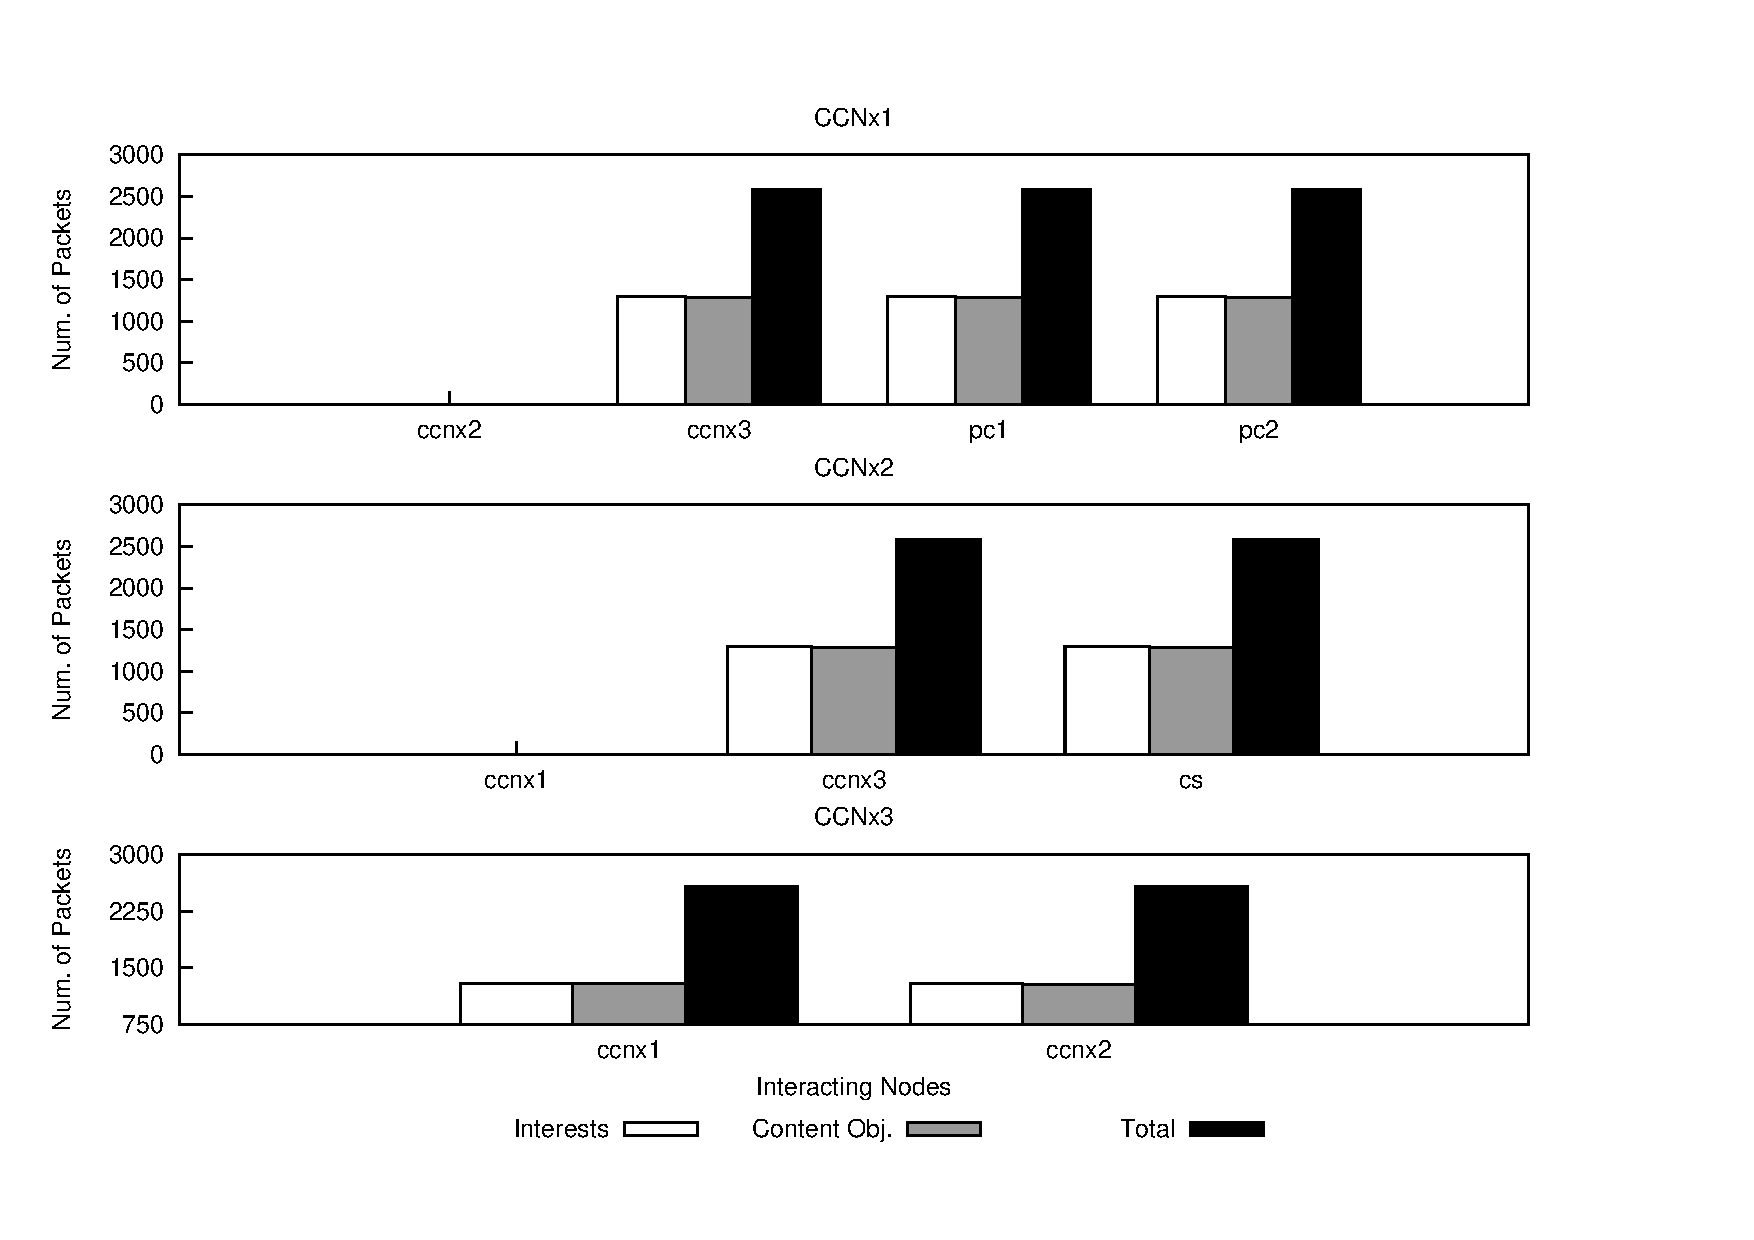
\includegraphics[width=0.75\textwidth] {figures/long-route.pdf}
        \label{subfig:long-route}
    }

    \subfigure[]{
        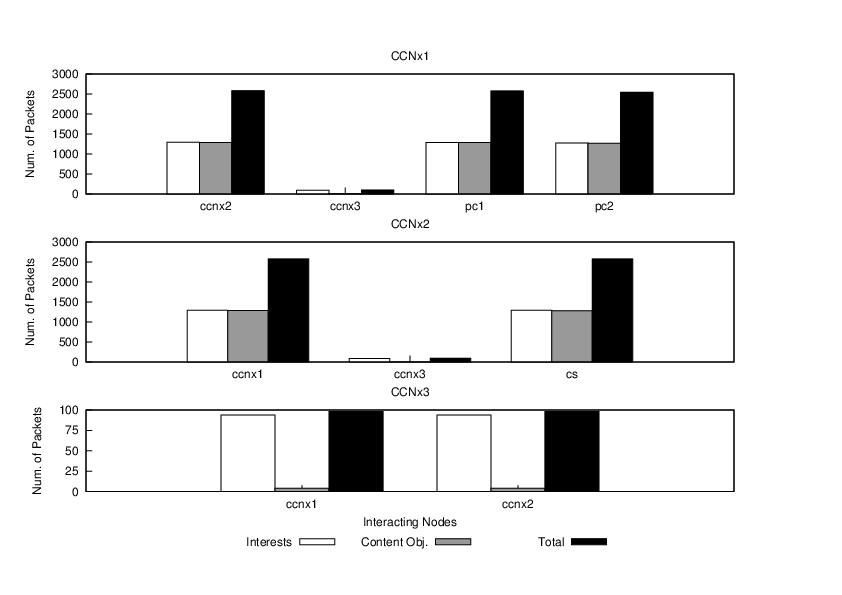
\includegraphics[width=0.75\textwidth] {figures/long-short-route.pdf}
        \label{subfig:long-short-route}
    }

    \cprotect\caption{Results for Test 2.3: Packet counts (Interest and 
        Content Objects) registered at each CCNx forwarding node, exchanged 
        between the respective peer elements. Case (a) presents the results 
        for the `long' route only, while (b) shows the results for multiple 
        paths, i.e. with the junction of both `long' and `short' routes.}
    \label{fig:routes-pckt-counts}

\end{figure}

In the case of Figure~\ref{subfig:long-short-route}, the presence of multiple 
paths is visible by the amount of Interest packets which are forwarded along 
the `long' path, i.e. from CCNx1 to CCNx3 and then from CCNx3 to CCNx2. From 
consultation of the capture logs, one verifies that a small quantity of 
Interest packets ($\sim 90$) is forwarded by CCNx1 to both CCNx2 and CCNx3. 
Only a residual number of Content Objects is forwarded by 
CCNx2 to CCNx3, corresponding to special CCNx packets exchanged among peers, 
not directly related to the content being requested by PC1 and PC2 (these 
pertain to `probing' Interest packets, periodically sent along alternative 
interfaces in order to detect better paths~\cite{Yi2013}). As the 
Interests forwarded by CCNx3 to CCNx2 are duplicated (arriving after those 
issued by CCNx1), these are discarded by CCNx2.


\chapter{Conclusions}

This work provided an introduction to the inner workings of a particular ICN 
approach via experimentation with CCN's open source implementation Project 
CCNx.\vertbreak

We have tested CCNx by mounting and running several experiments over a simple 
testbed of constrained devices (low CPU power and memory capabilities). We 
verify that a direct application of CCNx to such device types is not feasible, 
considering the test cases presented here.\vertbreak

As future work, since Web Caches and CCNx both at rather high layers of the 
network stack (implementing a similar functionality) it could be interesting to 
compare the performance of CCNx against the use of intermediate Web Caches. 
Tests with a modified version of the \verb+ccnchat+ application may prove 
useful for evaluating exchange patterns with small and sporadic messages, the 
scenario often found in M2M, WSNs or VANETS.\vertbreak

The results and insights provided by this work can prove useful for alterations 
of CCNx at both conceptual (e.g. alternatives to the transport mechanisms 
provided by \verb+ccncatchunks2+) and implementation (e.g. throughput limits 
imposed by \verb+ccnsendchunks+) levels, specially when regarding the 
application of CCNx to applications using constrained devices.

%-----------------------------------------------------------
%\addcontentsline{toc}{chapter}{\numberline{}Bibliography}
%\include{biblio}
\bibliographystyle{unsrt}
\bibliography{dsn,dsn-non-paper}
%-----------------------------------------------------------
\appendix
\chapter{CCNx Quick Reference}
\label{app:ccnx-specificss}

Here we provide a quick reference for several CCNx commands and applications 
used in this work. We follow a similar section structure as that of 
Section~\ref{subsec:ccnx-specifics}.

\section{CCNx Forwarding Tables}

To add a route allowing a node \verb+ccnx1+ to forward Interest packets 
directed at content domain \verb+ccnx:/content/files/+, the following 
\verb+ccndc+ command shall be used:

\begin{verbatim}
user@ccnx1:-# ccndc add ccnx:/content/files/ udp 172.16.1.101
\end{verbatim}

This command will tell \verb+ccnd+ to forward any Interests for content matching 
the prefix \verb+ccnx:/content/files/+ to the IP address 172.16.1.101, over UDP.

\section{Disseminating Content with CCNx}

\cprotect\subsection{Usage of \verb+ccnr+ and \verb+ccngetfile+}

In CCNx, content sources use a specific repository application for storing 
content and make it available in CCNx networks by responding to 
matching Interests, \verb+ccnr+~\cite{website:ccnx-commands}. The following 
sequence of commands initializes a repository and inserts a file into it, 
making it addressable via the name \verb+ccnx:/CCN_REPO_DIR/file1.dat+:

\begin{verbatim}
user@cs:-# ccnr
user@cs:-# ccnputfile ccnx:/CCN_REPO_DIR/file1.dat file1.dat
\end{verbatim}

The 
\verb+ccngetfile+ application~\cite{website:ccnx-commands} 
can then be used to release Interest packets to the CCNx network, querying 
for particular content, e.g. (assuming that 
\verb+CCN_REPO_DIR+ = \verb+/content/files+):

\begin{verbatim}
user@ccnx1:-# ccngetfile ccnx:/content/files/file1.dat file1.dat.local
\end{verbatim}

The command above releases Interests for the content 
\verb+ccnx:/content/files/file1.dat+ and saves the file locally as 
\verb+file1.dat.local+. Being a CCNx application, it follows CCN's `1 Data packet 
per Interest' principle~\cite{Jacobson2009}, but with pipelining of Interests, 
i.e. the application immediately releases $N$ Interest packets into the network 
before the actual reception of Data packets. The actual behavior of this 
exchange (flow control) is analyzed in some of the tests specified in 
Section~\ref{sec:protocol}.

\cprotect\subsection{Usage of \verb+ccnsendchunks+ and \verb+ccncatchunks2+}

We provide examples of the use 
of both commands below, for an exchange of content 
\verb+ccnx:/content/files/file1.dat+ between nodes \verb+ccnx1+ (sender) 
and \verb+ccnx2+ (receiver):

\begin{verbatim}

user@ccnx1:-# ccnsendchunks -b 4096 ccnx:/content/files/file1.dat < file1.dat.ccnx1

(...)

user@ccnx2:-# ccncatchunks2 -p 31 ccnx:/content/files/file1.dat > file1.dat.ccnx2

\end{verbatim}

With the combination of commands shown above, \verb+ccnx1+ gets ready to 
send Data packets, each one containing blocks of 4096 bytes of the 
file \verb+file1.dat.ccnx1+. This content may be addressed via 
the content name \verb+ccnx:/content/files/file1.dat+. On the other end, 
\verb+ccnx2+ starts sending batches of (at most) 31 Interest packets for the 
content \verb+ccnx:/content/files/file1.dat+, saving the file as 
\verb+file1.dat.ccnx2+ when all the chunks are finally transmitted.

\cprotect\subsection{Usage of VLC plugin}

E.g. for reproducing some content addressed 
as \verb+ccnx:/content/files/video.avi+, located somewhere in the 
networks, VLC should be called in the following way (note the triple slash `\slash'):

\begin{verbatim}

user@ccnx1:-# vlc ccnx:///content/files/video.avi

\end{verbatim}

\chapter{Additional Measurements}
\label{app:meas}

\section{Test 1 - CCNx Throughput and Overhead}
\label{app:res-throughput-overhead}

\begin{figure}[H]

    \centering
    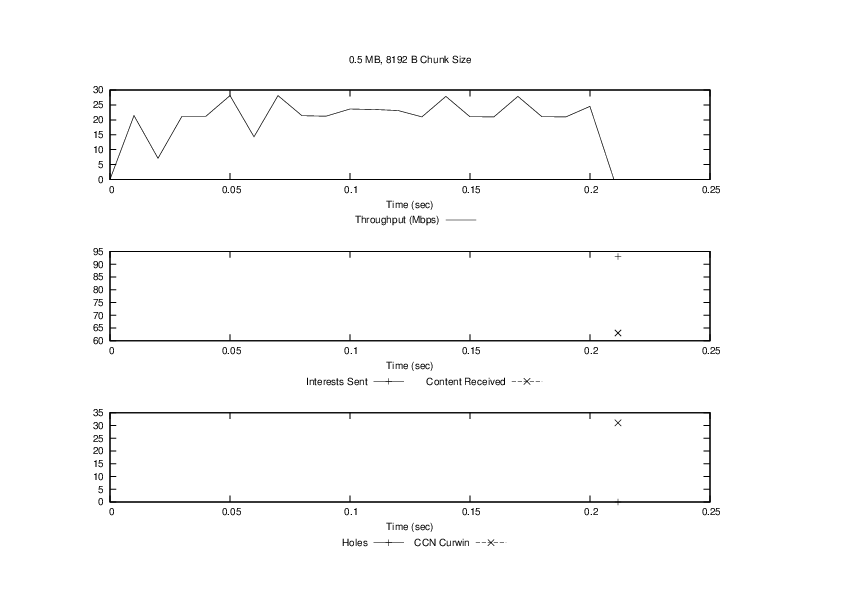
\includegraphics[width=0.75\textwidth]{figures/udp_0_5_8192.pdf}
    \cprotect\caption{Results for Test 1: Throughput in Mbps, as perceived by 
        PC1, when retrieving a file of size 500\,kB with a 8192 byte 
        `chunk' size. Statistics specific to the \verb+ccncatchunks2+ application 
        are also shown.}
    \label{fig:test-1-thpt-0_5-8192}

\end{figure}

\begin{figure}[H]

    \centering
    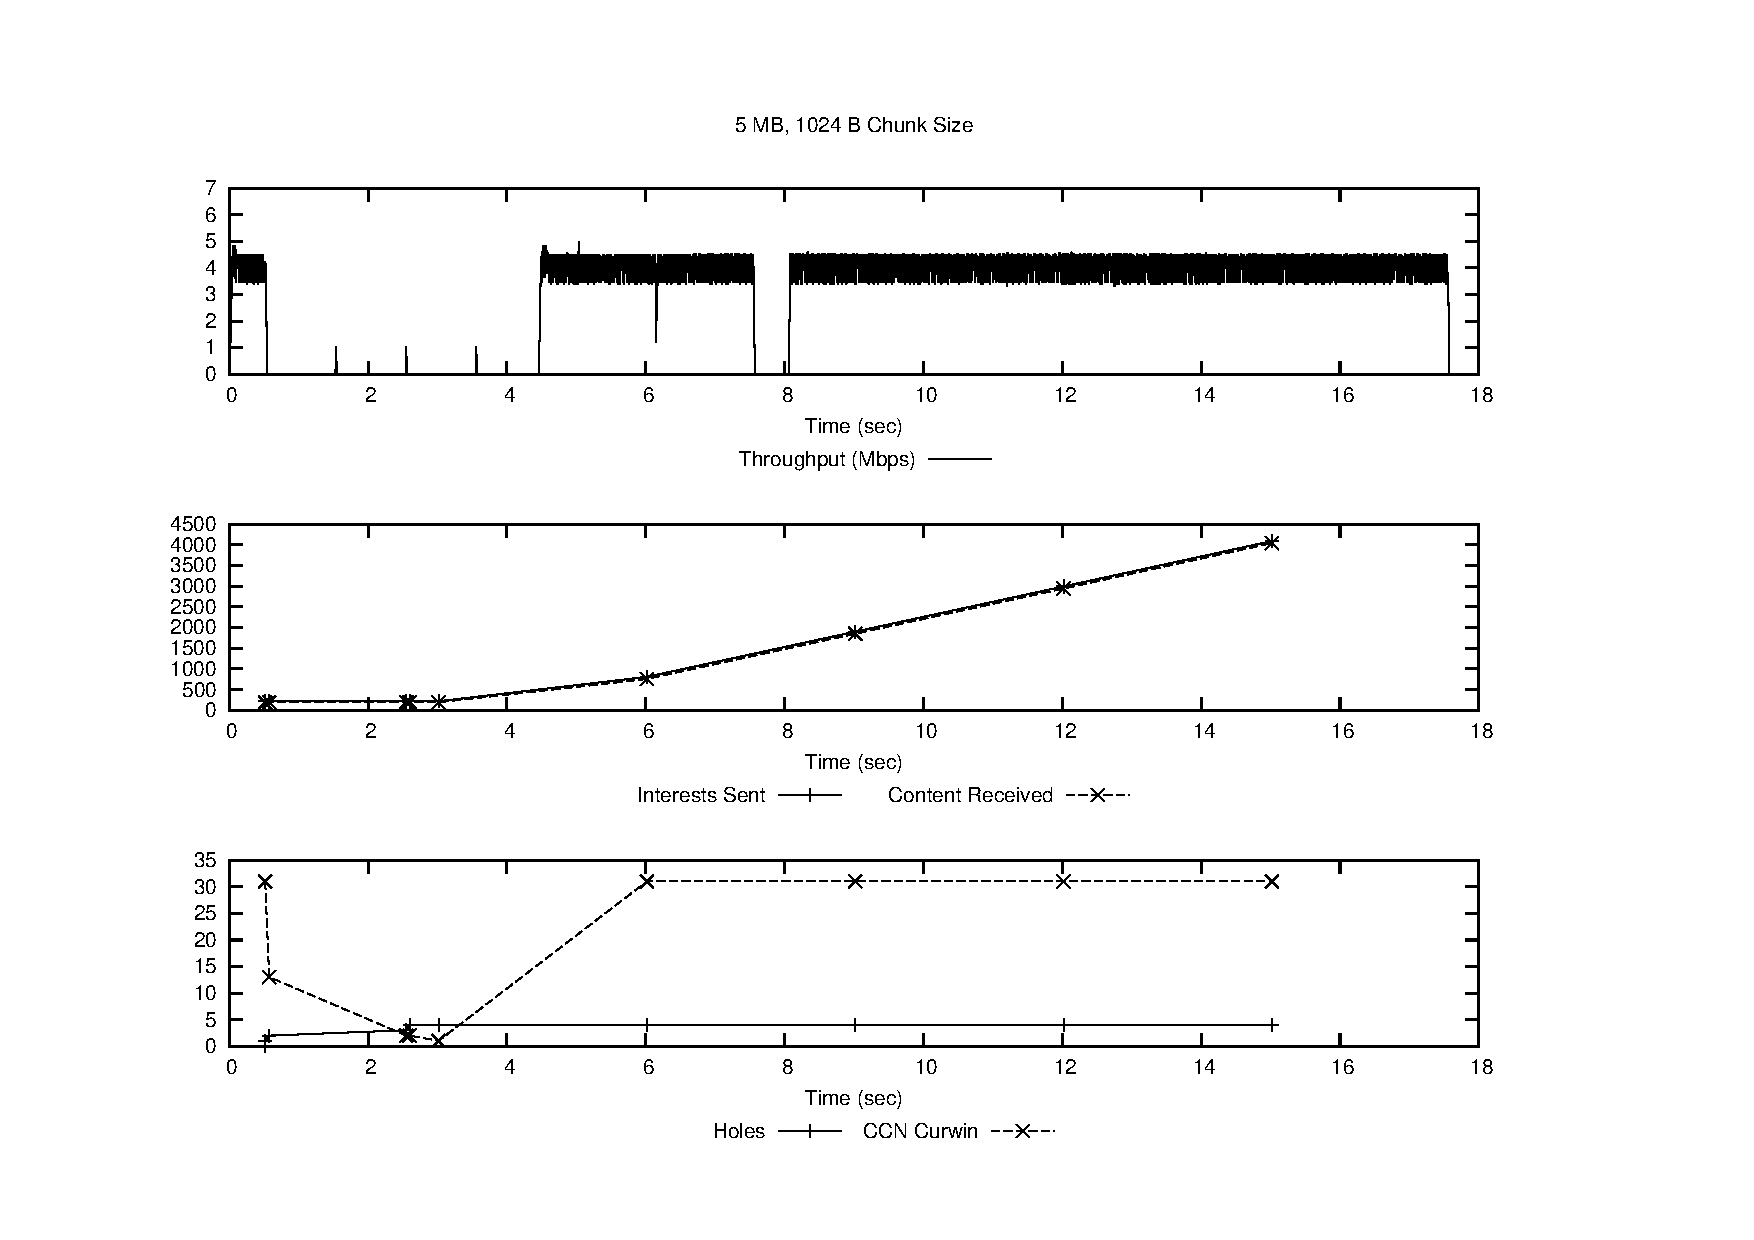
\includegraphics[width=0.75\textwidth]{figures/udp_5_1024.pdf}
    \cprotect\caption{Results for Test 1: Throughput in Mbps, as perceived by 
        PC1, when retrieving a file of size 5\,MB with a 1024 byte 
        `chunk' size. Statistics specific to the \verb+ccncatchunks2+ application 
        are also shown.}
    \label{fig:test-1-thpt-5-1024}

\end{figure}

\begin{figure}[H]

    \centering
    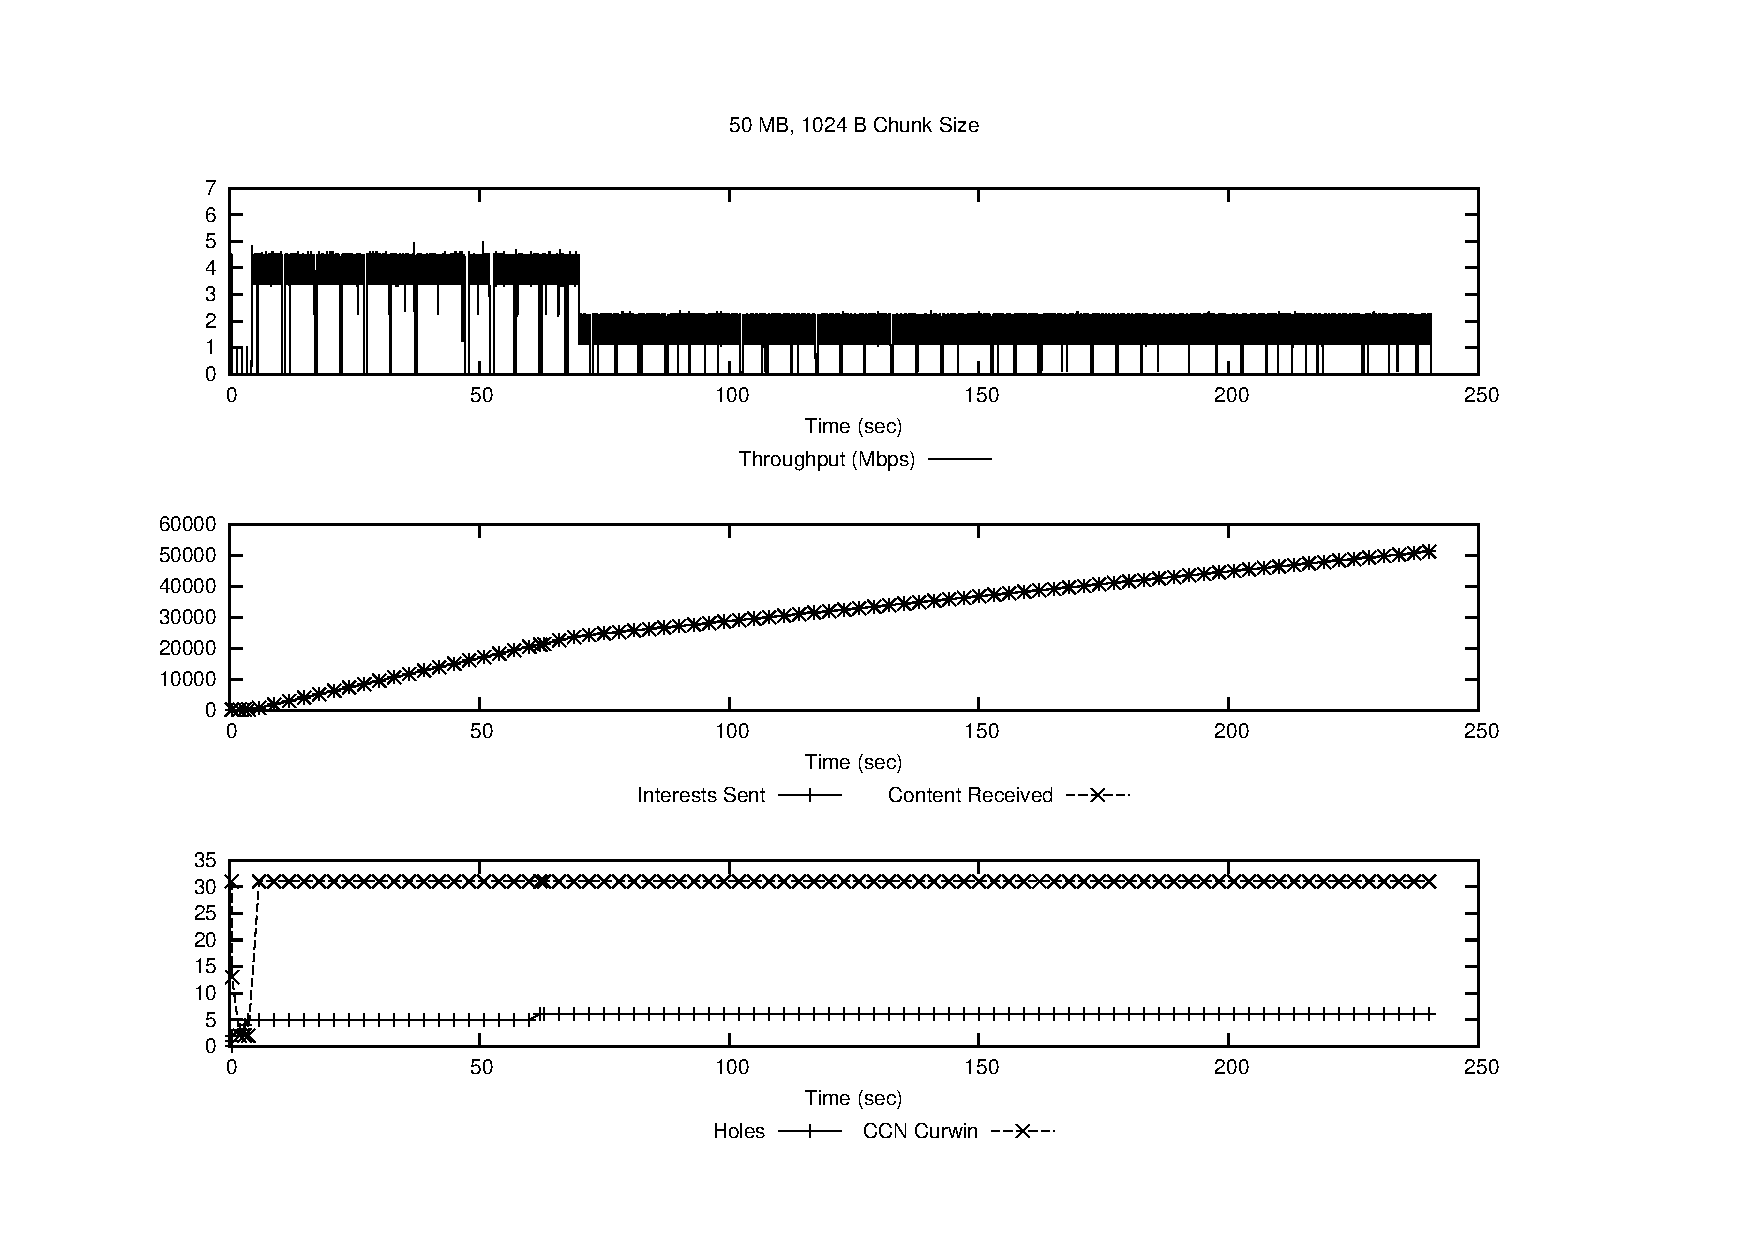
\includegraphics[width=0.75\textwidth]{figures/udp_50_1024.pdf}
    \cprotect\caption{Results for Test 1: Throughput in Mbps, as perceived by 
        PC1, when retrieving a file of size 50\,MB with a 1024 byte 
        `chunk' size. Statistics specific to the \verb+ccncatchunks2+ application 
        are also shown.}
    \label{fig:test-1-thpt-50-1024}

\end{figure}

\begin{figure}[H]

    \centering
    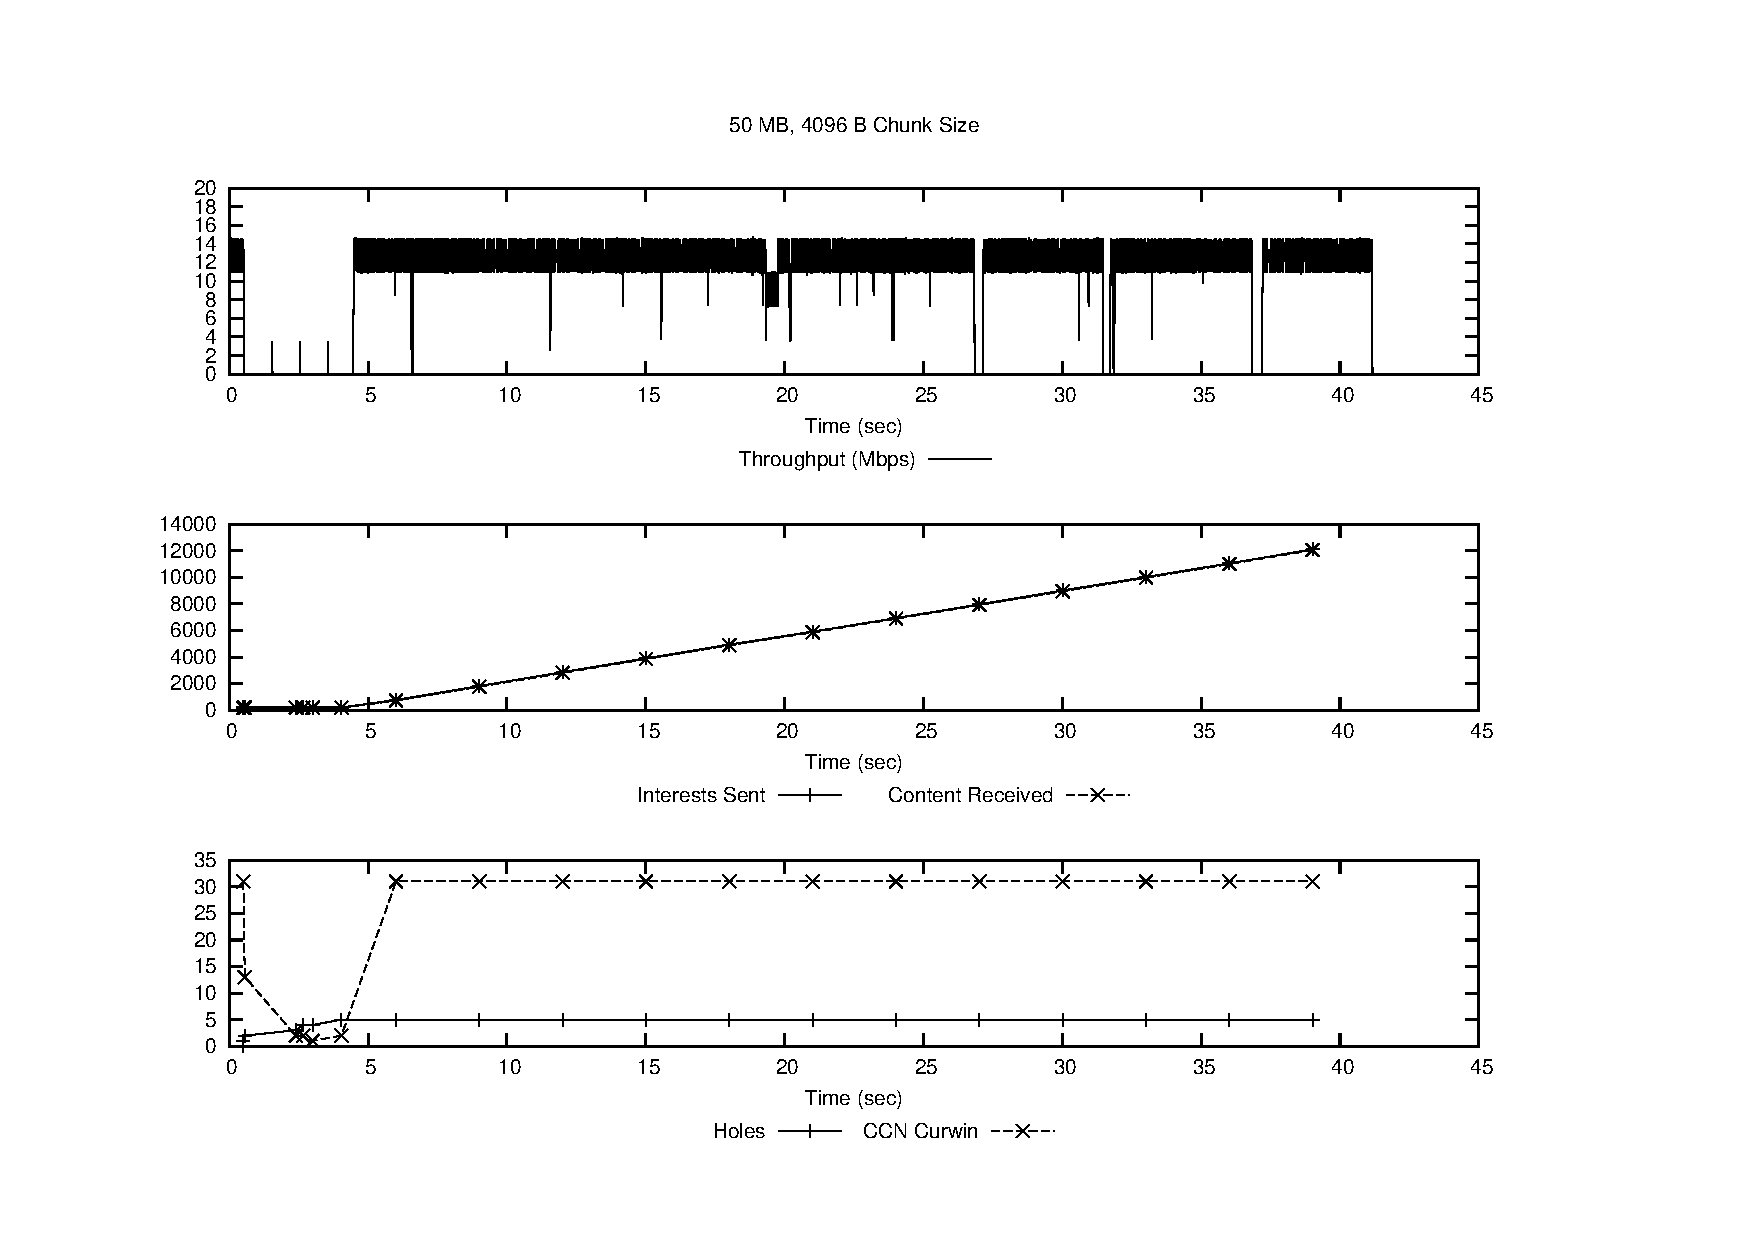
\includegraphics[width=0.75\textwidth]{figures/udp_50_4096.pdf}
    \cprotect\caption{Results for Test 1: Throughput in Mbps, as perceived by 
        PC1, when retrieving a file of size 50\,MB with a 4096 byte 
        `chunk' size. Statistics specific to the \verb+ccncatchunks2+ application 
        are also shown.}
    \label{fig:test-1-thpt-50-4096}

\end{figure}

\begin{figure}[H]

    \centering
    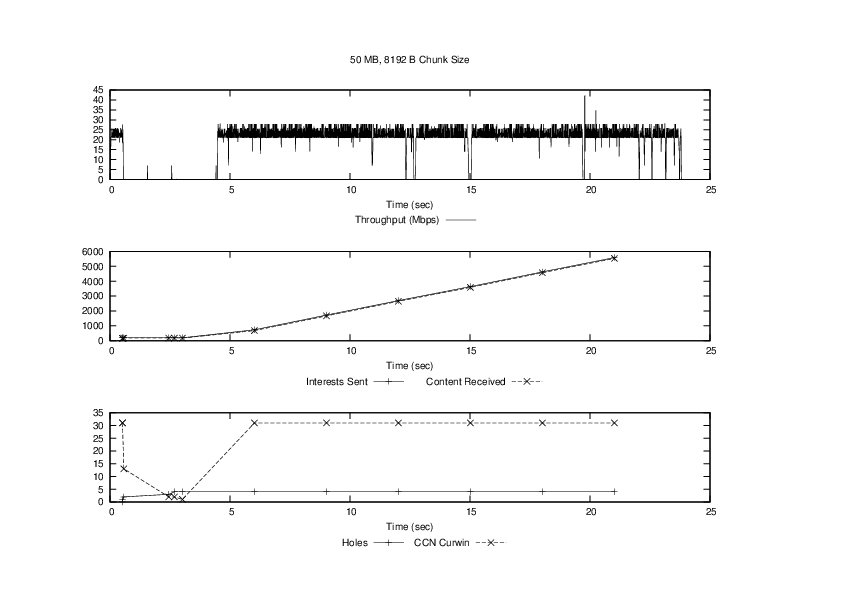
\includegraphics[width=0.75\textwidth]{figures/udp_50_8192.pdf}
    \cprotect\caption{Results for Test 1: Throughput in Mbps, as perceived by 
        PC1, when retrieving a file of size 50\,MB with a 8192 byte 
        `chunk' size. Statistics specific to the \verb+ccncatchunks2+ application 
        are also shown.}
    \label{fig:test-1-thpt-50-8192}

\end{figure}

\begin{figure}[H]

    \centering
    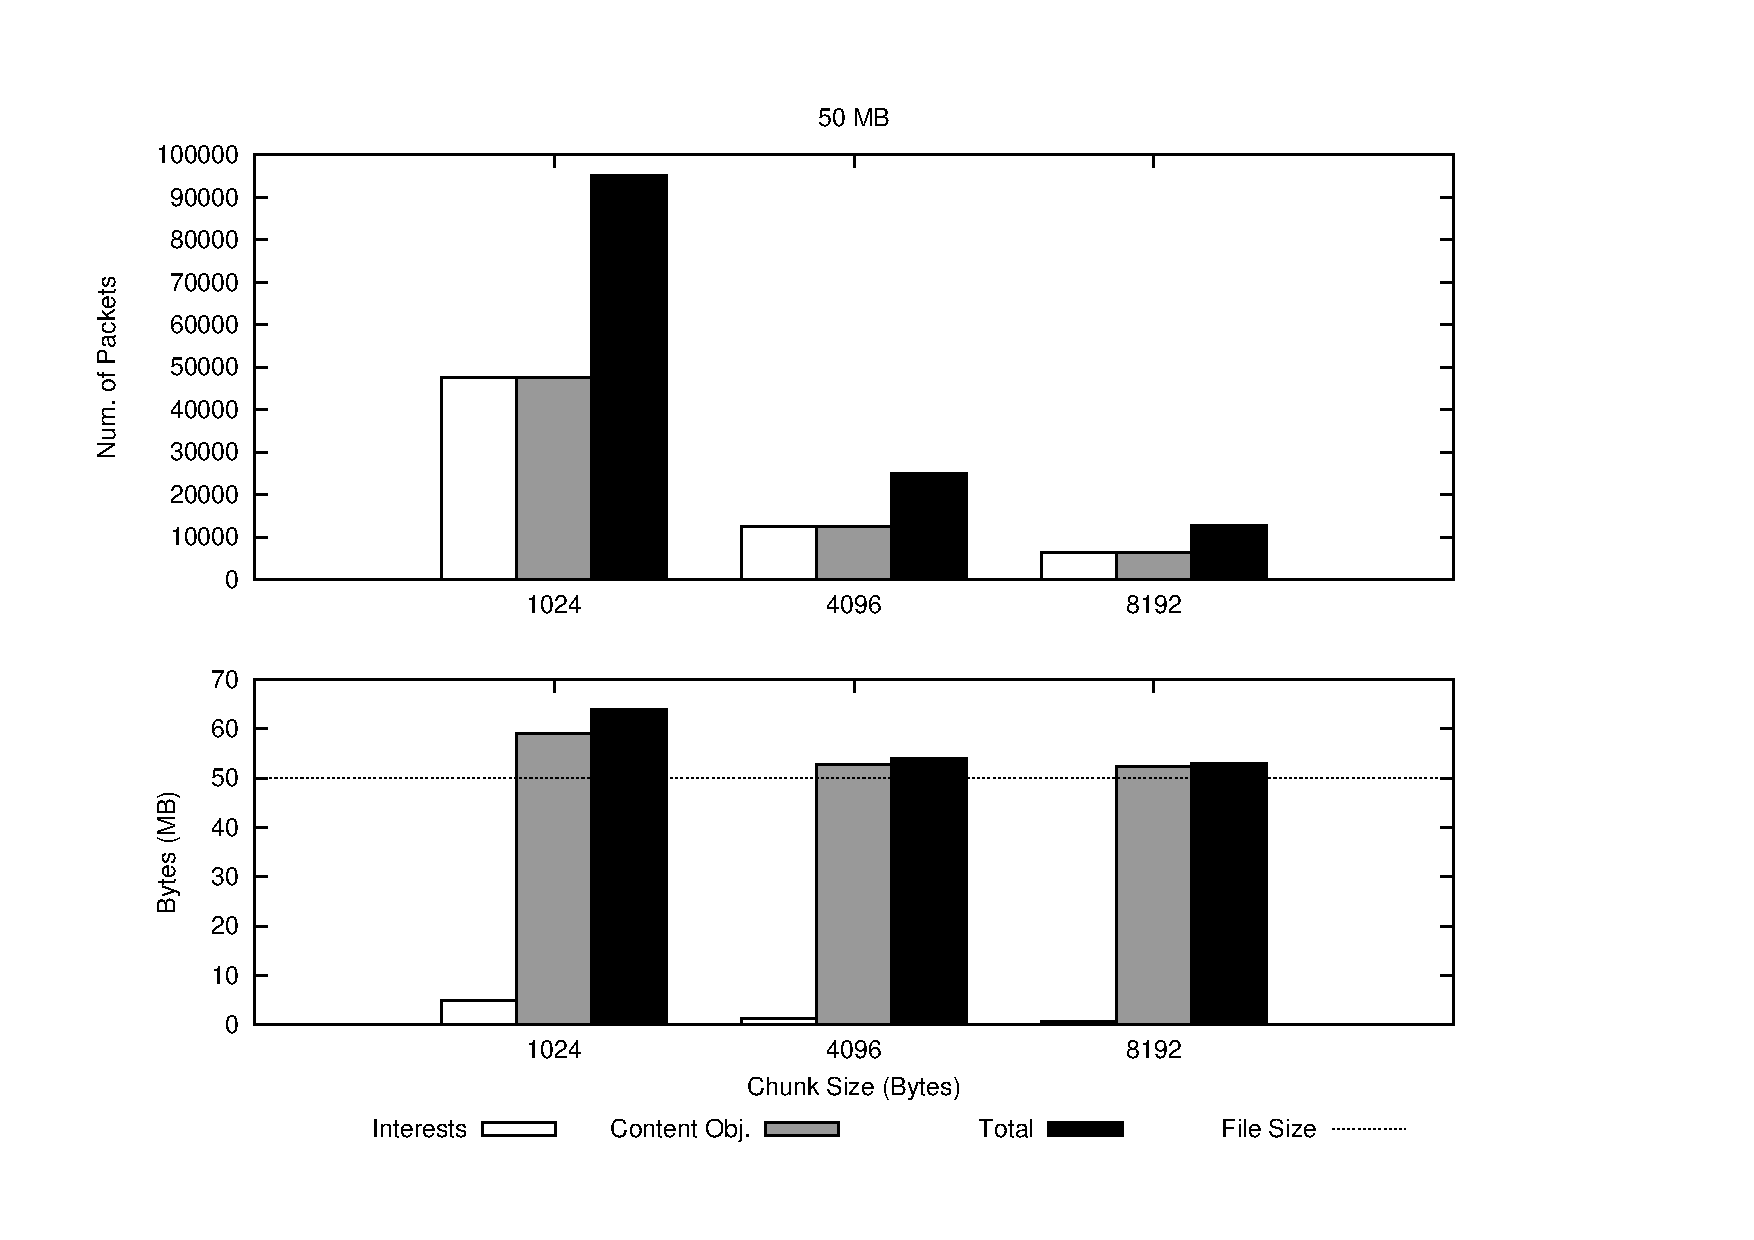
\includegraphics[width=0.75\textwidth]{figures/udp_50.pdf}
    \cprotect\caption{Results for Test 1: Packet and byte quantities, measured 
        at PC1, for a file size of 50\,MB.}
    \label{fig:test-1-packets-bytes-50}

\end{figure}

\begin{figure}[H]

    \centering
    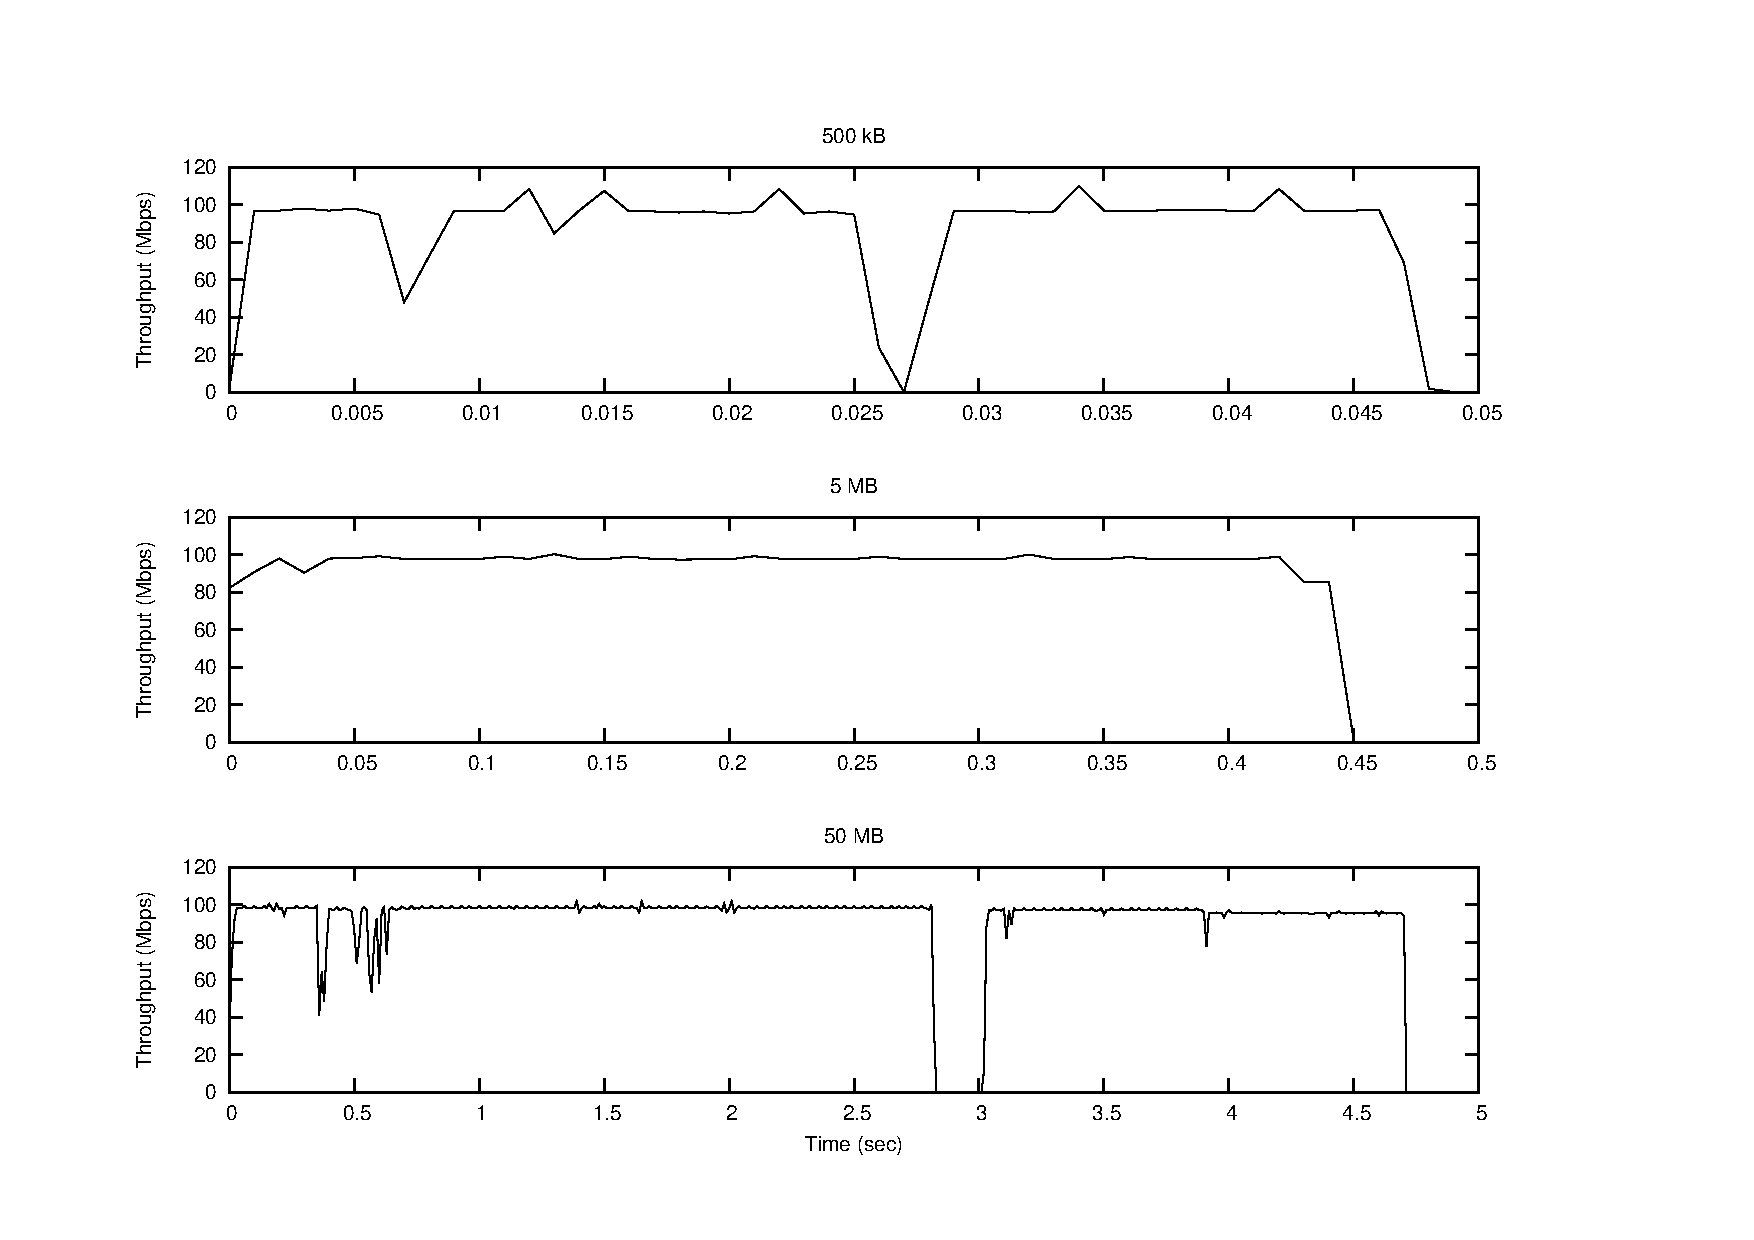
\includegraphics[width=0.75\textwidth]{figures/ftp-thpt.pdf}
    \cprotect\caption{Results for Test 1: Throughput in Mbps, as perceived by 
        PC1, when retrieving files of sizes 500\,kB, 5\,MB and 50\,MB, over 
        FTP.}
    \label{fig:test-1-thpt-ftp}

\end{figure}

\begin{figure}[H]

    \centering
    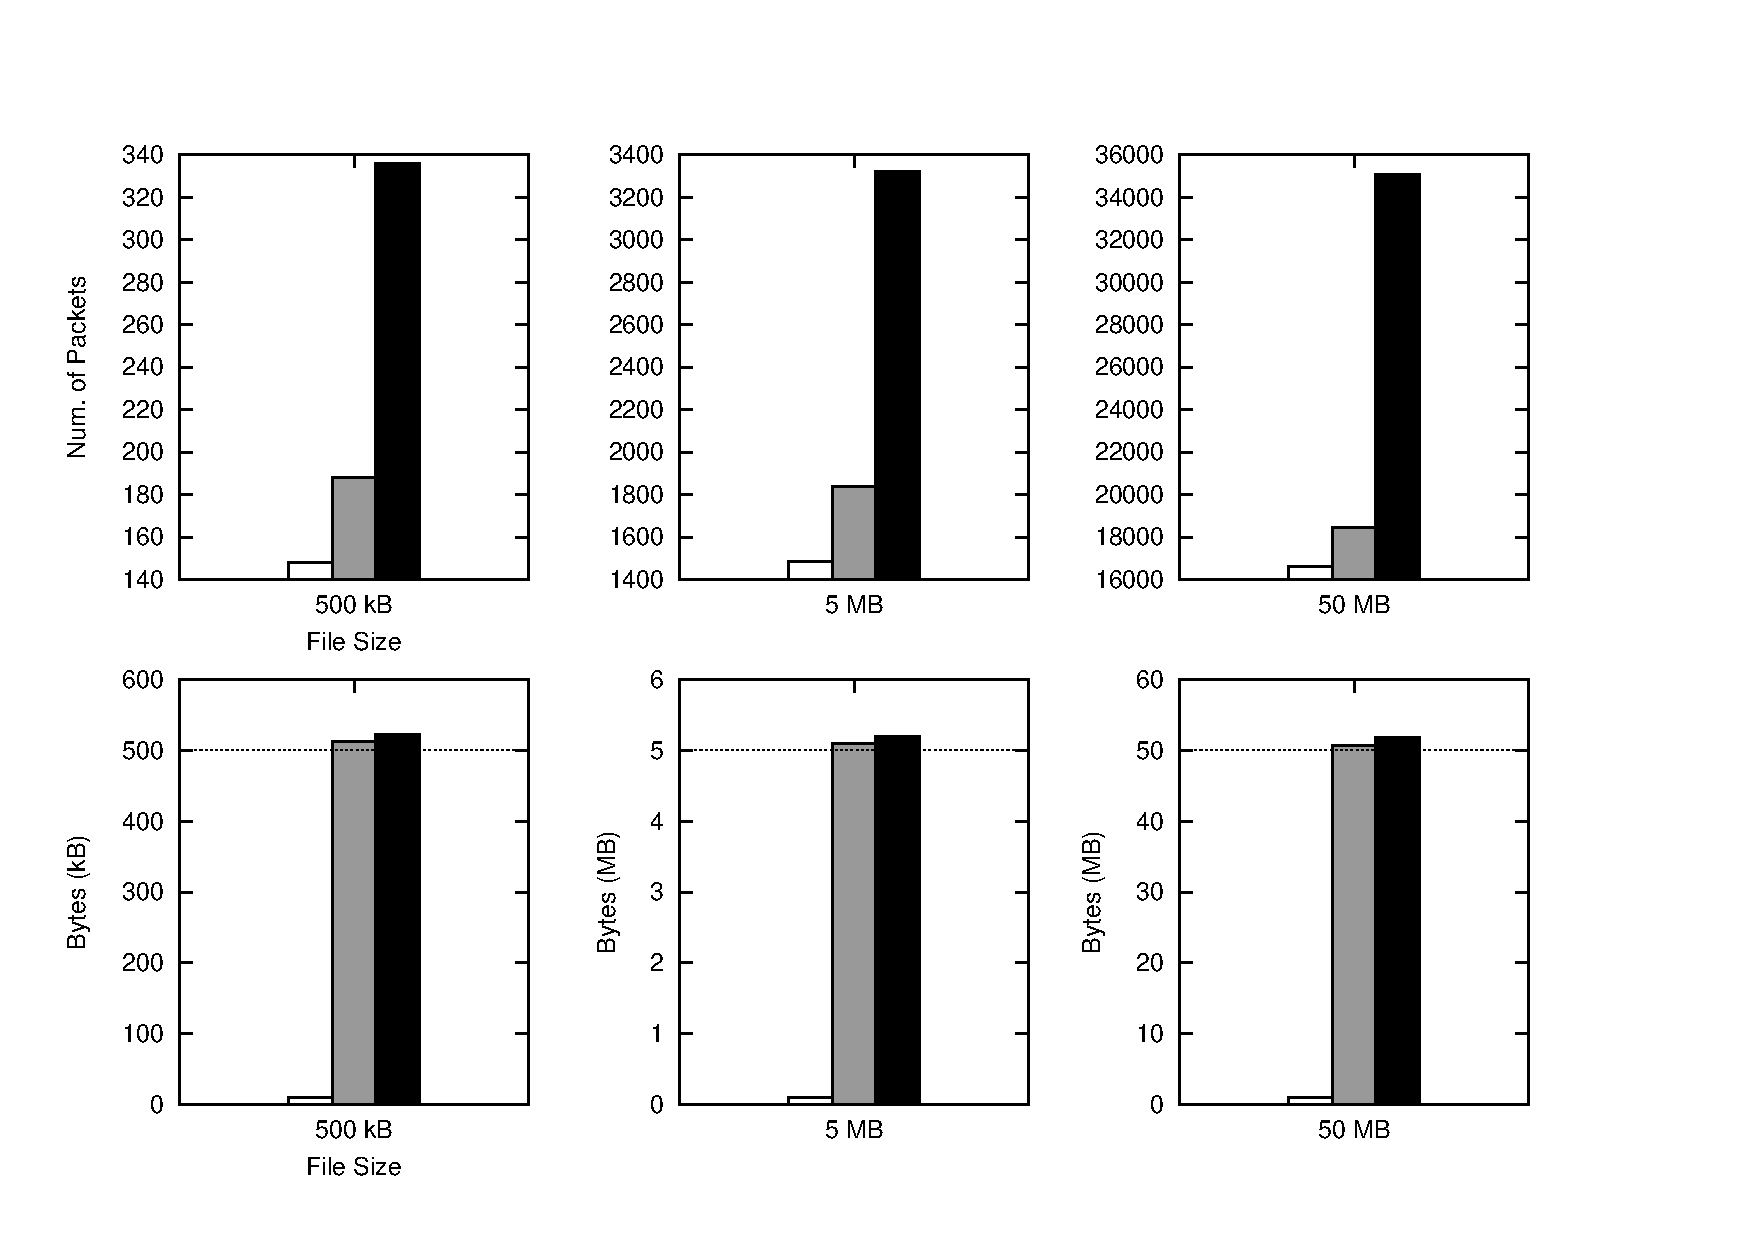
\includegraphics[width=0.75\textwidth]{figures/tcp.pdf}
    \cprotect\caption{Results for Test 1: Packet and byte quantities, measured 
        at PC1, for files of sizes 500\,kB, 5\,MB and 50\,MB, over 
        FTP. The white bars represent packets sent from the FTP client side, 
        gray represent packets sent from the FTP server side, while the 
        black bars represent the total number of exchanged packets.}
    \label{fig:test-1-packets-bytes-ftp}

\end{figure}

\section{Test 2 - CCNx Multihop Forwarding}
\label{app:res-multihop-for}

\subsection{Test 2.1 - CCNx Multihop Forwarding (File Transfer)}
\label{subapp:test-multihop-file}

\begin{figure}[H]
    \centering

    \subfigure[]{
        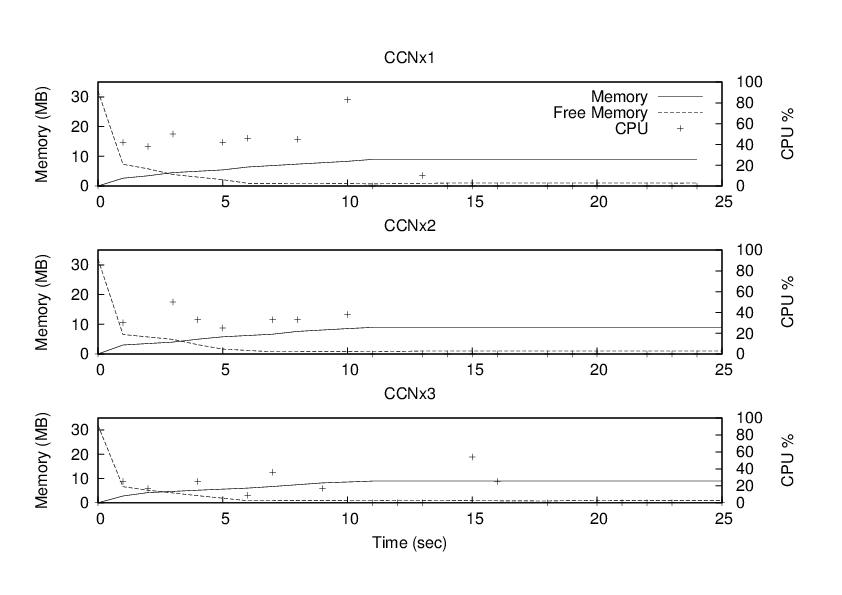
\includegraphics[width=0.75\textwidth] {figures/file_5-sep-cpu-mem.pdf}
        \label{subfig:file_5-sep-cpu-mem}
    }

    \subfigure[]{
        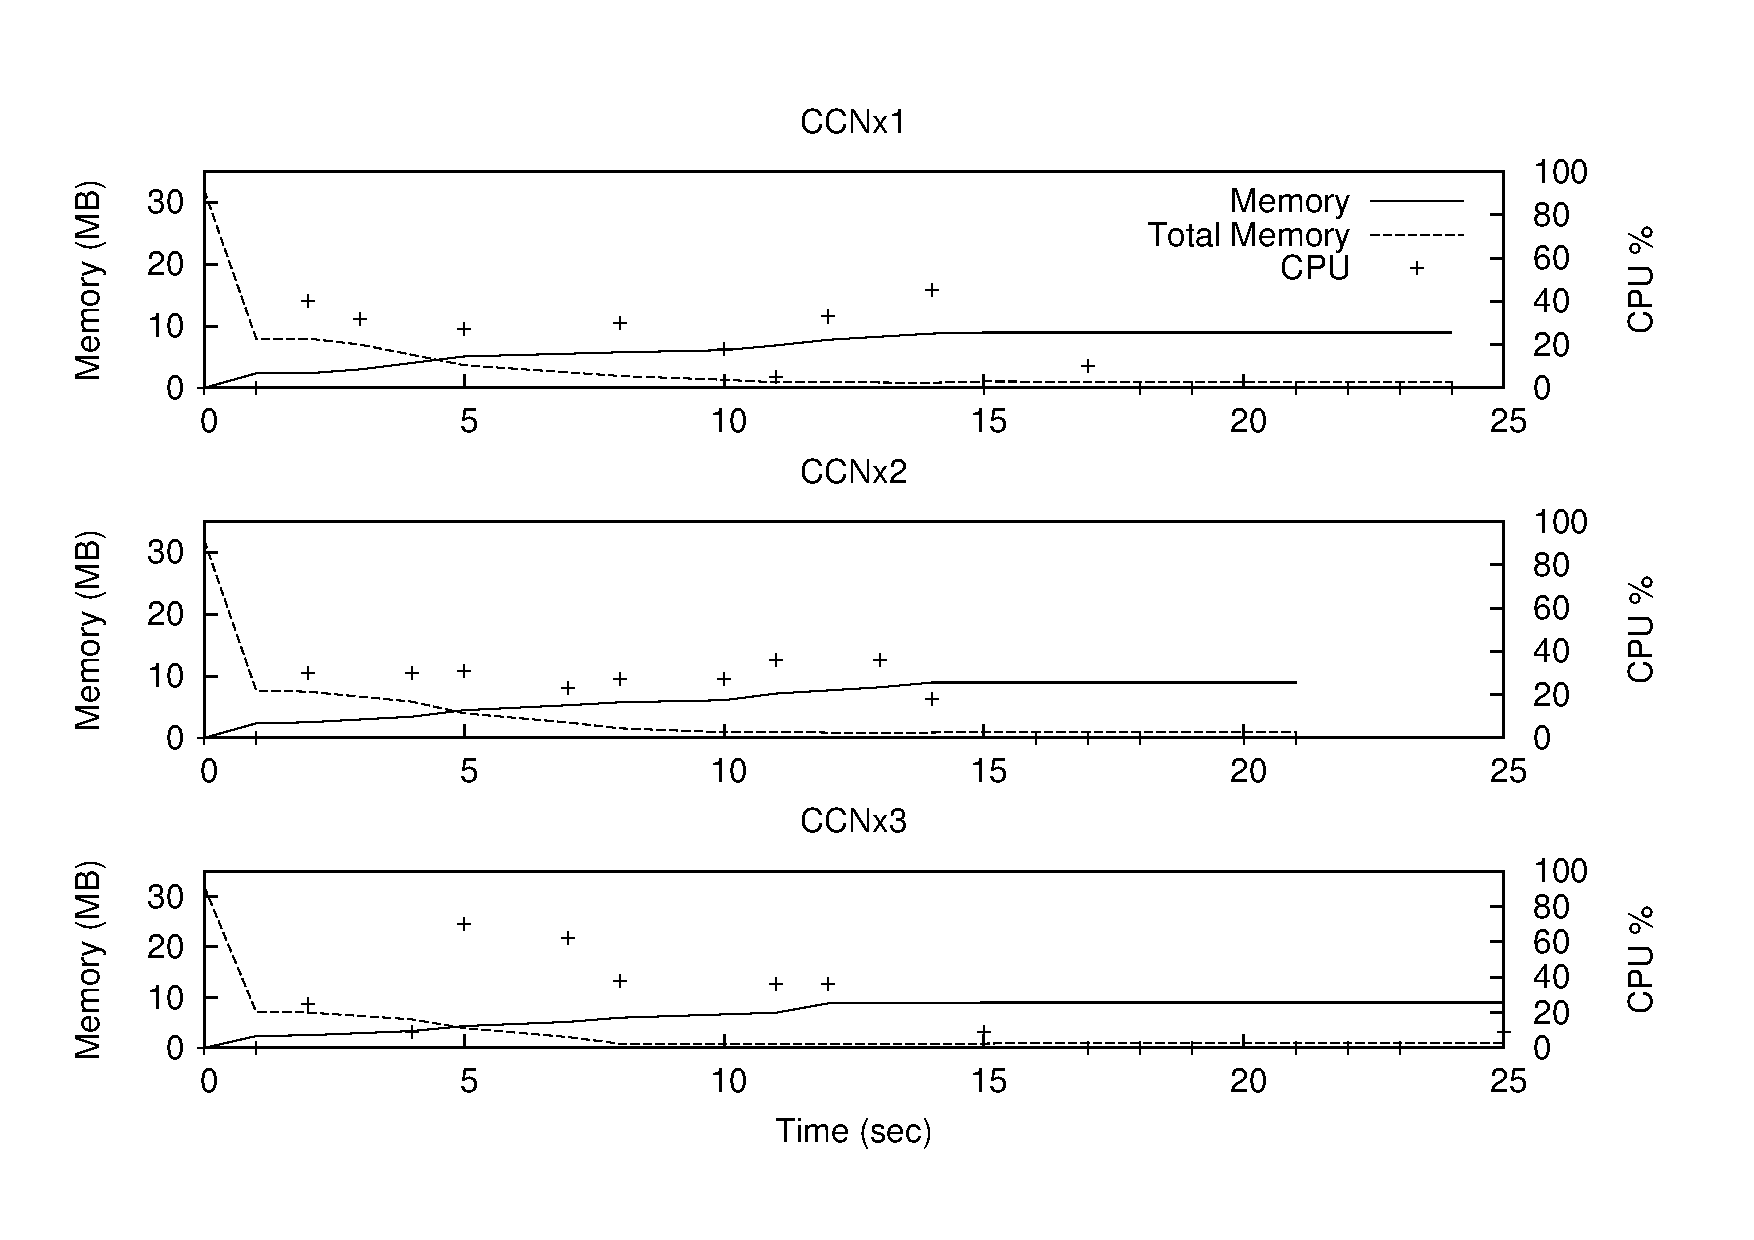
\includegraphics[width=0.75\textwidth] {figures/file_5-sim-cpu-mem.pdf}
        \label{subfig:file_5-sim-cpu-mem}
    }

    \cprotect\caption{Results for Test 2.1: CPU and memory utilization at 
        all CCNx nodes, during the transfer of a file of size 
        5\,MB, for both non-overlapping (a) and overlapping (b) cases. Regarding the 
        memory values, the `memory' line corresponds to the amount of RAM 
        occupied by the \verb+ccnd+ process, while the `free memory' corresponds 
        to the amount of free memory in the system.}
    \label{fig:file_5-cpu-mem}

\end{figure}

\begin{figure}[H]
    \centering

    \subfigure[]{
        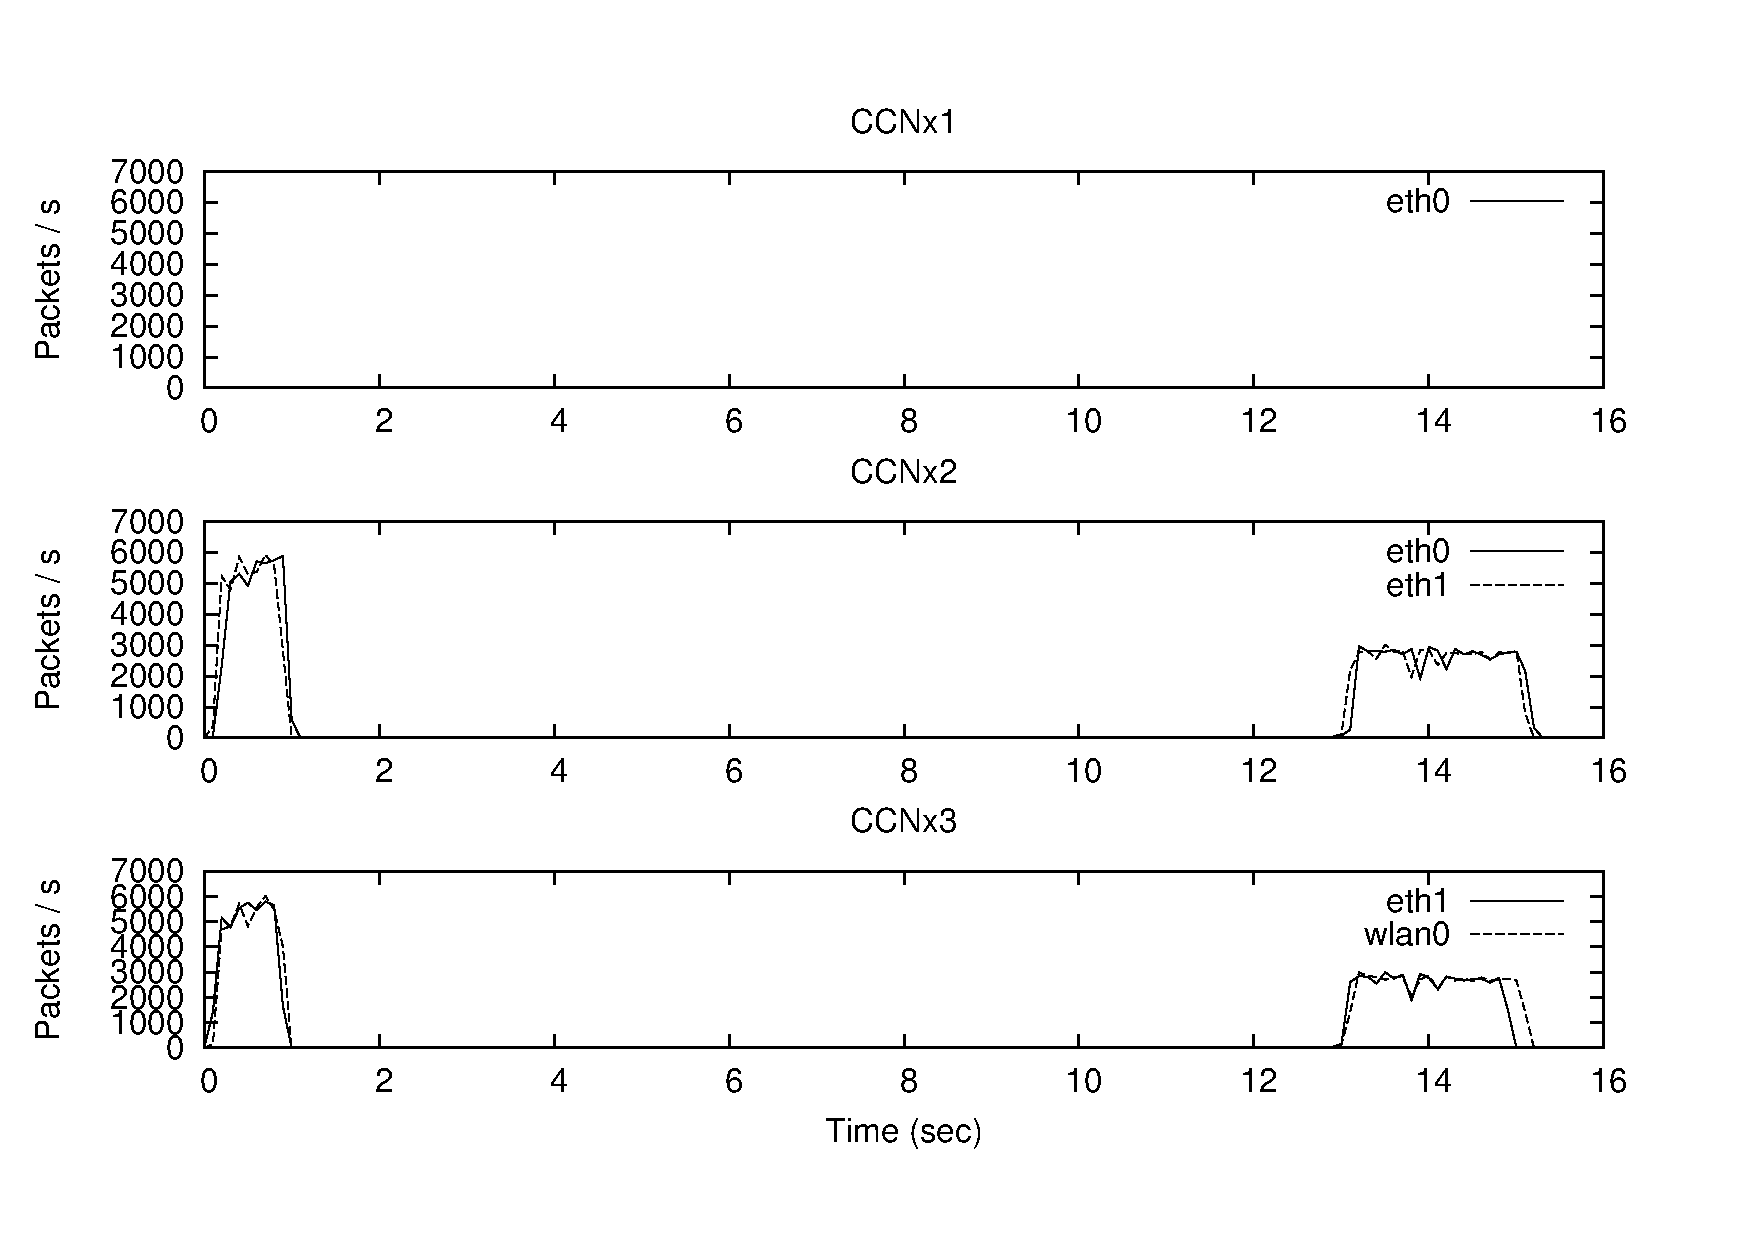
\includegraphics[width=0.75\textwidth] {figures/file_5-ctrl-net.pdf}
        \label{subfig:file_5-ctrl-net}
    }

    \subfigure[]{
        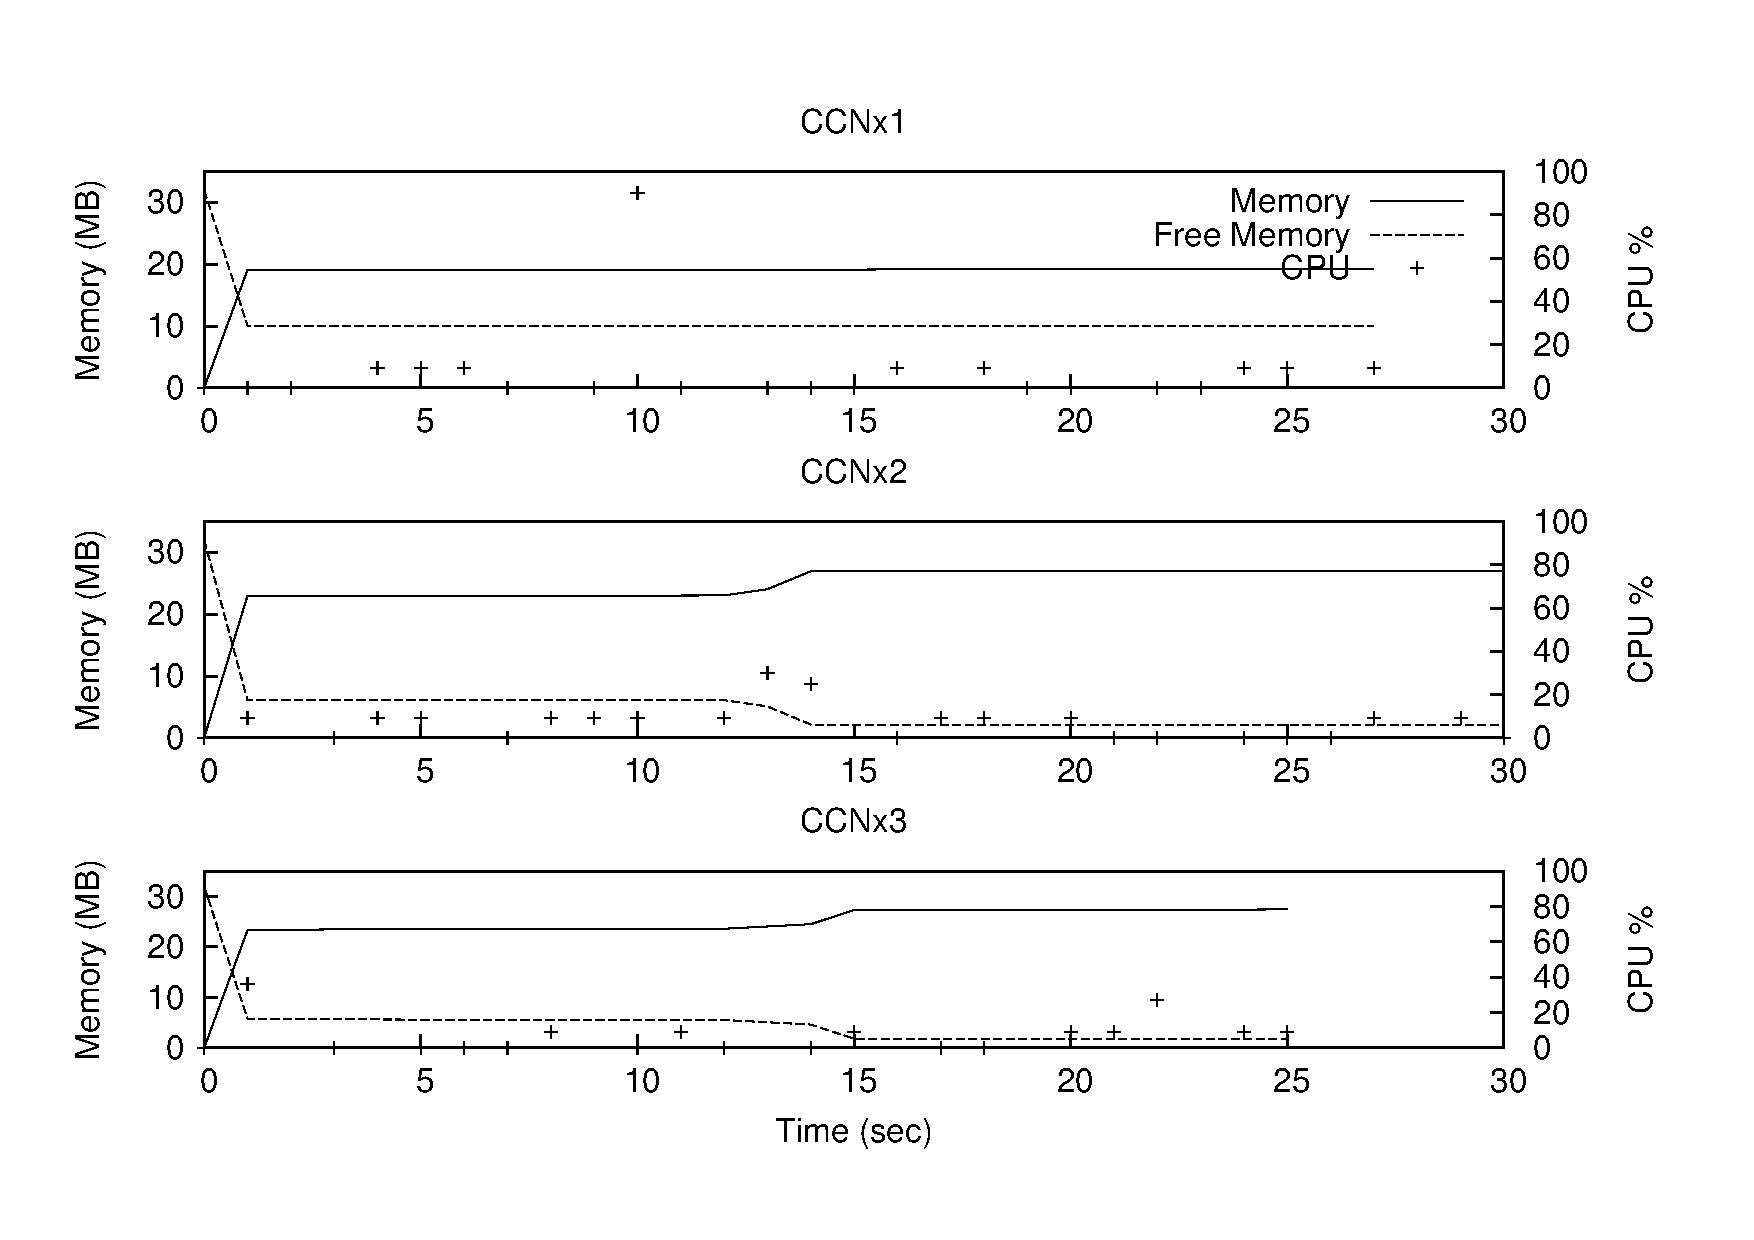
\includegraphics[width=0.75\textwidth] {figures/file_5-ctrl-cpu-mem.pdf}
        \label{subfig:file_5-ctrl-cpu-mem}
    }

    \cprotect\caption{Results for Test 2.1: Network load (a) and 
        CPU and memory utilization (b) at 
        all routing nodes, during the transfer of a file of size 
        5\,MB over FTP, for a non-overlapping case. Regarding the 
        memory values, the `memory' line corresponds to the amount of RAM 
        occupied by the \verb+ccnd+ process, while the `free memory' corresponds 
        to the amount of free memory in the system.}
    \label{fig:file_5-ctrl}

\end{figure}

\subsection{Test 2.2 - CCNx Multihop Forwarding (Video Streaming)}
\label{subapp:test-multihop-video}

\begin{figure}[H]
    \centering

    \subfigure[]{
        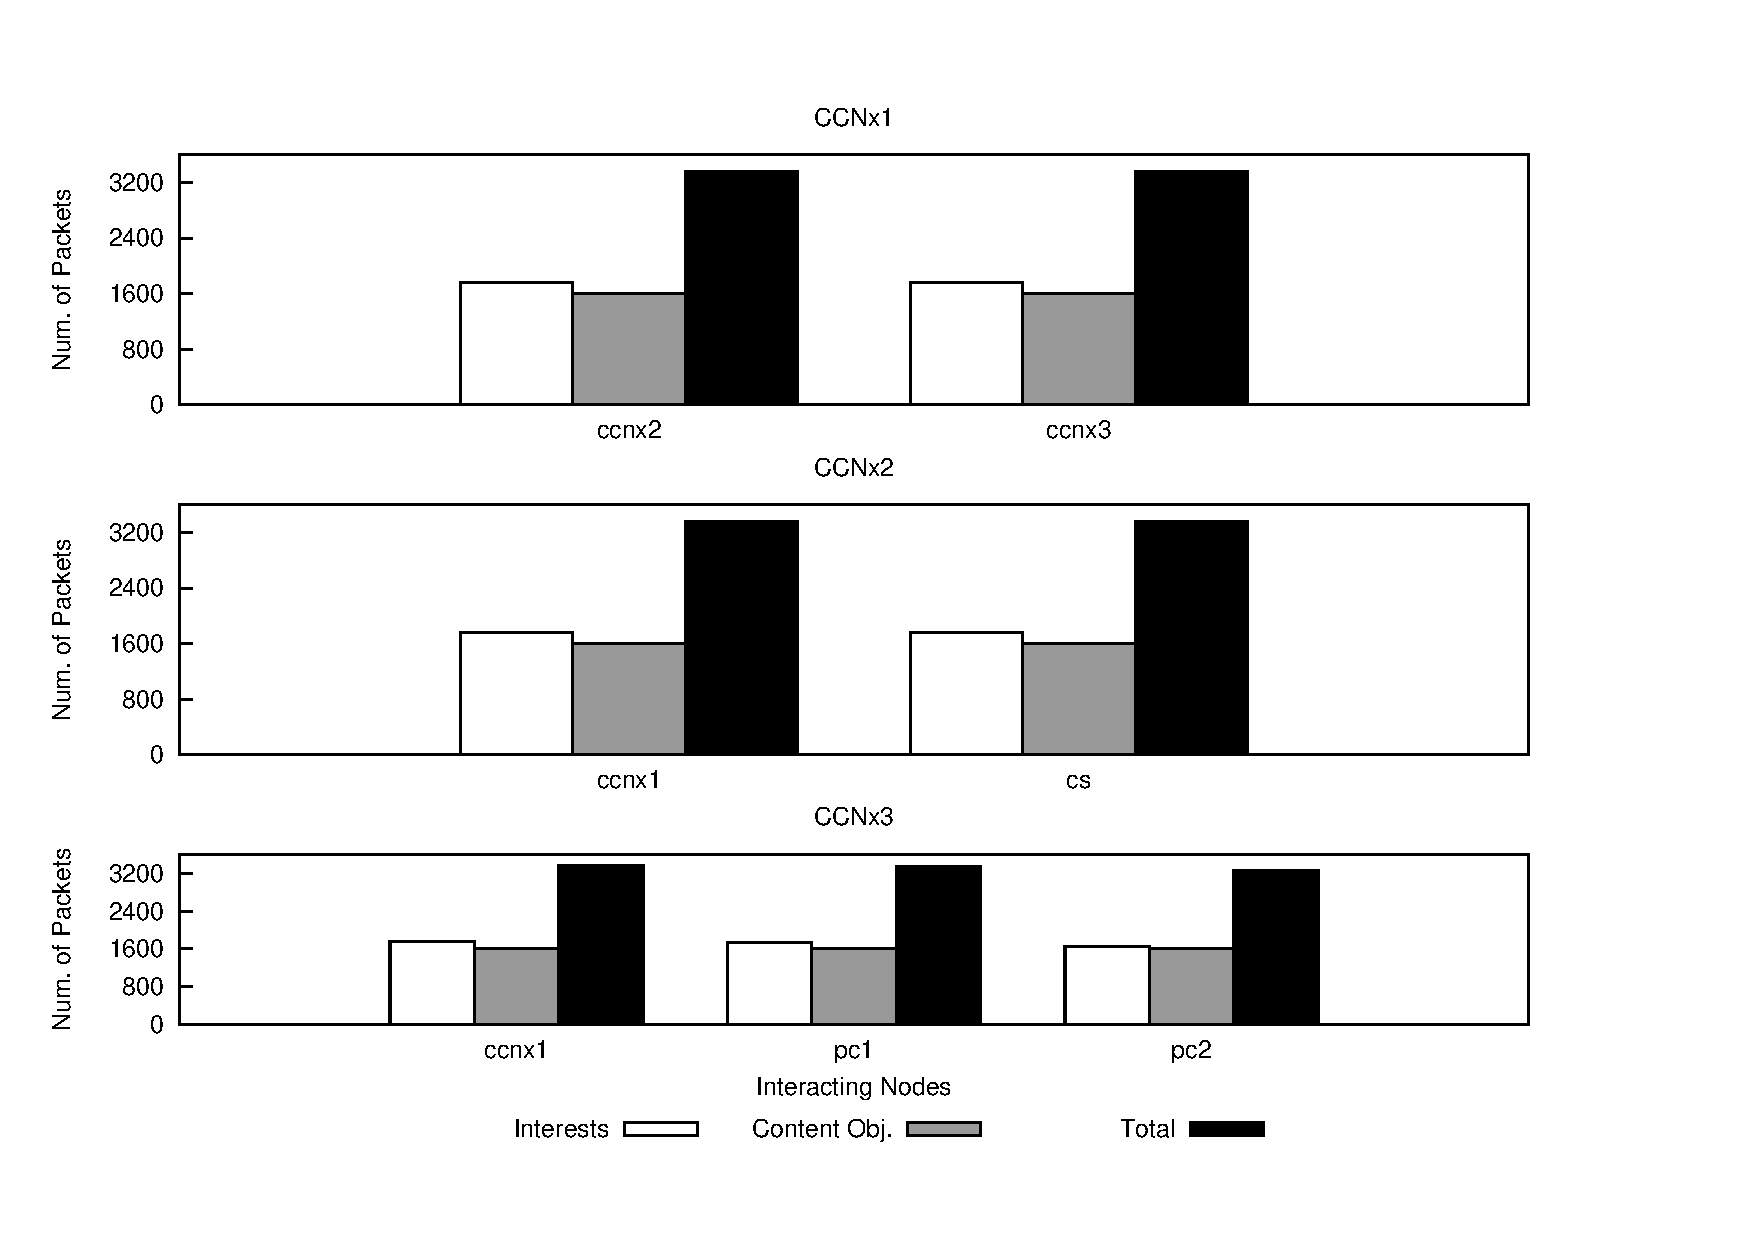
\includegraphics[width=0.75\textwidth] {figures/video-sep-pckt.pdf}
        \label{subfig:video-sep-pckt}
    }

    \subfigure[]{
        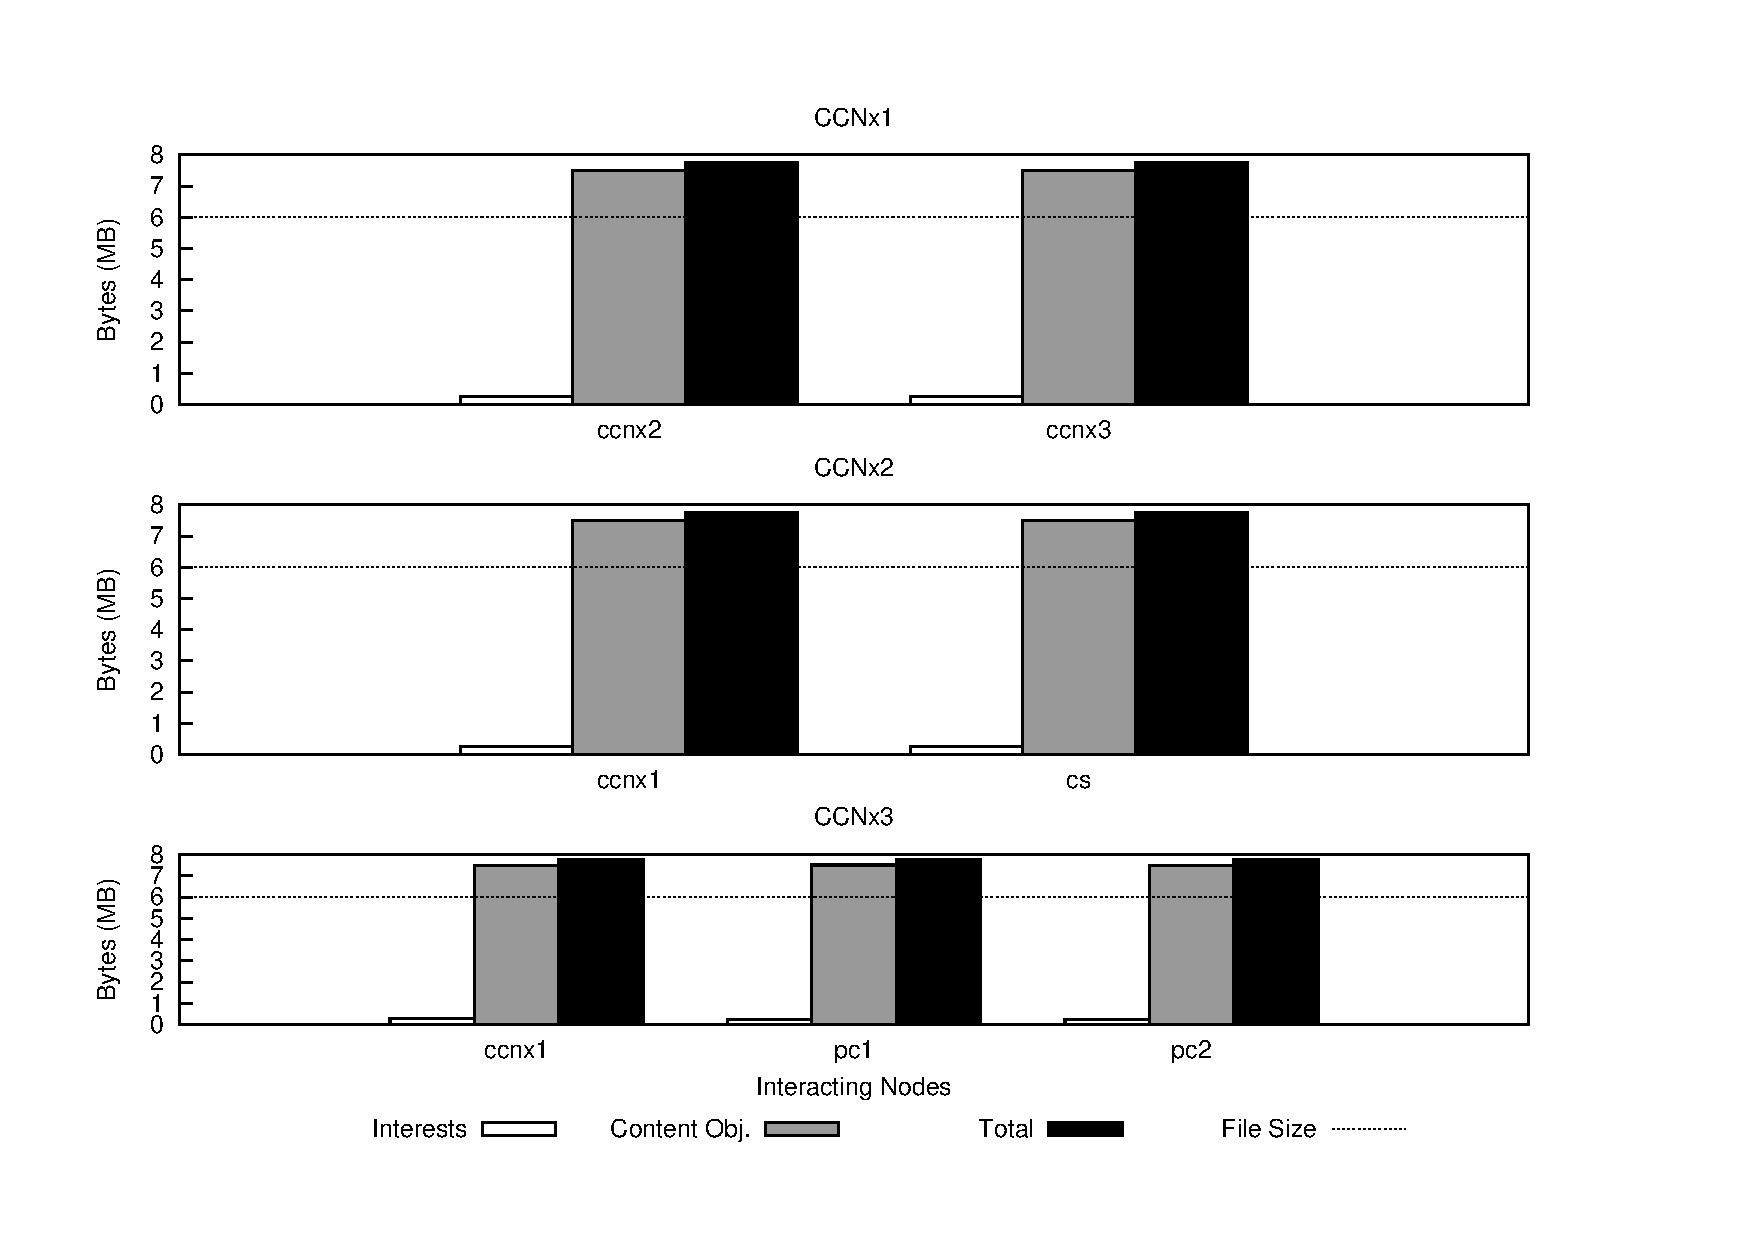
\includegraphics[width=0.75\textwidth] {figures/video-sep-byte.pdf}
        \label{subfig:video-sep-byte}
    }

    \cprotect\caption{Results for Test 2.2: Packet (a) and byte (b) 
        counts (Interest and 
        Content Objects) registered at each CCNx forwarding node, exchanged 
        between the respective peer elements. This test involves the 
        streaming of a video of size 6.3\,MB and 8 seconds duration from 
        the content source CS to nodes PC1 and PC2 (see Figure~\ref{fig:basic-testbed}).}
    \label{fig:video-sep-abs}

\end{figure}

\begin{figure}[H]
    \centering

    \subfigure[]{
        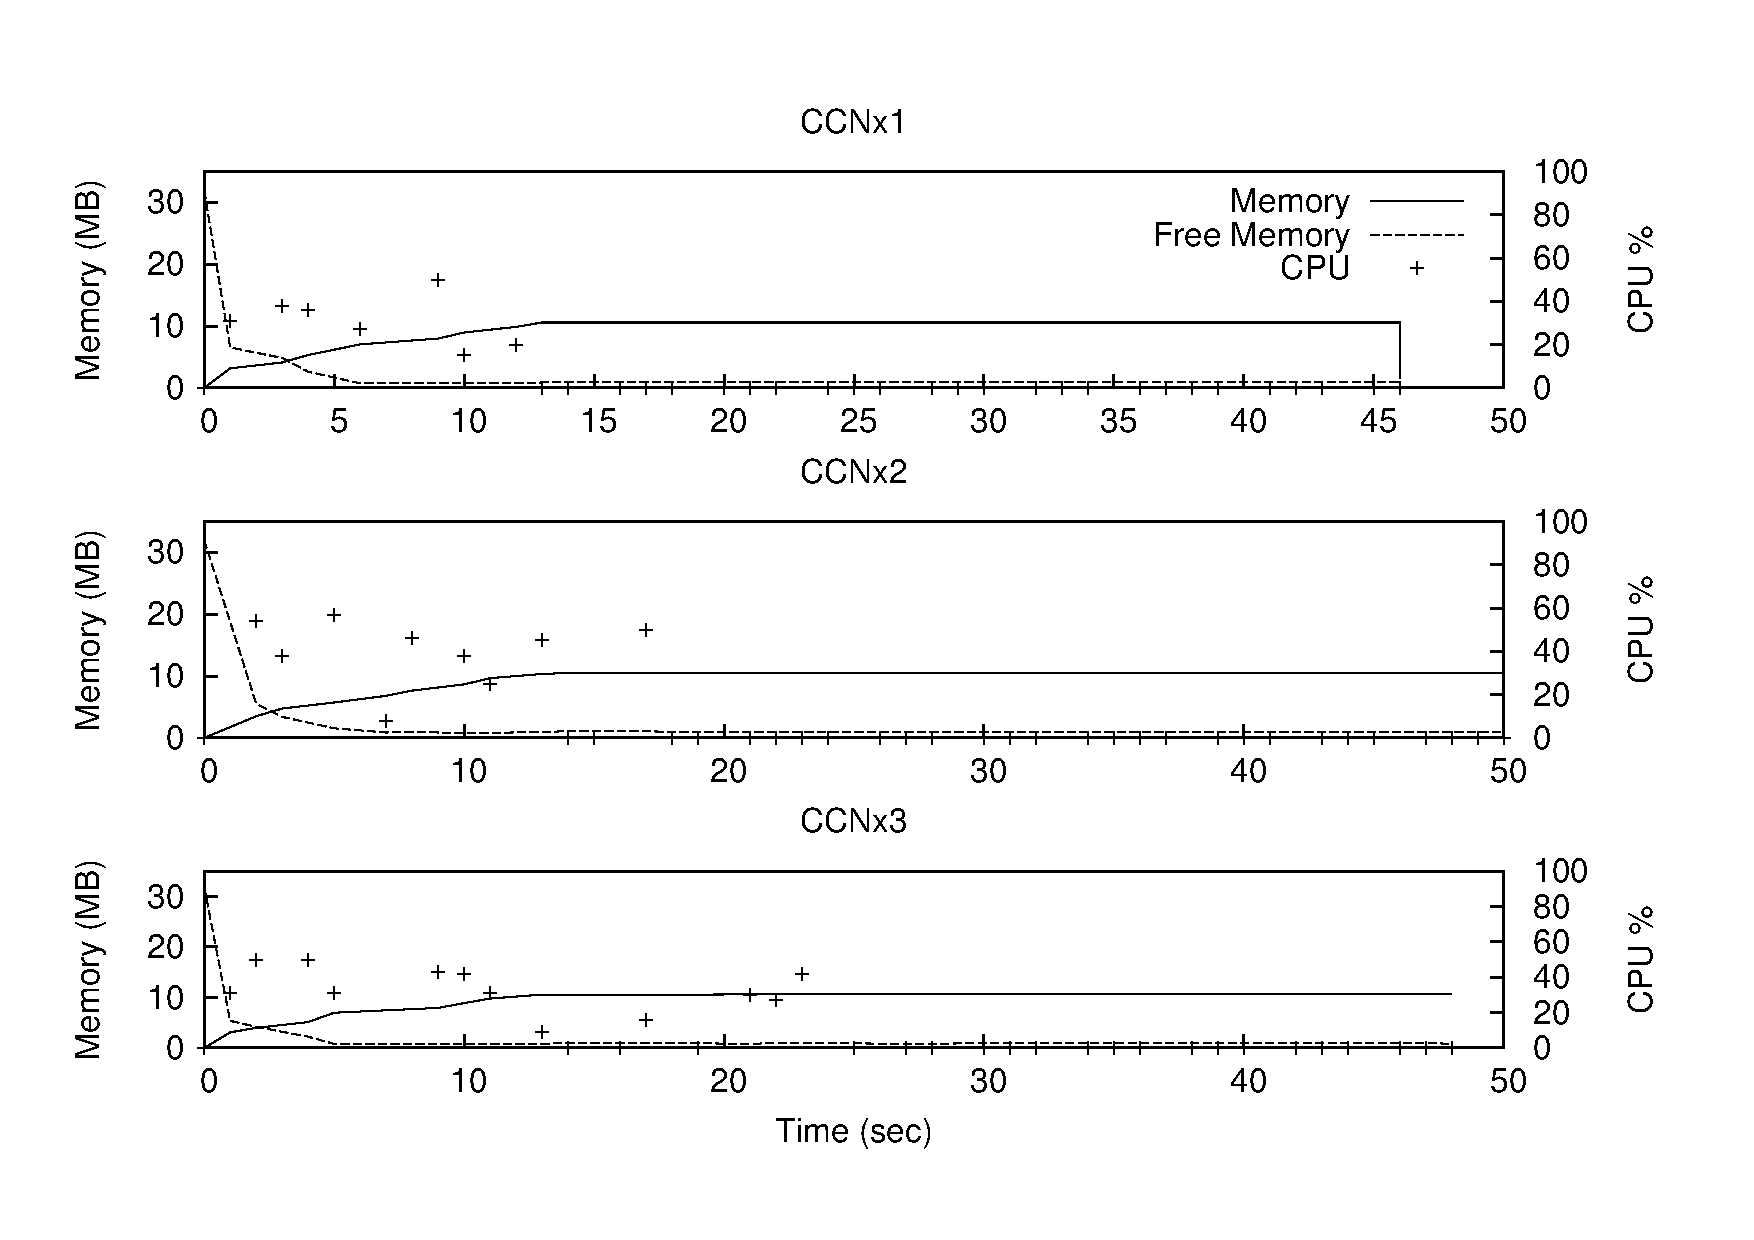
\includegraphics[width=0.75\textwidth] {figures/video-sep-cpu-mem.pdf}
        \label{subfig:video-sep-cpu-mem}
    }

    \subfigure[]{
        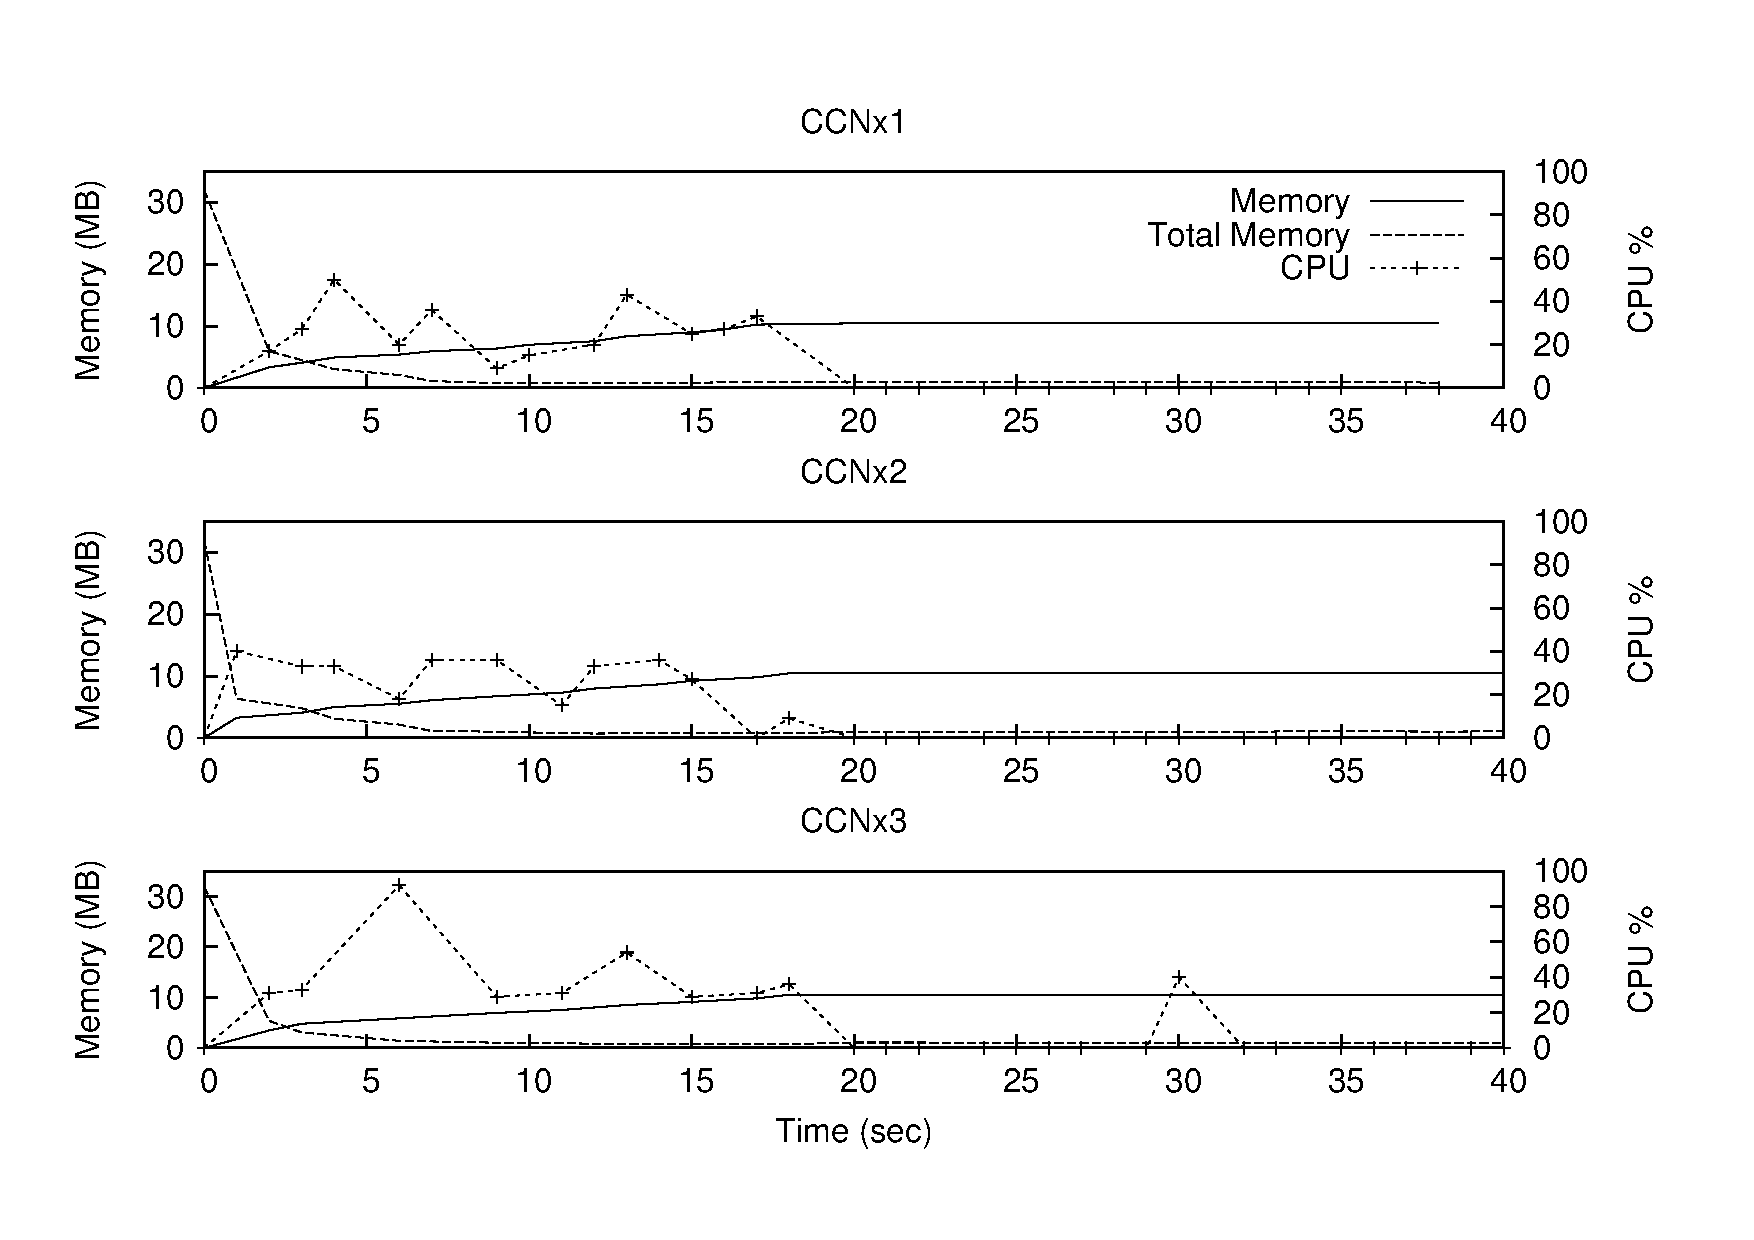
\includegraphics[width=0.75\textwidth] {figures/video-sim-cpu-mem.pdf}
        \label{subfig:video-sim-cpu-mem}
    }

    \cprotect\caption{Results for Test 2.2: CPU and memory utilization at 
        all CCNx nodes, during the streaming of a video file of size 
        6.3\,MB and 8 second duration, for both non-overlapping (a) and 
        overlapping (b) cases. Regarding the 
        memory values, the `memory' line corresponds to the amount of RAM 
        occupied by the \verb+ccnd+ process, while the `free memory' corresponds 
        to the amount of free memory in the system.}
    \label{fig:video-cpu}

\end{figure}

\subsection{Test 2.3 - CCNx Multihop Forwarding (Multiple Paths)}
\label{subapp:test-multihop-multipath}

\begin{figure}[H]
    \centering

    \subfigure[]{
        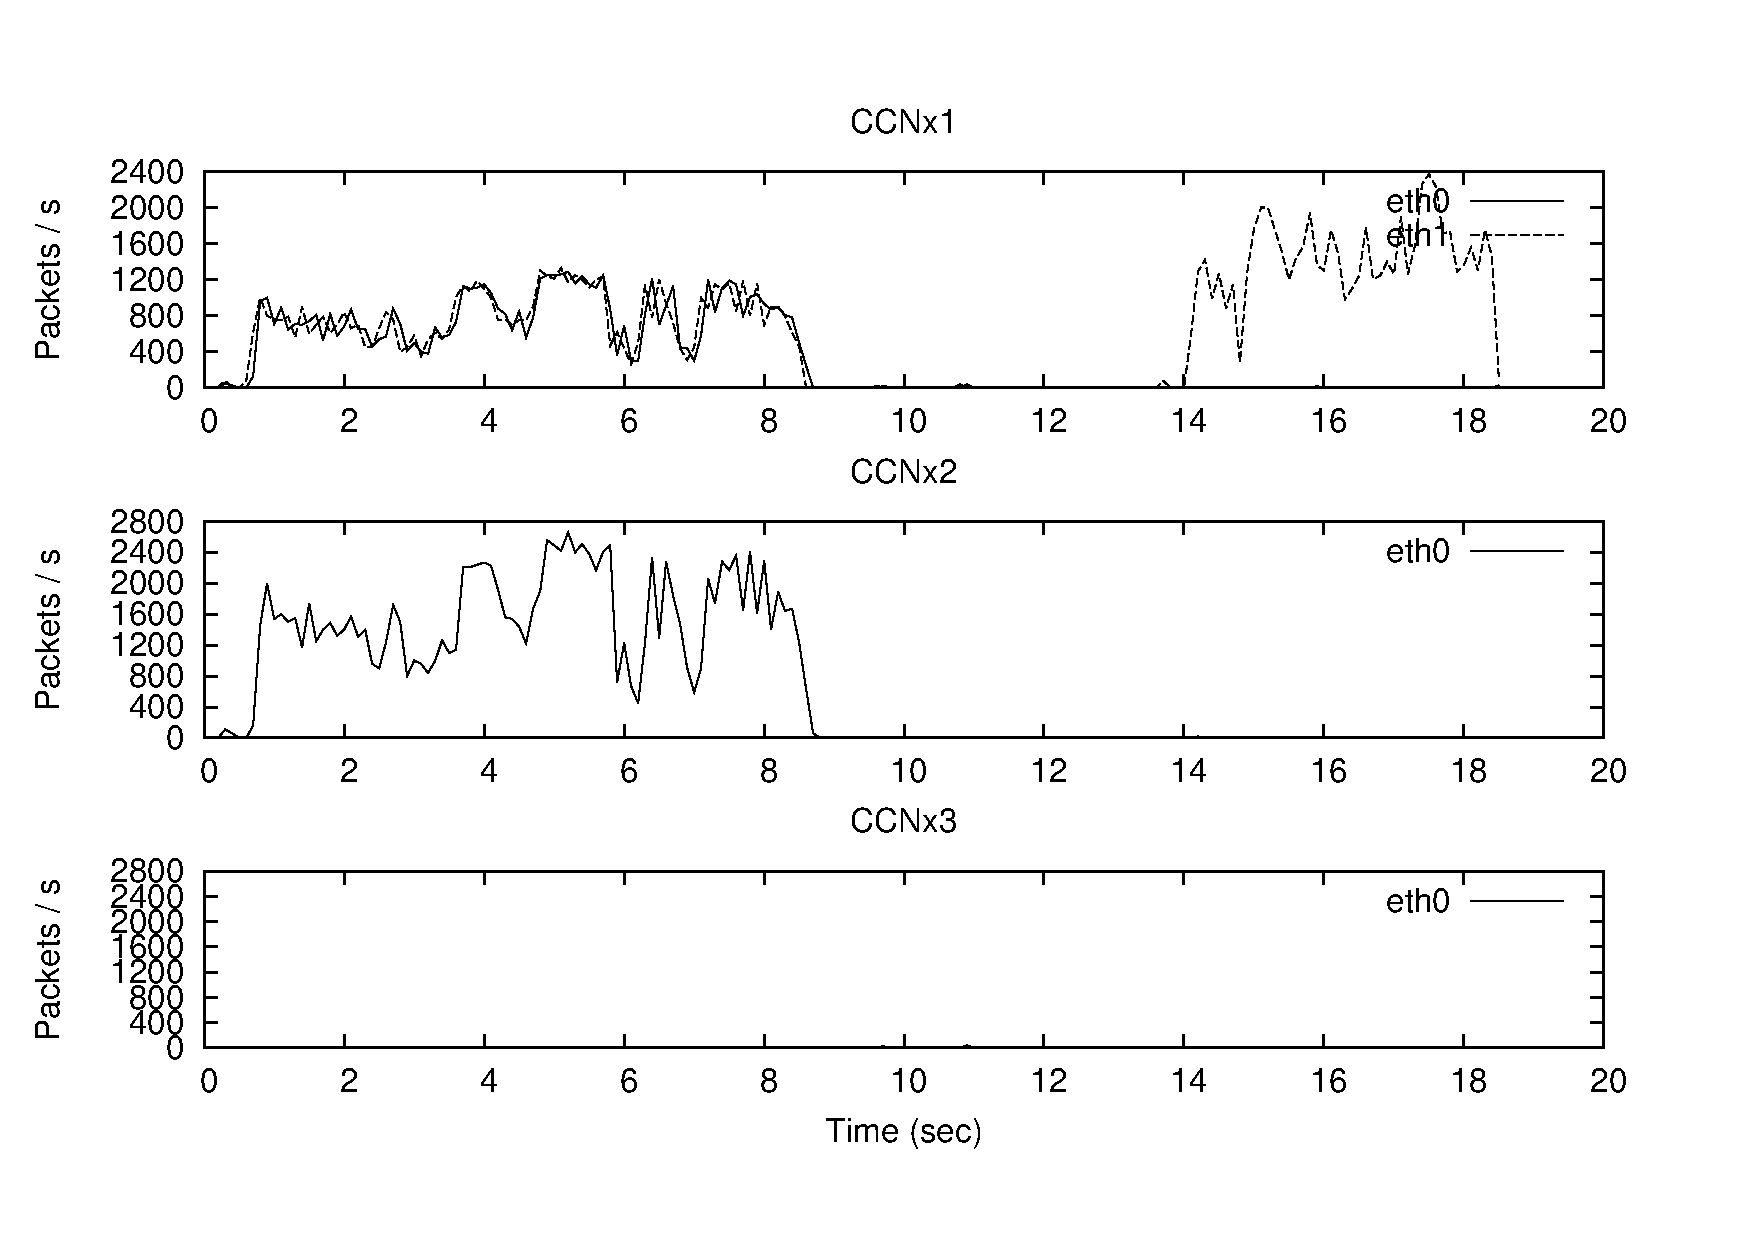
\includegraphics[width=0.75\textwidth] {figures/short-route-net.pdf}
        \label{subfig:short-route-net-app}
    }

    \cprotect\caption{Results for Test 2.3: Network load at 
        all CCNx nodes, during the transfer of a file of size 5\,MB 
        (non-overlapping case), using the `short' path indicated in 
        Figure~\ref{fig:testbed-multiple-paths}.}
    \label{fig:short-route-app}

\end{figure}

\begin{figure}[H]
    \centering

    \subfigure[]{
        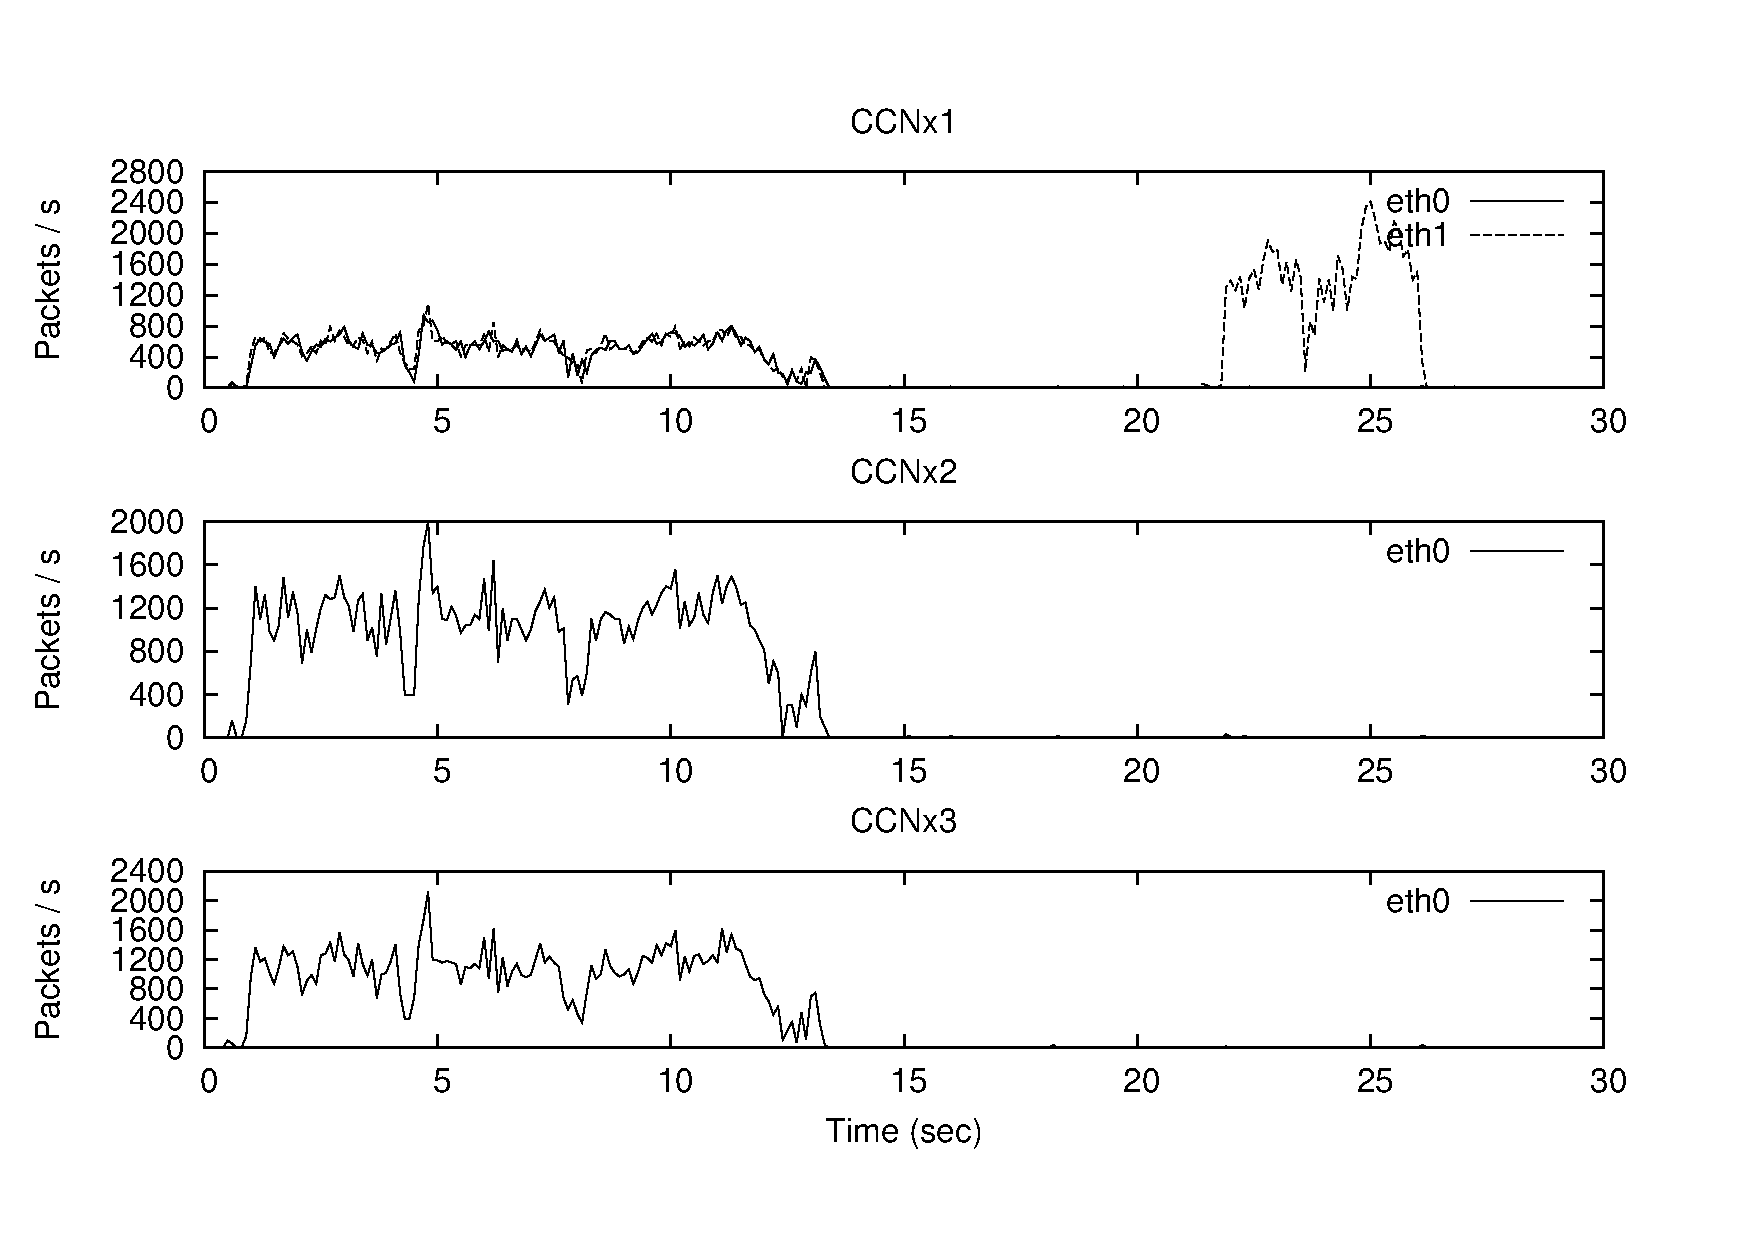
\includegraphics[width=0.75\textwidth] {figures/long-route-net.pdf}
        \label{subfig:long-route-net-app}
    }

    \subfigure[]{
        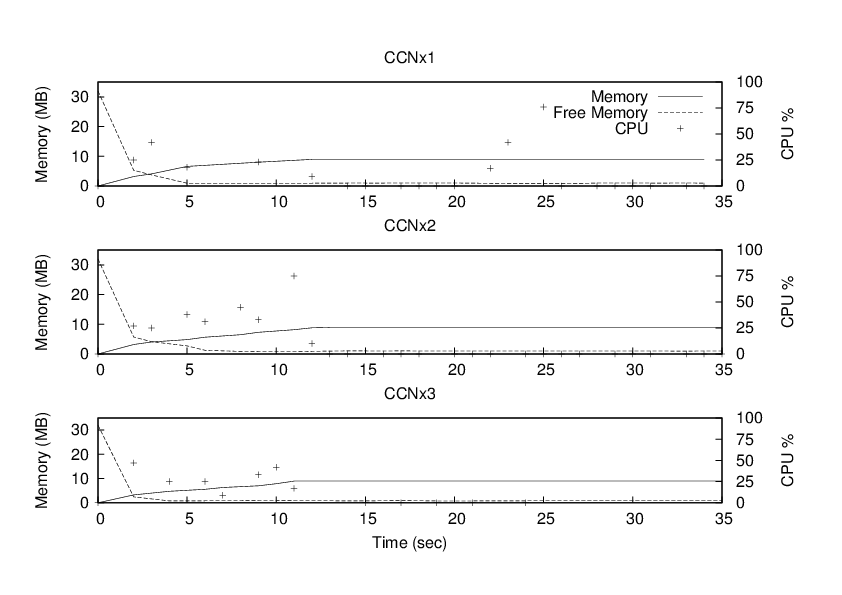
\includegraphics[width=0.75\textwidth] {figures/file_5-long-route-cpu-mem.pdf}
        \label{subfig:long-route-app}
    }

    \cprotect\caption{Results for Test 2.3: Network load (a) and and 
        CPU and memory utilization (b) at 
        all CCNx nodes, during the transfer of a file of size 5\,MB 
        (non-overlapping case), using the `long' path indicated in 
        Figure~\ref{fig:testbed-multiple-paths}. Regarding the 
        memory values, the `memory' line corresponds to the amount of RAM 
        occupied by the \verb+ccnd+ process, while the `free memory' corresponds 
        to the amount of free memory in the system.}
    \label{fig:long-route-app}

\end{figure}

\begin{figure}[H]
    \centering

    \subfigure[]{
        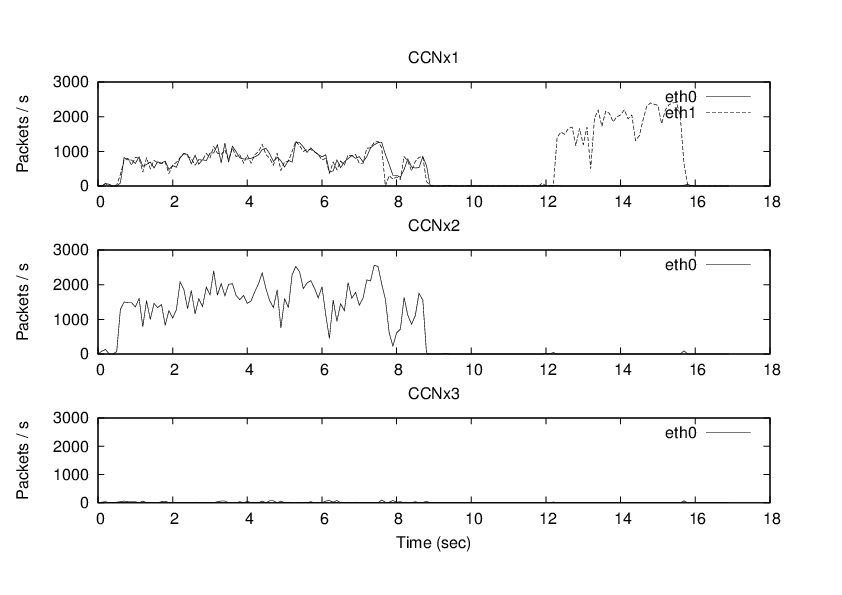
\includegraphics[width=0.75\textwidth] {figures/long-short-route-net.pdf}
        \label{subfig:long-short-route-net-app}
    }

    \subfigure[]{
        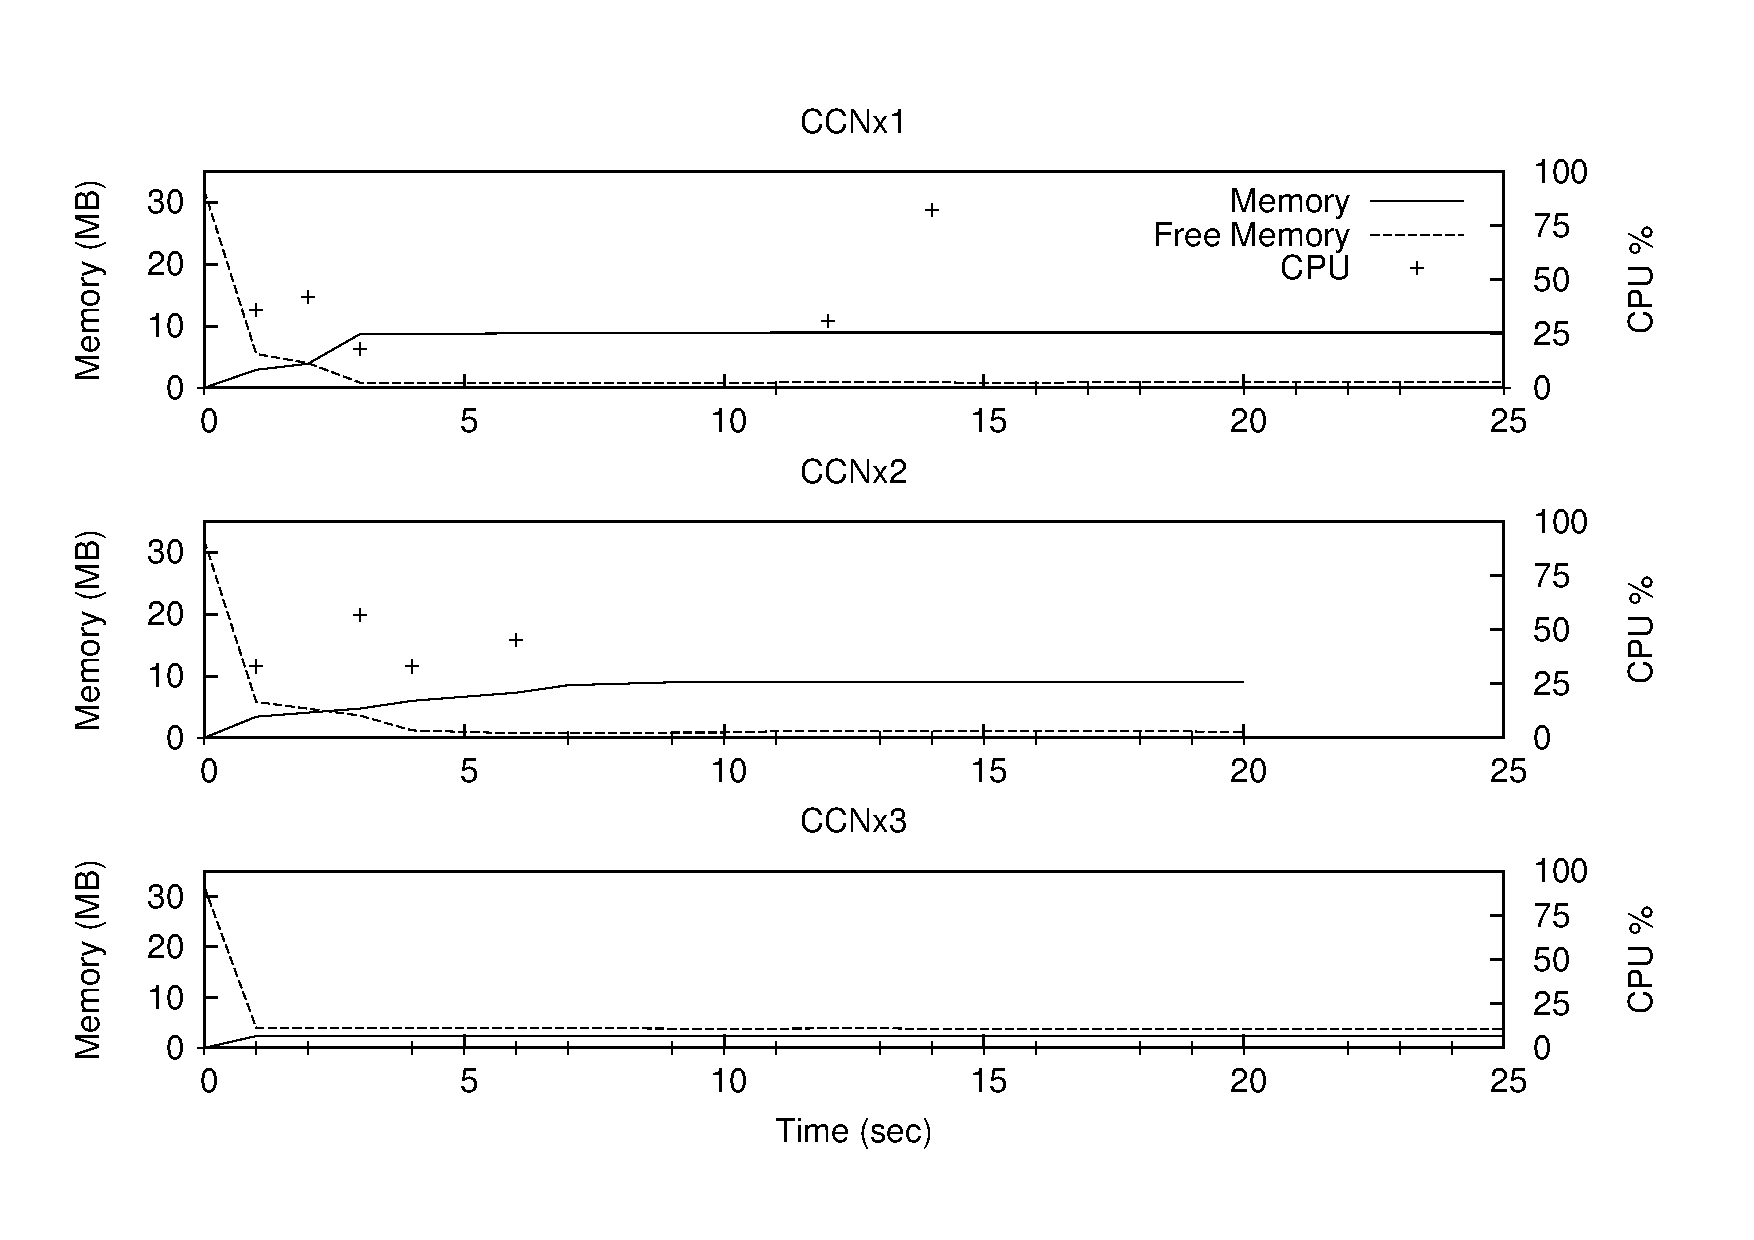
\includegraphics[width=0.75\textwidth] {figures/file_5-long-short-route-cpu-mem.pdf}
        \label{subfig:long-short-route-app}
    }

    \cprotect\caption{Results for Test 2.3: Network load (a) and and 
        CPU and memory utilization (b) at 
        all CCNx nodes, during the transfer of a file of size 5\,MB 
        (non-overlapping case), using both `short' and `long' paths indicated in 
        Figure~\ref{fig:testbed-multiple-paths}. Regarding the 
        memory values, the `memory' line corresponds to the amount of RAM 
        occupied by the \verb+ccnd+ process, while the `free memory' corresponds 
        to the amount of free memory in the system.}
    \label{fig:long-short-route-app}

\end{figure}


%-----------------------------------------------------------
\end{document}
